\documentclass[12pt,]{book}
\usepackage{lmodern}
\usepackage{amssymb,amsmath}
\usepackage{ifxetex,ifluatex}
\usepackage{fixltx2e} % provides \textsubscript
\ifnum 0\ifxetex 1\fi\ifluatex 1\fi=0 % if pdftex
  \usepackage[T1]{fontenc}
  \usepackage[utf8]{inputenc}
\else % if luatex or xelatex
  \ifxetex
    \usepackage{mathspec}
  \else
    \usepackage{fontspec}
  \fi
  \defaultfontfeatures{Ligatures=TeX,Scale=MatchLowercase}
\fi
% use upquote if available, for straight quotes in verbatim environments
\IfFileExists{upquote.sty}{\usepackage{upquote}}{}
% use microtype if available
\IfFileExists{microtype.sty}{%
\usepackage{microtype}
\UseMicrotypeSet[protrusion]{basicmath} % disable protrusion for tt fonts
}{}
\usepackage[margin=1in]{geometry}
\usepackage{hyperref}
\hypersetup{unicode=true,
            pdftitle={Psychophysiological characteristics of verbal rumination},
            pdfborder={0 0 0},
            breaklinks=true}
\urlstyle{same}  % don't use monospace font for urls
\usepackage{natbib}
\bibliographystyle{apalike}
\usepackage{color}
\usepackage{fancyvrb}
\newcommand{\VerbBar}{|}
\newcommand{\VERB}{\Verb[commandchars=\\\{\}]}
\DefineVerbatimEnvironment{Highlighting}{Verbatim}{commandchars=\\\{\}}
% Add ',fontsize=\small' for more characters per line
\usepackage{framed}
\definecolor{shadecolor}{RGB}{248,248,248}
\newenvironment{Shaded}{\begin{snugshade}}{\end{snugshade}}
\newcommand{\KeywordTok}[1]{\textcolor[rgb]{0.13,0.29,0.53}{\textbf{#1}}}
\newcommand{\DataTypeTok}[1]{\textcolor[rgb]{0.13,0.29,0.53}{#1}}
\newcommand{\DecValTok}[1]{\textcolor[rgb]{0.00,0.00,0.81}{#1}}
\newcommand{\BaseNTok}[1]{\textcolor[rgb]{0.00,0.00,0.81}{#1}}
\newcommand{\FloatTok}[1]{\textcolor[rgb]{0.00,0.00,0.81}{#1}}
\newcommand{\ConstantTok}[1]{\textcolor[rgb]{0.00,0.00,0.00}{#1}}
\newcommand{\CharTok}[1]{\textcolor[rgb]{0.31,0.60,0.02}{#1}}
\newcommand{\SpecialCharTok}[1]{\textcolor[rgb]{0.00,0.00,0.00}{#1}}
\newcommand{\StringTok}[1]{\textcolor[rgb]{0.31,0.60,0.02}{#1}}
\newcommand{\VerbatimStringTok}[1]{\textcolor[rgb]{0.31,0.60,0.02}{#1}}
\newcommand{\SpecialStringTok}[1]{\textcolor[rgb]{0.31,0.60,0.02}{#1}}
\newcommand{\ImportTok}[1]{#1}
\newcommand{\CommentTok}[1]{\textcolor[rgb]{0.56,0.35,0.01}{\textit{#1}}}
\newcommand{\DocumentationTok}[1]{\textcolor[rgb]{0.56,0.35,0.01}{\textbf{\textit{#1}}}}
\newcommand{\AnnotationTok}[1]{\textcolor[rgb]{0.56,0.35,0.01}{\textbf{\textit{#1}}}}
\newcommand{\CommentVarTok}[1]{\textcolor[rgb]{0.56,0.35,0.01}{\textbf{\textit{#1}}}}
\newcommand{\OtherTok}[1]{\textcolor[rgb]{0.56,0.35,0.01}{#1}}
\newcommand{\FunctionTok}[1]{\textcolor[rgb]{0.00,0.00,0.00}{#1}}
\newcommand{\VariableTok}[1]{\textcolor[rgb]{0.00,0.00,0.00}{#1}}
\newcommand{\ControlFlowTok}[1]{\textcolor[rgb]{0.13,0.29,0.53}{\textbf{#1}}}
\newcommand{\OperatorTok}[1]{\textcolor[rgb]{0.81,0.36,0.00}{\textbf{#1}}}
\newcommand{\BuiltInTok}[1]{#1}
\newcommand{\ExtensionTok}[1]{#1}
\newcommand{\PreprocessorTok}[1]{\textcolor[rgb]{0.56,0.35,0.01}{\textit{#1}}}
\newcommand{\AttributeTok}[1]{\textcolor[rgb]{0.77,0.63,0.00}{#1}}
\newcommand{\RegionMarkerTok}[1]{#1}
\newcommand{\InformationTok}[1]{\textcolor[rgb]{0.56,0.35,0.01}{\textbf{\textit{#1}}}}
\newcommand{\WarningTok}[1]{\textcolor[rgb]{0.56,0.35,0.01}{\textbf{\textit{#1}}}}
\newcommand{\AlertTok}[1]{\textcolor[rgb]{0.94,0.16,0.16}{#1}}
\newcommand{\ErrorTok}[1]{\textcolor[rgb]{0.64,0.00,0.00}{\textbf{#1}}}
\newcommand{\NormalTok}[1]{#1}
\usepackage{longtable,booktabs}
\usepackage{graphicx,grffile}
\makeatletter
\def\maxwidth{\ifdim\Gin@nat@width>\linewidth\linewidth\else\Gin@nat@width\fi}
\def\maxheight{\ifdim\Gin@nat@height>\textheight\textheight\else\Gin@nat@height\fi}
\makeatother
% Scale images if necessary, so that they will not overflow the page
% margins by default, and it is still possible to overwrite the defaults
% using explicit options in \includegraphics[width, height, ...]{}
\setkeys{Gin}{width=\maxwidth,height=\maxheight,keepaspectratio}
\IfFileExists{parskip.sty}{%
\usepackage{parskip}
}{% else
\setlength{\parindent}{0pt}
\setlength{\parskip}{6pt plus 2pt minus 1pt}
}
\setlength{\emergencystretch}{3em}  % prevent overfull lines
\providecommand{\tightlist}{%
  \setlength{\itemsep}{0pt}\setlength{\parskip}{0pt}}
\setcounter{secnumdepth}{5}
% Redefines (sub)paragraphs to behave more like sections
\ifx\paragraph\undefined\else
\let\oldparagraph\paragraph
\renewcommand{\paragraph}[1]{\oldparagraph{#1}\mbox{}}
\fi
\ifx\subparagraph\undefined\else
\let\oldsubparagraph\subparagraph
\renewcommand{\subparagraph}[1]{\oldsubparagraph{#1}\mbox{}}
\fi

%%% Use protect on footnotes to avoid problems with footnotes in titles
\let\rmarkdownfootnote\footnote%
\def\footnote{\protect\rmarkdownfootnote}

%%% Change title format to be more compact
\usepackage{titling}

% Create subtitle command for use in maketitle
\newcommand{\subtitle}[1]{
  \posttitle{
    \begin{center}\large#1\end{center}
    }
}

\setlength{\droptitle}{-2em}

  \title{Psychophysiological characteristics of verbal rumination}
    \pretitle{\vspace{\droptitle}\centering\huge}
  \posttitle{\par}
    \author{}
    \preauthor{}\postauthor{}
    \date{}
    \predate{}\postdate{}
  
\usepackage{tikz}
\usepackage{lscape}
\usepackage{indentfirst}
\usepackage{float}
\usepackage[flushleft]{threeparttable}
\usepackage[fulladjust]{marginnote}
\usepackage{tcolorbox}
\usepackage{pdfpages}
\usetikzlibrary{intersections}
\tcbuselibrary{listings,breakable}
\usepackage{pifont}
\usepackage{hyperref}
\usepackage[utf8]{inputenc}
\usepackage{graphicx,pdflscape}
\usepackage{geometry}
\usepackage{float}
\usepackage{longtable}
\usepackage{supertabular}
\usepackage{subfig}
\usepackage{scrextend}
\usepackage{tabularx}
\usepackage{lscape}
\usepackage{tabu}
\usepackage{array}
\usepackage[gen]{eurosym}
\usepackage{subfig}
\usepackage{stackrel,amssymb}
\usepackage{textcomp}
\usepackage{setspace}

\usepackage{booktabs,caption,fixltx2e}
\usepackage[none]{hyphenat}

% for the cover page
\usepackage[a4paper]{meta-donnees}
\usepackage{lmodern}

%%%%%%%%%%%%%%%%%%%%%%%%%%%%%%%%%%%%%%%%%%%%%%%%%%%%%%%%%%%%%%%%%%%%%%%%%%%%%%%%%%%%%%%%%%
% below is the by-default configuration of bookdown-demo
% https://github.com/rstudio/bookdown-demo/blob/master/preamble.tex
%%%%%%%%%%%%%%%%%%%%%%%%%%%%%%%%%%%%%%%%%%%%%%%%%%%%%%%%%%%%%%%%%%%%%%%%%%%%%%%%

\usepackage{graphicx}
\usepackage{amsthm}

\makeatletter
\def\thm@space@setup{%
  \thm@preskip=8pt plus 2pt minus 4pt
  \thm@postskip=\thm@preskip
}
\makeatother

%%%%%%%%%%%%%%%%%%%%%%%%%%%%%%%%
% remove default title
% https://stackoverflow.com/questions/45963505/coverpage-and-copyright-notice-before-title-in-r-bookdown
%%%%%%%%%%%%%%%%%%%%%%%%%%

\let\oldmaketitle\maketitle
\AtBeginDocument{\let\maketitle\relax}

\begin{document}
\maketitle

%\pdfbookmark[0]{Title}{title}
%\maketitle

%%%%%%%%%%%%%%%%%%%%%%%%%%%%%%%%%%%%%%%%%%%%%%%%%%%%%%%%
% Title information
%%%%%%%%%%%%%%%%%%%%%%%%%%%%%%%%%%%%%%%%%%

\Specialite{Cognitive Sciences, Psychology, Neurocognition \& \\ Educational Sciences}
\Arrete{May 25 2016}
\Auteur{Ladislas Nalborczyk}
\Directeur{Pr. Elsa Spinelli \& Pr. Ernst Koster}
\CoDirecteur{Dr. Hélène L\oe venbruck \& Dr. Marcela Perrone-Bertolotti}

% Lab(s)
\Laboratoire{Laboratoire de Psychologie et NeuroCognition \& \\ Psychopathology and Affective Neuroscience Laboratory}

% Doctoral school(s)
\EcoleDoctorale{the doctoral school EDISCE (Grenoble) and the Doctoral School of Social and Behavioural Sciences (Ghent)}

% Title
\Titre{Psychophysiological characteristics\\ of verbal rumination}

% Sub-title
\Soustitre{Basic and clinical aspects}

% defense date
\Depot{November XX 2019}

\Jury{

\UGTPresident{XXXX}{...}
%\UGTPresidente{XXXX}{...}

\UGTRapporteur{XXXX}{...}
\UGTRapporteur{XXXX}{...}

\UGTExaminatrice{XXXX}{...}
\UGTExaminatrice{XXXX}{...}

\UGTDirecteur{Elsa Spinelli}{...}
\UGTCoEncandrant{Ernst Koster}{...}
}

%\frontmatter
\MakeUGthesePDG
\cleardoublepage

{
\setcounter{tocdepth}{3}
\tableofcontents
}
\listoftables
\listoffigures
\chapter*{Acknowledgments}\label{acknowledgments}
\addcontentsline{toc}{chapter}{Acknowledgments}

Acknowledgemnents are not yet available.

\chapter*{Abstract}\label{abstract}
\addcontentsline{toc}{chapter}{Abstract}

\ldots{}

\part{Theoretical
framework}\label{part-theoretical-framework}

\chapter{Overt and imagined actions}\label{intro}

Blah blah \citep{koster_rumination_2013}\ldots{}

Wittgenstein's (1953) famous query: ``When I raise my arm, what is left
after subtracting the fact that my arm raised?''. We posit that what is
left is an internal model (a representation) of what should happen if
and when my arm goes up (Jeannerod, 1999)\ldots{}

\section{Motor imagery}\label{motor-imagery}

Considerable experimental evidence has accumulated to suggest that
movement execution and MI share substantial overlap of active brain
regions (for review, see Guillot et al., 2012). Such apparent functional
equivalence supports the hypothesis that MI draws on the similar neural
networks that are used in actual perception and motor control
(Jeannerod, 1994; Grezes and Decety, 2001; Holmes and Collins,
2001)\ldots{}

See introduction of O'Shea (2017) phd thesis introduction\ldots{}

See Stinear's chapter in Guillot's book for intracortical and spinal
mechanisms involved during motor imagery (p.55-57).

\subsection{Simulation theories}\label{simulation-theories}

\ldots{}

For Jeannerod (1995), motor imagery is necessarily first-perspective.
Third perspective imagery is imagery, but not MOTOR imagery\ldots{}
Motor representations are conceived here as `internal models' of the
goal of an action.

\subsection{Emulation theories}\label{emulation-theories}

\ldots{}

\subsection{Action representation and internal
models}\label{action-representation-and-internal-models}

Voir Jeannerod (2004), Wolpert el al. (1995), Wolpert \& Gharamani
(2000)\ldots{}

\section{Inner speech}\label{inner-speech}

\ldots{}

The inner voice as the sensory consequence (prediction, see Loevenbruck
et al., 2018) of imagined speech. Analogy with raising the arm: what we
perceive when we imagine raising our arm are the sensory consequences
(e.g., visual) of what would happen if we actually raised our arm, these
are then kind of predictions. The same thing happens during inner speech
production: the inner voice is the predicted auditory consequence of
actual speech, except that it's predicted. The two actions might seem
very different, partly because of differences in the degree of
automaticity. Imagining raising our arm might need a
voluntary/deliberate/conscious (choose a word) intention (i.e., I want
to raise my arm \textgreater{} I raise my arm) while speech imagery
(i.e., inner speech) seems more automatic: we do not expression
consciously the intention to speak, we just speak\ldots{}

\subsection{MVTV Cohen (1986)}\label{mvtv-cohen-1986}

\ldots{}

\subsection{Predictive models}\label{predictive-models}

Learning how to internalise speech might be similar to learning how to
internalise playing an instrument\ldots{} Let's consider the analogy
between speaking and playing an instrument (e.g., the piano). Playing
piano results from the learning of an infinitely complex coordination of
fine motor sequences, that in turn produce sensory (kinestheatic,
auditory, visual, etc) feedback to the producer of the action (the
agent). It seems that (from a certain level of analysis), the act of
speech can be paralleled with the act of playing an instrument in that
its consists in the coordination of infinitely complex movements that
result in some modifications in the environment that in turn generate
sensory feedbacks for the agent. Thus, pursuing the analogy, we argue
that imagining playing pian and imagining speaking (i.e., producing
inner speech) might rest on similar mechanisms\ldots{} see O'Shea \&
Moran (2018) on expert pianists\ldots{}

\chapter{Rumination as simulated
speech}\label{rumination-as-simulated-speech}

As suggested by \citet{Christoff2016}, rumination and other forms of
spontaneous thoughts can be considered in a common conceptual space (see
Figure 1). This space is built upon two dimensions: \emph{deliberate
constraints} and \emph{automatic constraints}. These dimensions
represent two general mechanisms that allow to constrain the contents of
these related mental states and the transitions between them. The first
contrain correspond to a deliberate processus and is implemented through
\textbf{cognitive control} \citep{Miller2000}. The second constrain is
referring to more automatic constrains like sensory afferences. In this
framework, rumination is characterized by the highest level of automatic
constraints and spread all along the \emph{deliberate constraints}
dimension.

\begin{figure}

{\centering 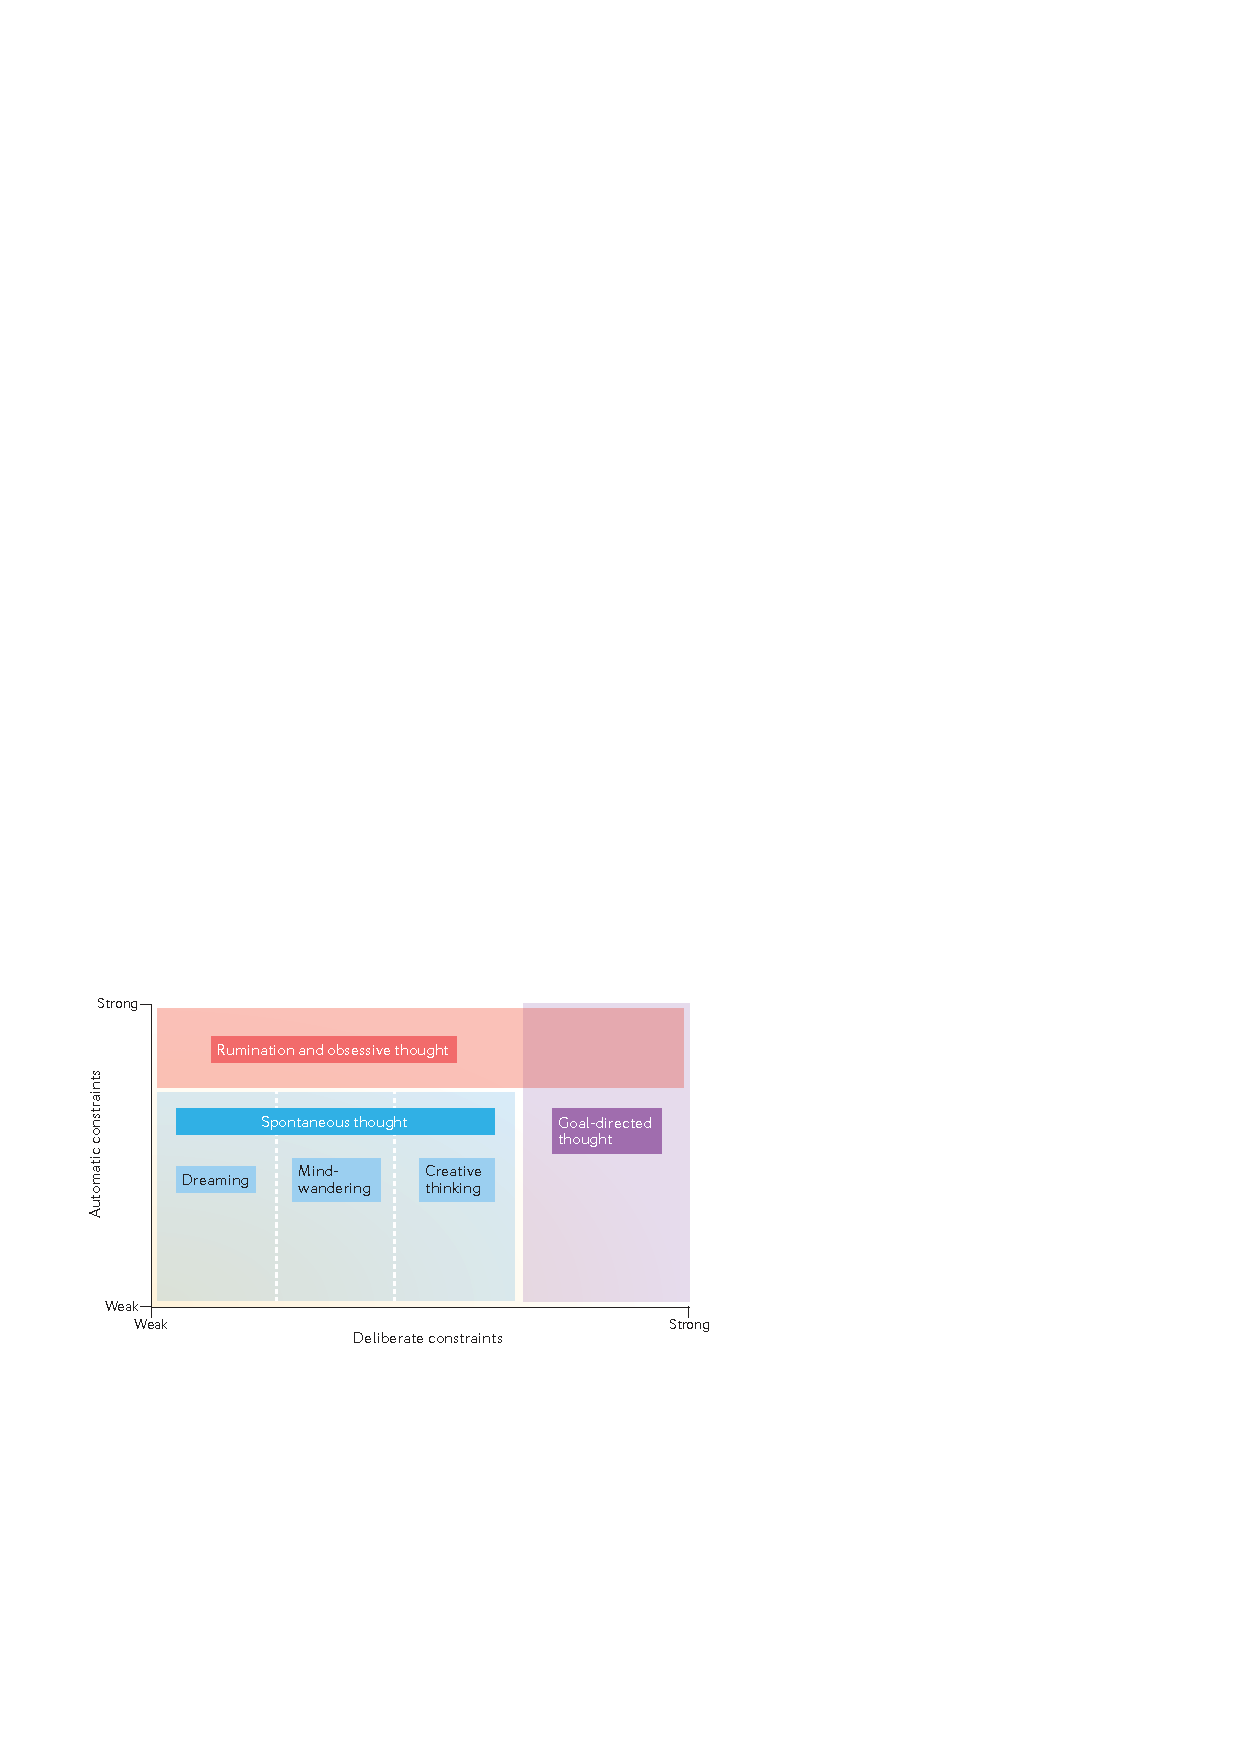
\includegraphics{assets/conceptual_space} 

}

\caption{Conceptual space of different types of thought (Christoff et al., 2016)}\label{fig:unnamed-chunk-1}
\end{figure}

\ldots{}

\chapter{Electromyographic correlates of speech
production}\label{electromyographic-correlates-of-speech-production}

\ldots{}

\section{Speech production
mechanisms}\label{speech-production-mechanisms}

\ldots{}

\section{Speech production muscles}\label{speech-production-muscles}

\ldots{}

\section{Muscular physiology}\label{muscular-physiology}

\ldots{}

\section{EMG signal}\label{emg-signal}

\subsection{EMG signal measures}\label{emg-signal-measures}

Muscular activity can be studied at different levels. At the cellular
level, using electrophysiological measures like micro-electrods
implanted in the cell, that allow direct measures of \textbf{action
potential}. At the segmental level, biomechanis study muscular activity
using surface sensors, positionned on the skin\ldots{}intermediate
levels\ldots{}

\subsection{Motor Unit Action
Potential}\label{motor-unit-action-potential}

\textbf{Motor unit action potential} (MUAP) is the electric field
resulting from the sum f the electric fiels emitted y each fiber of the
motor unit. This train of action potentials will generate a \emph{train}
of MUAP, call \textbf{motor unit action potential trains} (MUAPT). The
electric potential generated by this field is highly dependant of
parameters such as the number of fibers, their length, speed of
conduction and position of the neuromuscular junction.

\begin{figure}

{\centering 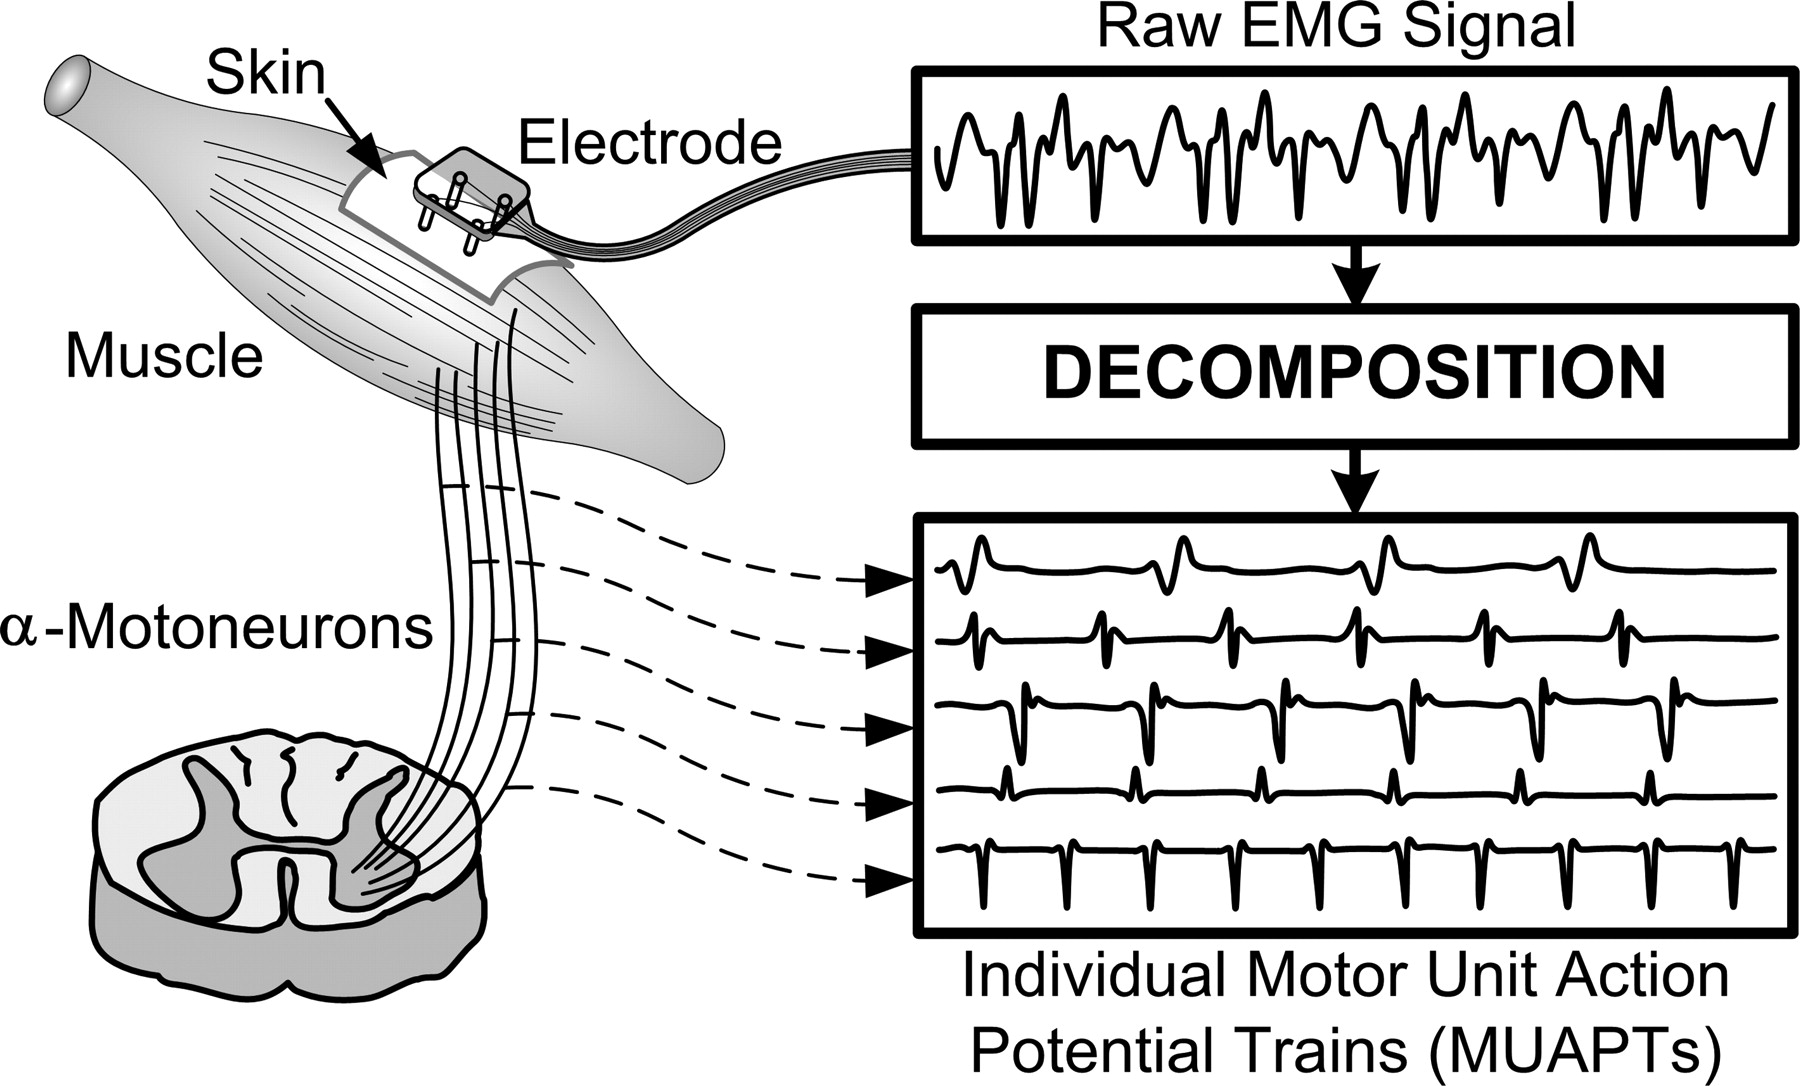
\includegraphics{assets/muap} 

}

\caption{Motor unit action potential schema.}\label{fig:unnamed-chunk-1}
\end{figure}

\ldots{}

EMG signal then result in a mixture of recruited motor units.

\subsection{Surface EMG}\label{surface-emg}

\ldots{}\emph{crosstalk} phenomenon \citep{DeLuca1997}. In reason of the
important\ldots{} of facial muscles, the EMG activity of one recorded
muscle generally does not represent the activity of a single muscle but
rather a mixture of\ldots{}\citet{Rapin2011}\ldots{}

\subsection{Basic signal processing}\label{basic-signal-processing}

\ldots{}the EMG signal is a stochastic signal\ldots{} In order to
illustrate what EMG signal looks like, we simulated EMG signal based on
a standard algorithm \citep[pp.70-71]{Hermens1999}, implemented in R by
\citet{Borg2014}.

\begin{Shaded}
\begin{Highlighting}[]
\OperatorTok{>}\StringTok{ }\KeywordTok{source}\NormalTok{(}\StringTok{"code/EMGfuns.R"}\NormalTok{)}
\OperatorTok{>}\StringTok{ }\NormalTok{emg <-}\StringTok{ }\KeywordTok{EMG_sim}\NormalTok{(}\DataTypeTok{n =} \DecValTok{2048}\NormalTok{, }\DataTypeTok{sampFreq =} \DecValTok{1000}\NormalTok{, }\DataTypeTok{lF =} \DecValTok{10}\NormalTok{, }\DataTypeTok{hF =} \DecValTok{100}\NormalTok{)}\OperatorTok{$}\NormalTok{sim}
\OperatorTok{>}\StringTok{ }\KeywordTok{ts.plot}\NormalTok{(emg, }\DataTypeTok{xlab =} \StringTok{"Time (ms)"}\NormalTok{, }\DataTypeTok{ylab =} \StringTok{"simEMG"}\NormalTok{, }\DataTypeTok{col =} \StringTok{"steelblue"}\NormalTok{)}
\end{Highlighting}
\end{Shaded}

\begin{figure}[h!]

{\centering 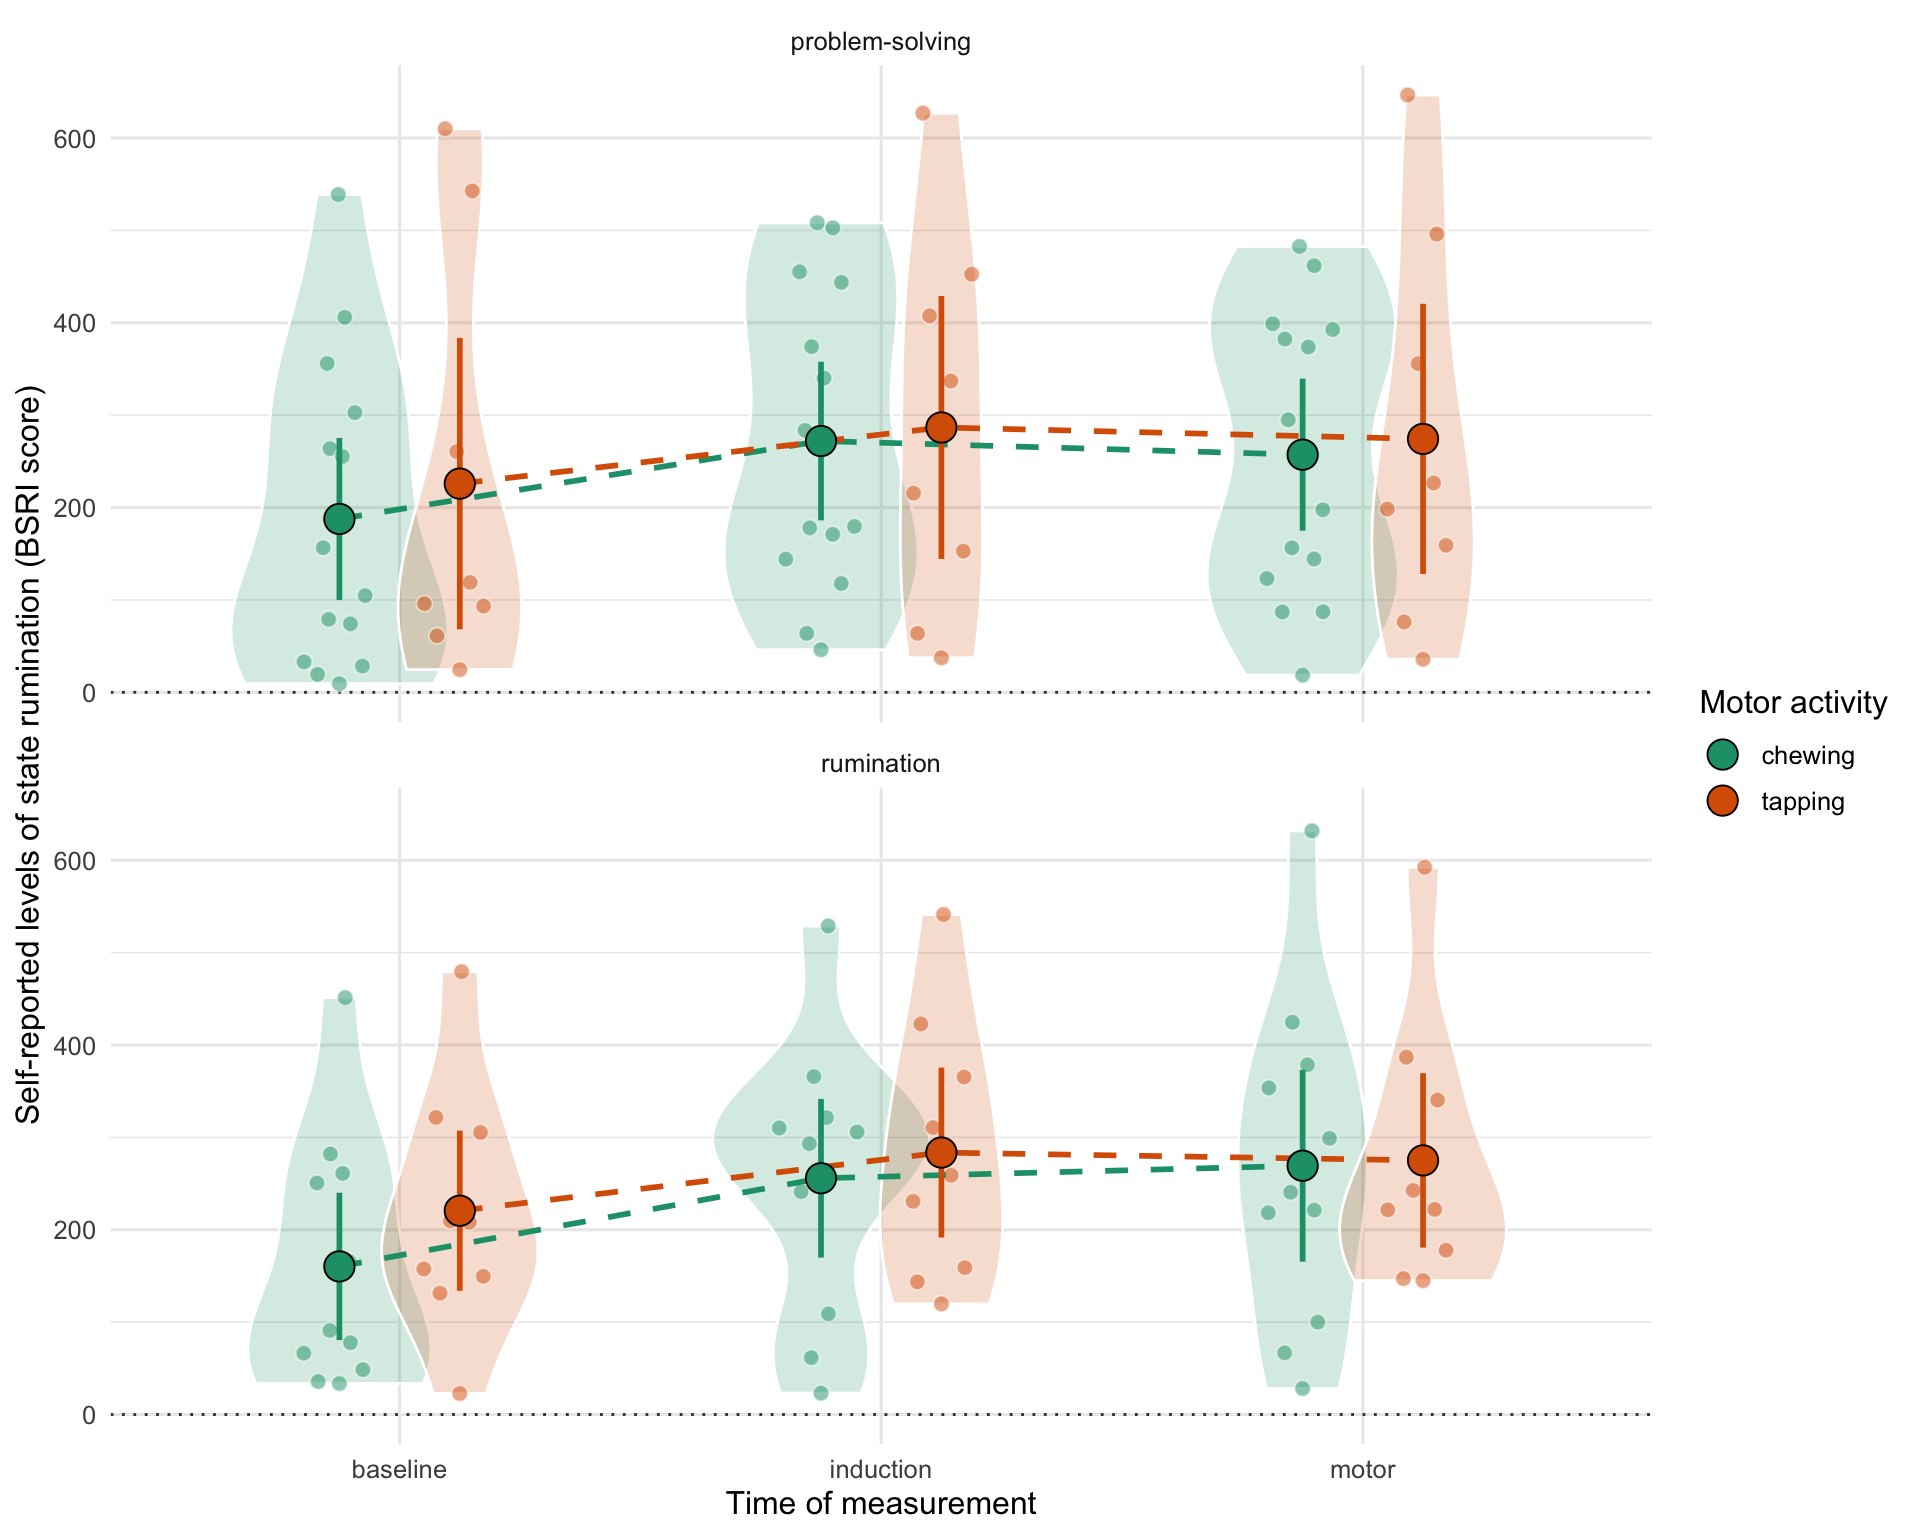
\includegraphics{02-chap2_files/figure-latex/unnamed-chunk-2-1} 

}

\caption{Simulated EMG signal.}\label{fig:unnamed-chunk-2}
\end{figure}

\ldots{}we rectify the EMG signal by taking its absolute value and
substracting the mean in order to correct for any offset (bias) present
in the raw data. It is interesting to note that the effects of
rectification on the EMG signal is similar to the rectification of AM
radio waves whose purpose is to enhance the low frequency components,
wich encode the voice signals. Concerning EMG, the ``voice'' of the
signal corresponds to the encoded force \citep{Borg2007}.

\begin{Shaded}
\begin{Highlighting}[]
\OperatorTok{>}\StringTok{ }\NormalTok{emg <-}\StringTok{ }\KeywordTok{abs}\NormalTok{(emg }\OperatorTok{-}\StringTok{ }\KeywordTok{mean}\NormalTok{(emg) )}
\OperatorTok{>}\StringTok{ }\KeywordTok{ts.plot}\NormalTok{(emg, }\DataTypeTok{xlab =} \StringTok{"Time (ms)"}\NormalTok{, }\DataTypeTok{ylab =} \StringTok{"simEMG"}\NormalTok{, }\DataTypeTok{col =} \StringTok{"steelblue"}\NormalTok{)}
\end{Highlighting}
\end{Shaded}

\begin{figure}[h!]

{\centering 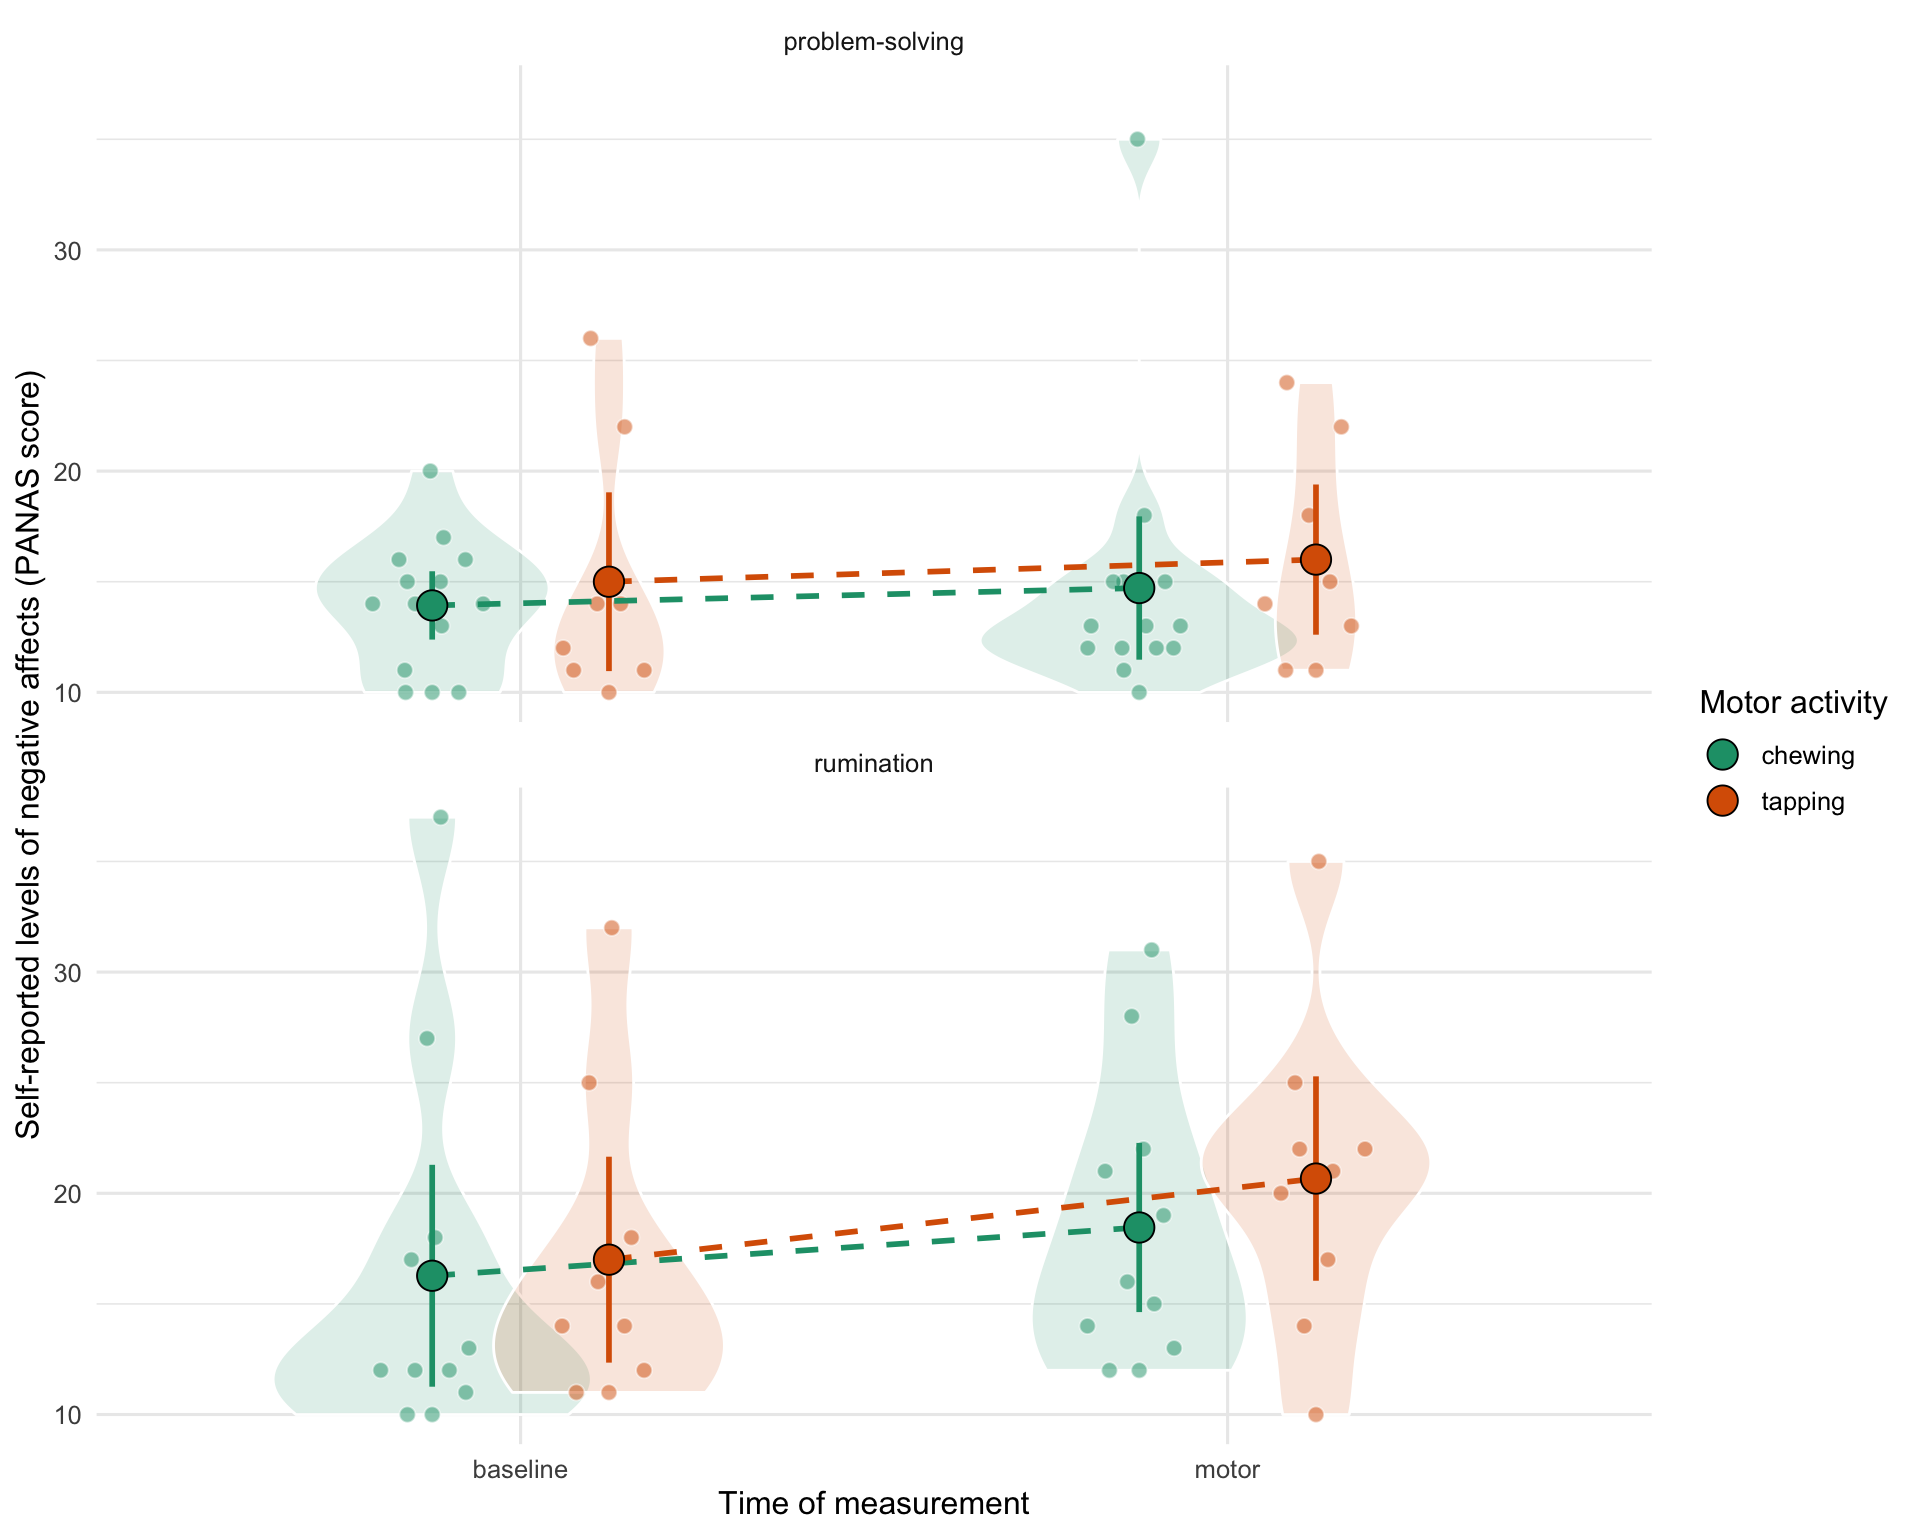
\includegraphics{02-chap2_files/figure-latex/unnamed-chunk-3-1} 

}

\caption{Rectified EMG signal.}\label{fig:unnamed-chunk-3}
\end{figure}

\ldots{}

There are two main measures thant can be used to represent the magnitude
of muscle activity. These two measures can be directly computed from the
filtered EMG signal. The first one is the \textbf{average rectified
value} (ARV):

\[ARV = \frac{1}{T} \sum_{t=1}^{T} | EMG(t_{i}) |\]

which is computed over a specific interval \((0,T)\) and where
\(|EMG(_{i})|\) is the absolute value of a datum of EMG in the data
window. The unit of measurement is \(mV\) or \(\mu V\), and the ARV
calculation is generally similar to the numerical formula for
integration \citep{Kamen2010}.

The second one is the \textbf{root-mean-square} (RMS) amplitude:

\[RMS = \sqrt \frac{1}{T} \sum_{t=1}^{T} | EMG^{2}(t_{i}) |\]

where \(|EMG^{2}(_{i})|\) is the squared value of each EMG datum and has
both physical and physiological meanings\ldots{}

\part{Experimental part}\label{part-experimental-part}

Blah blah blah\ldots{} explain why two parts\ldots{}

\chapter{Orofacial electromyographic correlates of induced verbal
rumination}\label{orofacial-electromyographic-correlates-of-induced-verbal-rumination}

Summary of the research\ldots{}\footnote{This experimental chapter is a
  published paper reformatted for the need of this thesis. Source:
  Nalborczyk, L., Perrone-Bertolotti, M., Baeyens, C., Grandchamp, R.,
  Polosan, M., Spinelli, E., \ldots{} L\oe venbruck, H. (2017).
  Orofacial Electromyographic Correlates of Induced Verbal Rumination.
  \emph{Biological Psychology, 127}, 53-63.
  \url{http://dx.doi.org/10.1016/j.biopsycho.2017.04.013}.}

\section{Introduction}\label{introduction}

As humans, we spend a considerable amount of time reflecting upon
ourselves, thinking about our own feelings, thoughts and behaviors.
Self-reflection enables us to create and clarify the meaning of past and
present experiences (Boyd \& Fales, 1983; Nolen-Hoeksema, Wisco, \&
Lyubomirsky, 2008). However, this process can lead to unconstructive
consequences when self-referent thoughts become repetitive, abstract,
evaluative, and self-critical (Watkins, 2008).

Indeed, rumination is most often defined as a repetitive and recursive
mode of responding to negative affect (Rippere, 1977) or life situations
(Robinson \& Alloy, 2003). Although rumination is a common process that
can be observed in the general population (Watkins, 2008), it has been
most extensively studied in depression and anxiety. Depressive
rumination has been thoroughly studied by Susan Nolen- Hoeksema, who
developed the Response Style Theory (RST; Nolen-Hoeksema, 1991).
According to the RST, depressive rumination is characterized by an
evaluative style of processing that involves recurrent thinking about
the causes, meanings, and implications of depressive symptoms. Even
though rumination can involve several modalities (i.e., visual,
sensory), it is a predominantly verbal process (Goldwin \& Behar, 2012;
McLaughlin, Borkovec, \& Sibrava, 2007). In this study, we focus on
verbal rumination, which can be conceived of as a particularly
significant form of inner speech.

Inner speech or covert speech can be defined as silent verbal production
in one's mind or the activity of silently talking to oneself (Zivin,
1979). The nature of inner speech is still a matter of theoretical
debate (see Perrone-Bertolotti, Rapin, Lachaux, Baciu, \& L \& venbruck,
2014 for a review). Two opposing views have been proposed in the
literature: the Abstraction view and the Motor Simulation view. The
Abstraction view describes inner speech as unconcerned with articula-
tory or auditory simulations and as operating on an amodal level. It has
been described as ``condensed, abbreviated, disconnected, fragmented,
and incomprehensible to others'' (Vygotsky, 1987). It has been argued
that important words or grammatical affixes may be dropped in inner
speech (Vygotsky, 1987) or even that the phonological form or
representation of inner words may be incomplete (Sokolov, 1972; Dell \&
Repka, 1992). MacKay (1992) stated that inner speech is nonarticulatory
and nonauditory and that ``Even the lowest level units for inner speech
are highly abstract'' (p.122).

In contrast with this Abstraction view, the physicalist or embodied view
considers inner speech production as mental simulation of overt speech
production. As such, it can be viewed as similar to overt speech
production, except that the motor execution process is blocked and no
sound is produced (Grèzes \& Decety, 2001; Postma \& Noordanus, 1996).
Under this Motor Simulation view, a continuum exists between overt and
covert speech, in line with the continuum drawn by Decety and Jeannerod
(1996) between imagined and actual actions. This hypoth- esis has led
certain authors to claim that inner speech by essence should share
features with speech motor actions (Feinberg, 1978; Jones \& Fernyhough,
2007). The Motor Simulation view is supported by several findings.
Firstly, covert and overt speech have comparable physiological
correlates: for instance, measurements of speaking rate (Landauer, 1962;
Netsell, Ashley, \& Bakker, 2010) and respiratory rate (Conrad \&
Schönle, 1979) are similar in both. A prediction of the Motor Simulation
view is that the speech motor system should be recruited during inner
speech. Subtle muscle activity has been detected in the speech
musculature using electromyography (EMG) during verbal mental imagery,
silent reading, silent recitation (Jacobson, 1931; Sokolov, 1972;
Livesay, Liebke, Samaras, \& Stanley, 1996; McGuigan \& Dollins, 1989),
and during auditory verbal hallucination in patients with schizophrenia
(Rapin, Dohen, Polosan, Perrier, \& L \& venbruck, 2013). Secondly, it
has been shown that covert speech production involves a similar cerebral
network as that of overt speech production. Covert and overt speech both
recruit essential language areas in the left hemisphere (for a review,
see Perrone- Bertolotti et al., 2014). However, there are differences.
Consistent with the Motor Simulation view and the notion of a continuum
between covert and overt speech, overt speech is associated with more
activity in motor and premotor areas than inner speech (e.g., Palmer et
al., 2001). This can be related to the absence of articulatory movements
during inner verbal production. In a reciprocal way, inner speech
involves cerebral areas that are not activated during overt speech
(Basho, Palmer, Rubio, Wulfeck, \& Müller, 2007). Some of these
activations (cingulate gyrus and superior rostral frontal cortex) can be
attributed to the inhibition of overt responses.

These findings suggest that the processes involved in overt speech
include those required for inner speech (except for inhibition). Several
studies in patients with aphasia support this view: overt speech loss
can either be associated with an impairment in inner speech (e.g.,
Levine, Calvanio, \& Popovics, 1982; Martin \& Caramazza, 1982) or with
intact inner speech: only the later phases of speech production
(execution) being affected by the lesion (Baddeley \& Wilson, 1985;
Marshall et al., 1985; Vallar \& Cappa, 1987). Geva, Bennett, Warburton,
and Patterson (2011) have reported a dissociation that goes against this
view, however. In three patients with chronic post-stroke aphasia (out
of 27 patients), poorer homophone and rhyme judgement performance was in
fact observed in covert mode compared with overt mode. A limitation of
this study, though, was that the task was to detect rhymes in written
words, which could have been too difficult for the patients. To over-
come this limitation, Langland-Hassan, Faries, Richardson, and Dietz
(2015) have tested aphasia patients with a similar task, using images
rather than written words. They also found that most patients performed
better in the overt than in the covert mode. They inferred from these
results that inner speech might be more demanding in terms of cognitive
and linguistic load, and that inner speech may be a distinct ability,
with its own neural substrates. We suggest an alternative interpretation
to this dissociation. According to our view, rhyme and homophone
judgements rely on auditory representations of the stimuli (see e.g.,
Paulesu, Frith, \& Frackowiak, 1993). Overt speech provides a strong
acoustic output that is fed back to the auditory cortex and can create
an auditory trace, which can be used to monitor speech. In the covert
mode, the auditory output is only mentally simulated, and its saliency
in the auditory system is lesser than in the overt mode. This is in
accordance with the finding that inner speech is associated with reduced
sensory cortex activation compared with overt speech (Shuster \&
Lemieux, 2005). In patients with aphasia, the weakened saliency of
covert auditory signals may be accentuated for two reasons: first,
because of impairment in the motor-to-auditory transformation that
produces the auditory simulation, and second, because of asso- ciated
auditory deficits. Therefore, according to our view, the reduced
performance observed in rhyme and homophone judgement tasks in the
covert compared with the overt mode in brain-injured patients, simply
indicates a lower saliency of the auditory sensations evoked during
inner speech compared with the actual auditory sensations fed back
during overt speech production. In summary, these findings suggest that
overt and covert speech share common subjective, physiological and
neural correlates, supporting the claim that inner speech is a motor
simulation of overt speech.

However, the Motor Simulation view has been challenged by several
experimental results. Examining the properties of errors during the
production of tongue twisters, Oppenheim and Dell (2010) showed that
speech errors display a lexical bias in both overt and inner speech.
According to these researchers, errors also display a phonemic similar-
ity effect (or articulatory bias), a tendency to exchange phonemes with
common articulatory features, but this second effect is only observed
with overt speech or with inner speech accompanied with mouthing. This
has led Oppenheim and Dell (2010) to claim that inner speech is fully
specified at the lexical level, but that it is impoverished at lower
featural (articulatory) levels. This claim, related to the Abstraction
view, is still debated however, as a phonemic similarity effect has been
found by Corley, Brocklehurst and Moat (2011). Their findings suggest
that inner speech is in fact specified at the articulatory level, even
when there is no intention to articulate words overtly. Other findings
however, may still challenge the Motor Simulation view. Netsell et al.
(2010) have examined covert and overt speech in persons who stutter
(PWS) and typical speakers. They have found that PWS were faster in
covert than in overt speech while typical speakers presented similar
overt and covert speech rates. This can be interpreted in favour of the
Abstraction view, in which inner representations are not fully specified
at the articulatory level, which would explain why they are not
disrupted in PWS speech. Altogether, these results suggest that full
articulatory specification may not always be necessary for inner speech
to be produced.

The aim of this study is to examine the physiological correlates of
verbal rumination in an attempt to provide new data in the debate
between motor simulation and abstraction. A prediction of the Motor
Simulation view is that verbal rumination, as a kind of inner speech,
should be accompanied with activity in speech-related facial muscles, as
well as in negative emotion or anxiety-related facial muscles, but
should not involve non-facial muscles (such as arm muscles).
Alternatively, the Abstraction view predicts that verbal rumination
should be associated with an increase in emotion-related facial
activity, without activity in speech-related muscles and non-facial
muscles.

There is strong interest in the examination of physiological correlates
of rumination as traditional assessment of rumination essentially
consists of self-reported measures. The measurement of rumination as
conceptualized by Nolen-Hoeksema (1991) was operationalized by the
development of the Ruminative Response Scale (RRS), which is a subscale
of the response style questionnaire (Nolen-Hoeksema \& Morrow, 1991).
The RRS consists of 22 items that describe responses to dysphoric mood
that are self-focused, symptom-focused, and focused on the causes and
consequences of one's mood. Based on this scale, Treynor, Gonzalez and
Nolen-Hoeksema (2003) have offered a detailed description of rumina-
tion styles and more recently, Watkins (2004, 2008) has further
characterized different modes of rumination. The validity of these
descriptions is nevertheless based on the hypothesis that individuals
have direct and reliable access to their internal states. However, self-
reports increase reconstruction biases (e.g., Brewer, 1986; Conway,
1990) and it is well known that participants have a very low level of
awareness of the cognitive processes that underlie and modulate complex
behaviors (Nisbett \& Wilson, 1977).

In order to overcome these difficulties, some authors have at- tempted
to quantify state rumination and trait rumination more objectively, by
recording physiological or neuroanatomical correlates of rumination (for
a review, see Siegle \& Thayer, 2003). Peripheral physiological
manifestations (e.g., pupil dilation, blood pressure, cardiac rhythm,
cardiac variability) have been examined during induced or chronic
rumination. Vickers and Vogeltanz-Holm (2003) have observed an increase
in systolic blood pressure after rumination induction, suggesting the
involvement of the autonomic nervous system in rumination. Moreover,
galvanic skin response has shown to be increased after a rumination
induction, in highly anxious women (Sigmon, Dorhofer, Rohan, \& Boulard,
2000). According to Siegle and Thayer (2003), disrupted autonomic
activity could provide a reliable physiological correlate of rumination.
In this line, Key, Campbell, Bacon, and Gerin (2008) have observed a
diminution of the high- frequency component of heart rate variability
(HF-HRV) after rumina- tion induction in people with a low tendency to
ruminate (see also Woody, McGeary, \& Gibb, 2014). A consistent link
between persevera- tive cognition and decreased HRV was also found in a
meta-analysis conducted by Ottaviani et al. (2015). Based on these
positive results and on suggestions that labial EMG activity may
accompany inner speech and therefore rumination, our aim was to examine
facial EMG as a potential correlate of rumination and HRV as an index to
examine concurrent validity.

In addition to labial muscular activity, we also recorded forehead
muscular activity (i.e., frontalis muscle) because of its implication in
prototypical expression of sadness (e.g., Ekman, 2003; Kohler et al.,
2004), reactions to unpleasant stimuli (Jäncke, Vogt, Musial, Lutz, \&
Kalveram, 1996), and anxiety or negative emotional state (Conrad \&
Roth, 2007)\footnote{The corrugator supercilii was another potential
  site, as it is sensitive to negative emotions. However, it has been
  claimed to be mostly activated for strong emotions such as
  fear/terror, anger/rage and sadness/grief (Ekman \& Friesen, 1978;
  Sumitsuji, Matsumoto, Tanaka, Kashiwagi, \& Kaneko, 1967). The
  rumination induction used in this study was designed to have
  participants self-reflect and brood over their failure at the IQ-
  test. It was not meant to induce such strong emotions. Several studies
  have reported increased activity in the frontalis muscle at rest in
  anxious or generalized anxiety disorder patients (for a review see
  Conrad \& Roth, 2007). We expected the type of emotional state induced
  by rumination to be closer to anxiety or worry than to strong emotions
  like fear, anger or grief. It was therefore more appropriate to record
  non-speech facial activity in the frontalis rather than in the
  corrugator.}. Our hypothesis was that frontalis activity could be an
accurate electromyographic correlate of induced rumination, as a
negatively valenced mental process.

In this study, we were also interested in the effects of relaxation on
induced rumination. Using a relaxation procedure targeted on muscles
involved in speech production is a further way to test the reciprocity
of the link between inner speech (verbal rumination) and orofacial
muscle activity. If verbal rumination is a kind of action, then its
production should be modulated in return by the effects of relaxation on
speech effectors. This idea is supported by the results of (among
others) Cefidekhanie, Savariaux, Sato and Schwartz (2014), who have
observed substantial perturbations of inner speech production while
participants had to realize forced movements of the articulators.

In summary, the current study aimed at evaluating the Motor Simulation
view and the Abstraction view by using objective and subjective measures
of verbal rumination. To test the involvement of the orofacial motor
system in verbal rumination, we used two basic approaches. In the first
approach, we induced verbal rumination and examined concurrent changes
in facial muscle activity (Experiment 1). In the second approach, we
examined whether orofacial relaxation would reduce verbal rumination
levels (Experiment 2). More specifi- cally, in Experiment 1, we aimed to
provide an objective assessment of verbal rumination using quantitative
physiological measures. Thus, we used EMG recordings of muscle activity
during rumination, focusing on the comparison of speech-related (i.e.,
two lip muscles − orbicularis oris superior and orbicularis oris
inferior) and speech-unrelated (i.e., forehead −frontalis- and forearm −
flexor carpi radialis) muscles. Under the Motor Simulation view, an
increase in lip and forehead EMG activity should be observed after
rumination induction, with no change in forearm EMG activity, associated
with an increase in self-reported rumination. Alternatively, under the
Abstraction view, an increase in forehead activity should be observed,
associated with an increase in self-reported rumination, and no changes
in either lip or forearm activity should be noted.

In Experiment 2, in order to assess the reciprocity of the rumination
and orofacial motor activity relationship, we evaluated the effects of
orofacial relaxation on rumination. More specifically, we compared three
kinds of relaxation: i) Orofacial Relaxation (i.e., lip muscles), ii)
Arm Relaxation (i.e., to differentiate effects specific to
speech-related muscle relaxation) and iii) Story Relaxation (i.e., to
differentiate effects specific to attentional distraction). If the Motor
simulation view is correct, we predicted a larger decrease of lip and
forehead muscle activity after an Orofacial Relaxation than after an Arm
Relaxation (associated with a larger decrease in self-reported
rumination), which should also be larger than after listening to a
story. We also predicted that forearm activity should remain stable
across the three conditions (i.e., should not decrease after
relaxation). Alternatively, if the Abstraction view is correct, we
predicted that none of the relaxation conditions should have an effect
on lip or arm activity, because none of these should have increased
after induction. However, we expected to observe a decrease in forehead
activity and self-reported rumination after Orofacial or Arm relaxation,
this decrease being larger than after listening to a Story. Importantly,
we predicted that, under the Abstraction View no superiority of the
Orofacial relaxation should be observed over the Arm relaxation.

\section{Methods}\label{methods}

\subsection{Participants}\label{participants}

Because of the higher prevalence of rumination in women than in men (see
Johnson \& Whisman, 2013; for a recent meta-analysis), we chose to
include female participants only. Seventy-two female under- graduate
students from Université Grenoble Alpes, native French speaking,
participated in our study. One participant presenting aberrant data
(probably due to inadequate sensor sticking) was removed from analyses.
Final sample consisted of seventy-one undergraduate female students
(Mage = 20.58, SDage = 4.99). They were recruited by e-mail diffusion
lists and participated in the experiment for course credits. They did
not know the goals of the study. The cover story presented the research
as aiming at validating a new I.Q. test, more sensitive to personality
profiles. Participants reported having no neurologic or psychiatric
medical history, no language disorder, no hearing deficit, and taking no
medication. Each participant gave written consent and this study has
been approved by the local ethical committee (CERNI, N° 2015-03-03-61).

\subsection{Material}\label{material}

\ldots{}

EMG signals were detected with TrignoTM Mini sensors (Delsys Inc.) at a
sampling rate of 1926 samples/s with a band pass of 20 Hz (12 dB/ oct)
to 450 Hz (24 dB/oct) and were amplified by a TrignoTM 16-channel
wireless EMG system (Delsys Inc.). The sensors consisted of two 5 mm
long, 1 mm wide parallel bars, spaced by 10 mm, which were attached to
the skin using double-sided adhesive interfaces. The skin was cleaned by
gently scrubbing it with 70\% isopropynol alcohol. EMG signals were then
synchronized using the PowerLab 16/35 (ADInstrument, PL3516). Raw data
from the EMG sensors were then resampled at a rate of 1 kHz and stored
in digital format using Labchart 8 software (ADInstrument, MLU60/8). As
shown in Fig. 1, bipolar surface EMG recordings were obtained from two
speech-related labial muscles: orbicularis oris superior (OOS) and
orbicularis oris inferior (OOI), as well as from one non speech- related
but negative-affect-related facial muscle: frontalis (FRO) and from one
non-facial and non speech-related muscle: flexor carpi radialis (FCR) on
the non-dominant forearm. The latter pair of electrodes was used to
check whether the rumination induction would cause any muscle
contraction, outside of the facial muscles. The same sensor layout was
used for all participants. Asymmetrical movements of the face have been
shown in speech and emotional expression. As reviewed in Everdell,
Marsh, Yurick, Munhall, and Paré (2007), the dominant side of the face
displays larger movements than the left during speech production,
whereas the non-dominant side is more emotionally expressive. To
optimise the capture of speech-related activity, the OOS and OOI sensors
were therefore positioned on the dominant side of the body (i.e.~the
right side for right-handed participants). To optimise the capture of
emotion-related activity, the FRO sensor was positioned on the
non-dominant side. To minimise the presence of involuntary manual
gestures during the recording, the FCR sensor was positioned on the
non-dominant side. Each pair of electrodes was placed parallel with the
direction of the muscle fibers, at a position distant from the
innervation zones and the muscle tendon interface, following the
recommendations of DeLuca (1997). The experiment was video-monitored
using a Sony HDR-CX240E video camera to track any visible facial
movements. A microphone was placed 20--30 cm away from the participant's
lips to record any faint vocal production during rumination. Stimuli
were displayed with E-prime 2.0 (\url{http://www}. pstnet.com) on a
19-inch color monitor.

\begin{figure}

{\centering 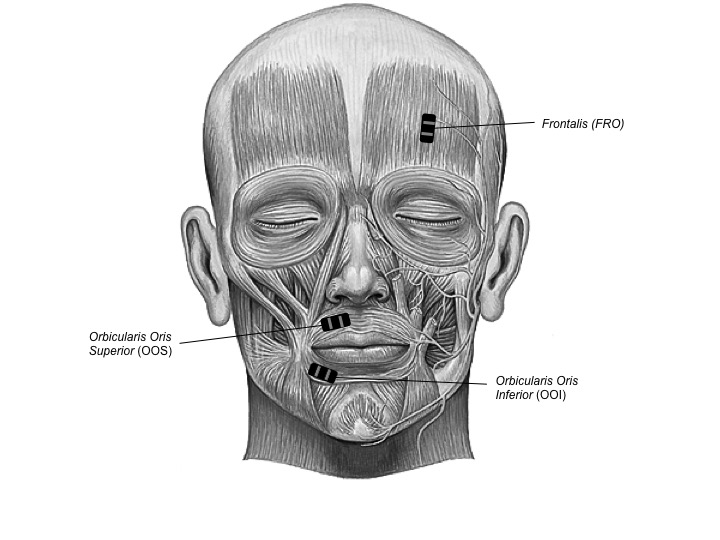
\includegraphics{assets/face_emg} 

}

\caption{Facial muscles of interest. Two speech-related labial muscles: orbicularis oris superior (OOS) and orbicularis oris inferior (OOI); as well as one non speech-related but sadness-related facial muscle: frontalis (Front).}\label{fig:unnamed-chunk-1}
\end{figure}

\subsection{Procedure}\label{procedure}

This study consisted of two parts. The first part was carried out a week
before the EMG experiment and consisted in checking the inclusion
criteria. We checked that participants did not exceed a threshold on a
depressive symptoms scale. This was assessed using the French version of
the Center for Epidemiologic Studies Depression scale (CES-D; Fuhrer \&
Rouillon, 1989), which evaluates the level of depres- sive symptom in
subclinical population. We also collected information about any
potential speech, neurologic, neuromuscular or cardiac disorders and
about academic curriculum. Finally, the tendency to ruminate (i.e.,
trait rumination) in daily life was evaluated using the French version
of the Mini-CERTS (Cambridge-Exeter Repetitive Thought Scale; Douilliez,
Philippot, Heeren, Watkins, \& Barnard, 2014). The second part included
two EMG interdependent experiments related to Rumination Induction and
Rumination Reduction by Muscle Relaxation. Specifically, Experiment 1
consisted of acquiring physiolo- gical EMG data during rest and induced
rumination and Experiment 2 consisted of acquiring physiological EMG
data after different kinds of relaxation (see below).

During both Experiment 1 and Experiment 2, momentary rumination was
assessed using four different Visual Analogue Scales (VAS, the first two
being adapted and translated to French from Huffziger, Ebner- Priemer,
Koudela, Reinhard, \& Kuehner, 2012) rated from 0 to 100: i) ``At this
moment, I am thinking about my feelings'' (referred to as VAS
``Feelings''), ii) ``At this moment, I am thinking about my problems''
(referred to as VAS ``Problems''), iii) ``At this moment, I am brooding
about negative things'' (referred to as VAS ``Brooding'') and iv) ``At
this moment, I am focused on myself'' (referred to as VAS ``Focused'').

\subsubsection{Experiment 1: rumination
induction}\label{experiment-1-rumination-induction}

Participants were seated in front of a computer screen in a comfortable
and quiet room. EMG sensors were positioned as explained above (see Fig.
1). Before the rumination induction, each participant underwent a
non-specific relaxation session (i.e., without targeting specific
muscles) in order to minimize inter-individual initial thymic
variability (approximate duration ∼330 s). Immediately after, partici-
pants were instructed to remain silent and not to move for one minute to
carry out EMG ``baseline'' measurements. Then, participants' initial
level of rumination was assessed using the four VASs.

Subsequently, participants were invited to perform a 15-min I.Q. test,
which was presented on the computer screen facing them. They were
instructed to correctly respond to three types of I.Q. questions
(logical, mathematical and spatial-reasoning questions) in a very short
time (30 s). Most of the questions were very difficult, if not
impossible, to correctly answer in 30 s. We included ten different
questions for each of the three types of IQ question: ten logical
questions (e.g., finding the next number of a Fibonacci sequence), ten
mathematical questions (e.g., ``What is the result of the following
calculus: (30/165) − (70/ 66)'') and ten spatial-reasoning questions
(e.g., finding the next figure of a series). Forced-failure tasks have
extensively been employed in the literature to induce a slightly
negative mood, ideal for subsequent rumination induction (e.g., LeMoult
\& Joormann, 2014; Van Randenborgh, Hüffmeier, LeMoult, \& Joormann,
2010).

After the I.Q. test, participants were invited to reflect upon the
causes and consequences of their feelings, during five minutes (rumina-
tion induction). This method is based on the induction paradigm
developed by Nolen-Hoeksema and Morrow (1993). The classical paradigm
uses a series of prompts. In order to avoid the potential confound in
muscle activity induced by silent reading, we did not use the full
paradigm. We simply summarised the series of prompts by one typical
induction sentence. During this period, participants were asked to
remain silent and not to move, while EMG recordings were carried out
(i.e., EMG Post-induction measures). EMG signals of rumination were
collected during the last minute of this period. Finally, partici- pants
were instructed to self-report momentary rumination on the four VASs.

\subsubsection{Experiment 2: rumination reduction by
relaxation}\label{experiment-2-rumination-reduction-by-relaxation}

After Experiment 1, participants were randomly allocated to one of three
groups. In the first group, participants listened to a pre-recorded
relaxation session that was focused on orofacial speech-related muscles
(``Orofacial Relaxation'' condition). In the second group, relaxation
was focused on the arm muscles (``Arm Relaxation'' condition). In the
third group, participants simply listened to a story, read by the same
person, for an equivalent duration (``Story'' condition, detailed
content of the story can be found in the Supplementary Materials, in
French). In summary, the first condition allowed us to evaluate the
effects of targeted speech muscle relaxation on rumination. The second
condition allowed evaluating the effects of a non-orofacial relaxation
(i.e., speech- unrelated muscles) while the third condition allowed
controlling for effects of attentional distraction during relaxation
listening.

The speeches associated with the three conditions, relaxation sessions
and story listening session, were delivered to the participants through
loudspeakers. They were recorded by a professional sophrology therapist
in an anechoic room at GIPSA-lab (Grenoble, France) and were
approximately of the same duration (around 330 s).

After the relaxation/distraction session, participants were asked to
remain silent and not to move during one minute, during which EMG
measurements were collected (EMG Post-relaxation measures). Finally,
participants were instructed to self-report rumination on the four VASs.

\subsection{Data processing and
analysis}\label{data-processing-and-analysis}

\subsubsection{EMG data processing}\label{emg-data-processing}

EMG signal pre-processing was carried out using Labchart 8. The EMG data
were high-pass filtered using a Finite Impulse Response (FIR) filter at
a cut-off of 20 Hz, using the Kaiser window method with β = 6. Then,
output of this first filter was to a low-pass filtered at a cut-off of
450 Hz (with the same parameters), in order to focus on the 20--450 Hz
frequency band, following current recommendations for facial EMG studies
(DeLuca, 1997; DeLuca, Gilmore, Kuznetsov, \& Roy, 2010; Van Boxtel,
2001).

Although we specifically asked participants to remain silent and not to
move during EMG data collection, tiny facial movements (such as biting
one's lips) or vocal productions sometimes occurred. Periods with such
facial movement or vocal production were excluded from the analysis. To
do this, visual inspection of audio, video, and EMG signal was
performed. Specifically, for the EMG signals, we compared two methods of
signal selection. The first one consisted of setting a threshold on the
absolute value of the EMG signal and portions of signals above this
threshold were removed. This threshold was empiri- cally chosen using
visual inspection of a few samples and set to the mean EMG value plus 6
SDs. The second method consisted of manually removing periods of time
that included visually obvious bursts of EMG activity, corresponding to
overt contraction (as in Rapin et al., 2013). Based on samples from a
few participants, the comparisons between these two methods showed that
the automatic threshold method was somewhat less sensitive to overt
movements. Therefore, the second method was used, as it was more
conservative and less prone to leave data related to irrelevant overt
movements.

After pre-processing, EMG data were exported from Labchart soft- ware to
Matlab r2014a (Version 8.3.0.532, www.mathworks.fr). For each EMG
signal, mean values were computed under Matlab, using 200 ms sliding
windows. The average of these mean values were calculated for each
recording session (baseline, after induction and after
relaxation/induction). This provided a score for each muscle of interest
(OOS, OOI, FCR, FRO) in each Session (Baseline, Post- Induction,
Post-Relaxation) for each participant\footnote{Because of constraints
  attributable to the design of our experiment, we were not able to
  perform conventional control measures (e.g., time of the day, food
  consumption, sport activity, smoking habits, etc.). Moreover, in our
  study, periods of signal recording had to be shorter than usual HRV
  analysis time periods (cf.~methodology section). Although recent
  studies suggest that ``ultrashort term'' HRV analysis seems to
  correlate quite well with HRV analysis performed on longer periods of
  time (Brisinda et al., 2013; Salahuddin, Cho, Gi Jeong,\&Kim, 2007),
  we cannot exclude that our measurements might be unreliable. For these
  reasons, we chose not to present HRV results in this report and to
  focus on EMG results as well as subjective reports of rumination.}.

\subsubsection{Statistical analyses}\label{statistical-analyses}

Absolute EMG values are not meaningful as muscle activation is never
null, even in resting conditions, due in part to physiological noise
(Tassinary, Cacioppo, \& Vanman, 2007). In addition, there are inter-
individual variations in the amount of EMG activity in the baseline. To
normalise for baseline activity across participants, we used a
differential measure and expressed EMG amplitude as a percentage of
baseline level (Experiment 1) or of post-induction level (Experiment 2).

To model EMG amplitude variations in response to the rumination
induction (Experiment 1) and relaxation (Experiment 2), we used a
bayesian multivariate regression model with the natural logarithm of the
EMG amplitude (expressed in\% of baseline level) as an outcome, in an
intercept-only model (in Experiment 1), and using Condition (Orofacial,
Arm or Story) as a categorical predictor in Experiment 2. We used the
same strategy (two multivariate models) to analyse VAS scores (expressed
in relative changes) along the two experiments.

These analyses were conducted using RStudio (RStudio Team, 2015) and the
brms package (Bürkner, in press), an R implementation of Bayesian
multilevel models that employs the probabilistic program- ming language,
Stan (Carpenter et al., 2016). Stan implements gradient- based Markov
Chain Monte Carlo (MCMC) algorithms (e.g., Hamilto- nian Monte-Carlo),
which allow yielding posterior distributions that are straightforward to
use for interval estimation around all parameters. Two MCMC simulations
(or ``chains'') were run for each model, including 100,000 iterations, a
warmup of 10,000 iterations, and a thinning interval of 10. Posterior
convergence was assessed examining autocorrelation and trace plots, as
well as the Gelman-Rubin statistic. Fixed effects were estimated via the
posterior mean and 95\% highest density intervals (HDIs), where an HDI
interval is the Bayesian analogue of a classical confidence
interval\footnote{While not suffering from the misunderstandings
  associated with frequentist confidence intervals (for more details,
  see for instance Morey, Hoekstra, Rouder, Lee \& Wagenmakers, 2015).}.

This strategy allowed us to examine posterior probability distribution
on each parameter of interest (i.e., effects of session and condition on
each response variable). When applicable, we also report evidence ratios
(ERs), computed using the hypothesis function of the brms package
(Bürkner, in press). These evidence ratios are simply the posterior
probability under a hypothesis against its alternative (Bürkner, in
press). We also report summary statistics (mean and HDI) of Cohen's d
effect sizes, computed from the posterior samples.

\section{Results}\label{results}

\subsection{Experiment 1: rumination
induction}\label{experiment-1-rumination-induction-1}

The evolution of VAS scores (for the four assessed scales: Feelings,
Problems, Brooding, and Focused) and EMG (for the four muscles: OOS,
OOI, FCR and FRO) activity from baseline to post-induction were
examined.

\subsubsection{Self-reported rumination measures: VAS
scores}\label{self-reported-rumination-measures-vas-scores}

Results for VAS relative changes based on the multivariate models
described earlier are shown in the right panel of Fig. 2. Thereafter,
\(\alpha\) represents the mean of the posterior distribution of the
intercept. Raw pre- and post-induction scores are provided in
Supplementary Materials.

Mean VAS score on the Feelings scale was slightly lower after induction
(\(\alpha\) = −5.55, 95\% HDI {[}-10.89, −0.24{]}, d = −0.23, 95\% HDI
{[}-0.46, −0.01{]}), while Problems score was slightly higher
(\(\alpha\) = 3.99, 95\% HDI {[}-2.04, 9.83{]}, d = 0.15, 95\% HDI
{[}-0.08, 0.37{]}). We observed a strong increase of the score on the
Brooding scale (\(\alpha\) = 14.45, 95\% HDI {[}8.07, 20.72{]}, d =
0.50, 95\% HDI {[}0.26, 0.74{]}), and a strong decrease on the Focused
scale (\(\alpha\) = −11.63, 95\% HDI {[}-17, −6.07{]}, d = −0.48, 95\%
HDI {[}-0.72, −0.24{]}). As we examined the fit of the intercept-only
model, these estimates represent the posterior mean for each muscle.

In the following, we report the mean (indicated by the Greek symbol ρ)
and the 95\% HDI of the posterior distribution on the correlation
coefficient (\(\rho\)). Examination of the correlation matrix estimated
by the multivariate model revealed no apparent correlation neither
between Feelings and Problems scales (\(\rho\) = −0.01, 95\% HDI
{[}-0.23, 0.22{]}), nor between Feelings and Brooding (\(\rho\) = 0.08,
95\% HDI {[}-0.15, 0.30{]}). However, we observed a strong positive
correlation between Problems and Brooding VASs (\(\rho\) = 0.64, 95\%
HDI {[}.49, 0.76{]}), a positive correlation between Feelings and
Focused (\(\rho\) = 0.30, 95\% HDI {[}.08, 0.50{]}), and a negative
correlation between Problems and Focused (\(\rho\) = −0.30, 95\% HDI
{[}-0.49, −0.08{]}), as well as between Brooding and Focused (\(\rho\) =
−0.18, 95\% HDI {[}-0.39, 0.05{]}).

\begin{figure}

{\centering 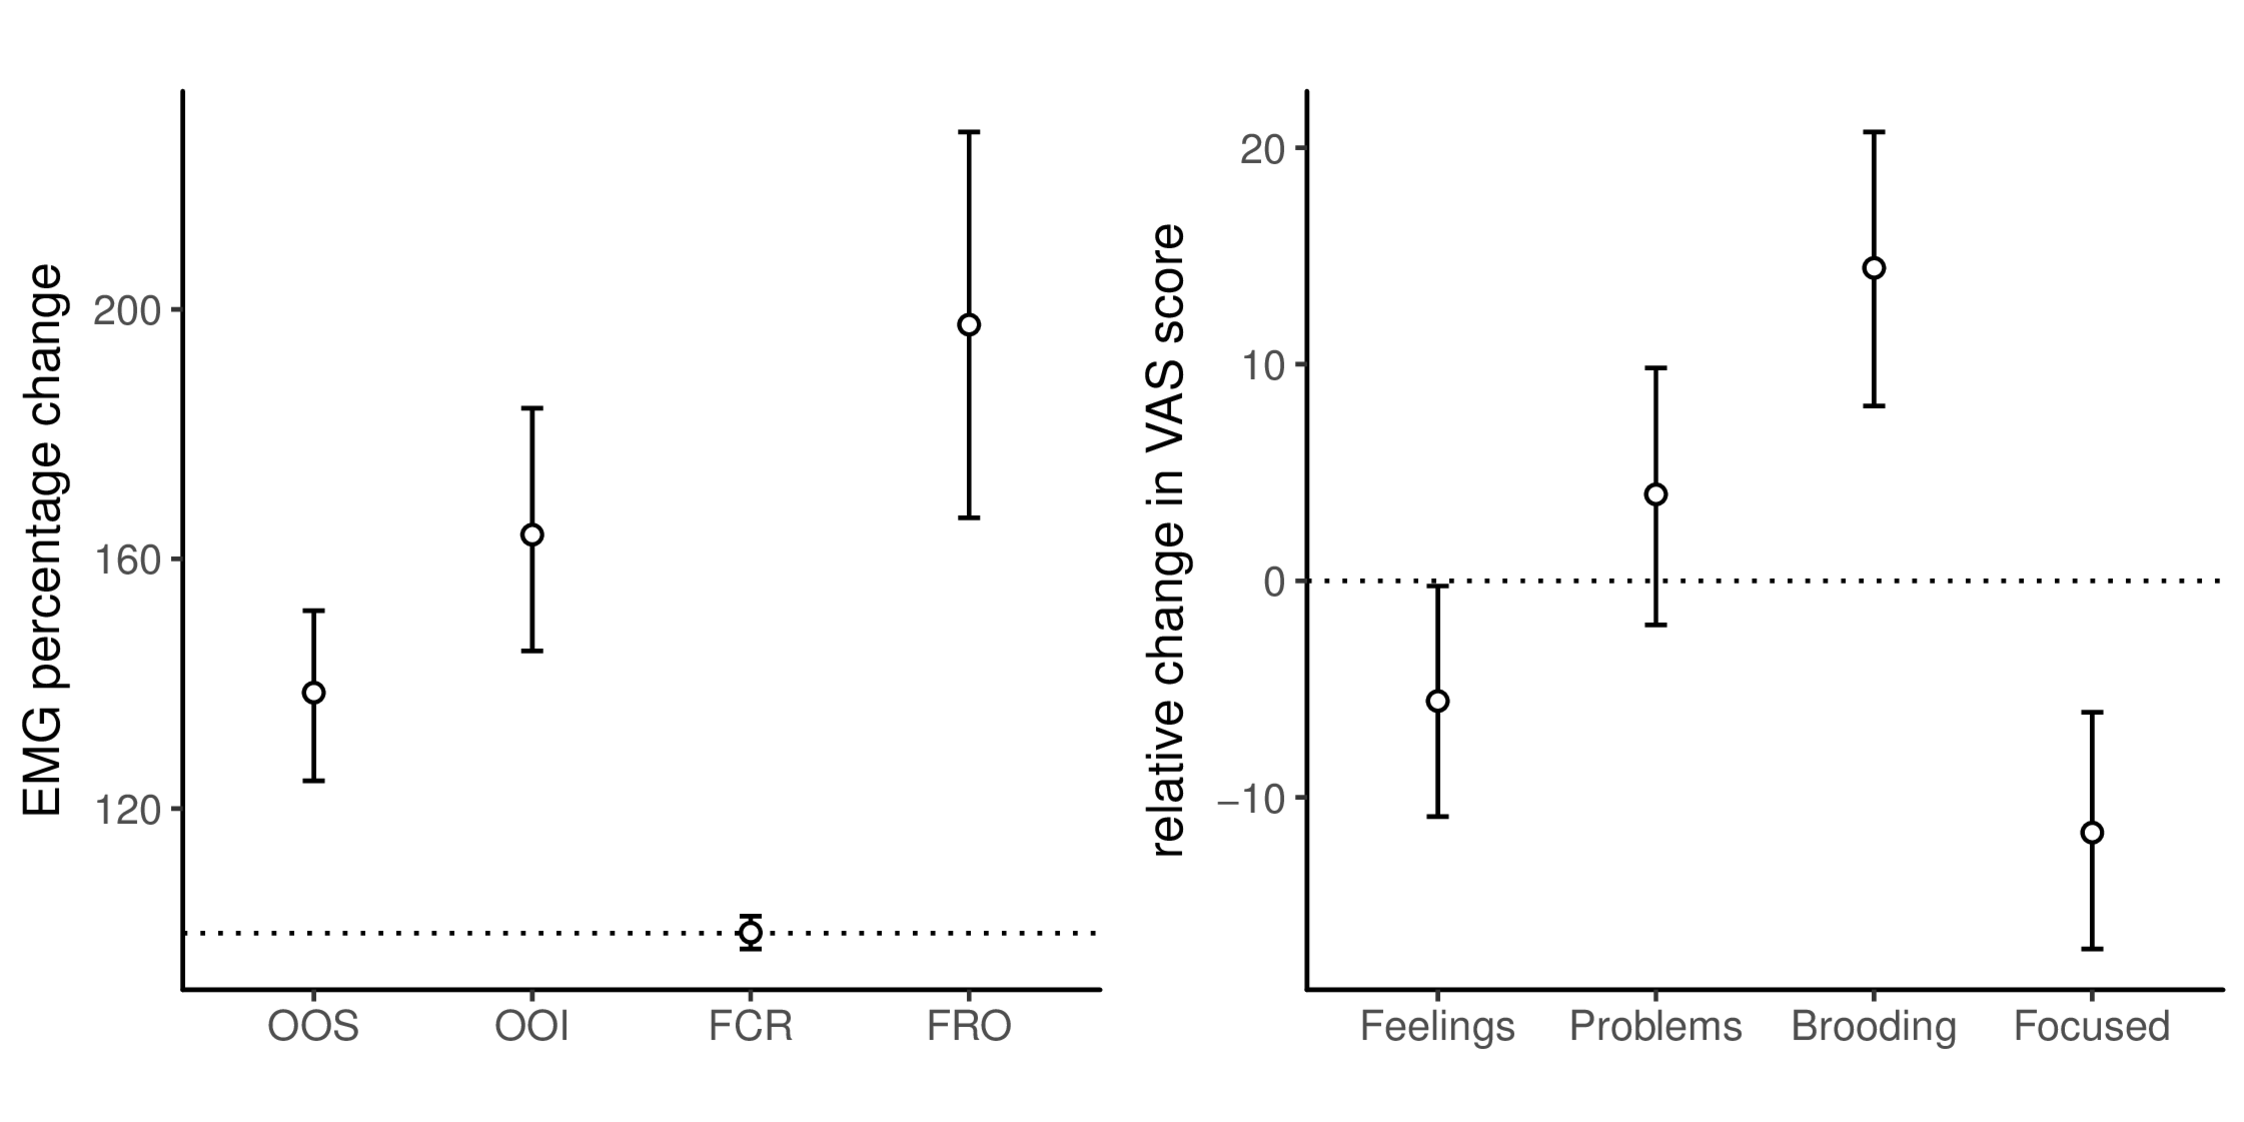
\includegraphics{assets/emg_fig1} 

}

\caption{Posterior mean (white dots) and 95\% credible intervals for the EMG amplitude (expressed in percentage of baseline level, left panel), and the VAS score (expressed in relative change from baseline, right panel). N = 71 (for each muscle and each VAS). Dashed line represents the null value (i.e., 100).}\label{fig:unnamed-chunk-2}
\end{figure}

\subsubsection{EMG}\label{emg}

Results for EMG data based on the multivariate model described earlier
are shown in the left panel of Figure 2. Summary statistics were
computed on posterior samples transformed back from log scale.

Mean EMG amplitude for OOS was higher after induction (\(\alpha\) =
138.57, 95\% HDI {[}124.43, 151.71{]}, d = 0.66, 95\% HDI {[}0.49,
0.84{]}) as well as for OOI (\(\alpha\) = 163.89, 95\% HDI {[}145.24,
184.14{]}, d = 0.77, 95\% HDI {[}0.61, 0.94{]}), and FRO (\(\alpha\) =
197.55, 95\% HDI {[}166.59, 228.42{]}, d = 0.74, 95\% HDI {[}0.59,
0.89{]}). Effects on the FCR were approximately null (\(\alpha\) =
100.10, 95\% HDI {[}97.48, 102.76{]}, d = 0.01, 95\% HDI {[}-0.24,
0.23{]}).

Examination of the correlation matrix estimated by the bayesian
multivariate model revealed a positive correlation between OOS and OOI
EMG amplitudes (\(\rho\) = 0.44, 95\% HDI {[}.24, 0.61{]}), while no
apparent correlations neither between OOS and FCR (\(\rho\) = 0.09, 95\%
HDI {[}-0.14, 0.31{]}), OOS and FRO (\(\rho\) = 0.12, 95\% HDI {[}-0.11,
0.35{]}), OOI and FCR (\(\rho\) = 0.02, 95\% HDI {[}-0.21, 0.25{]}), FRO
and FCR (\(\rho\) = −0.06, 95\% HDI {[}-0.28, 0.17{]}), nor OOI and FRO
(\(\rho\) = 0.07, 95\% HDI {[}-0.16, 0.29{]}). Scatterplots, marginal
posterior distributions and posterior distributions on correlation
coefficients are available in Supplementary Materials (Supplementary
materials, data, reproducible code and figures are available at:
\url{https://osf.io/882te/}).

In order to check whether the propensity to ruminate could predict the
effects of the rumination induction on EMG amplitude, we compared the
multivariate model described above, with a similar model but with the
score on the abstract dimension of the Mini- CERTS as an additional
predictor. We compared these models using the widely applicable
information criterion (WAIC; Watanabe, 2010), via the WAIC function of
the brms package (Bürkner, in press). Results showed that the
intercept-only model had a lower WAIC (WAIC = 177.39) than the more
complex model (WAIC = 182.01), indicating that there is no predictive
benefit in adding the Mini-CERTS score as a predictor.

\subsubsection{Correlations between EMG amplitudes and VAS
scores}\label{correlations-between-emg-amplitudes-and-vas-scores}

Correlations between EMG amplitudes and VAS scores were exam- ined using
the BayesianFirstAid package (Bååth, 2013), using 15,000 iterations for
each correlation coefficient. Both estimated correlation coefficients
(\(\rho\)s) and 95\% HDIs are reported in Table 1.

\subsection{Experiment 2: rumination reduction by
relaxation}\label{experiment-2-rumination-reduction-by-relaxation-1}

In the second experiment, we aimed at comparing the evolution in EMG
activity and VAS scores from post-induction to post-relaxation in three
different conditions: Orofacial relaxation, Arm relaxation, and
listening to a Story.

\subsubsection{Self-reported rumination measures: VAS
scores}\label{self-reported-rumination-measures-vas-scores-1}

Posterior means and 95\% HDIs of the VAS scores in each condition of
experiment 2 are represented in Fig. 3 and Table 1 (Table 2).

In order to compare the effects of the two kind of relaxation on the VAS
scores, we then used the hypothesis function of the brms package that
allows deriving evidence ratios (ER). These evidence ratios are simply
the posterior probability under a hypothesis (e.g., the hypothesis that
the Orofacial relaxation session would be more effective in reducing
self-reported rumination than the Arm relaxation session) against its
alternative (Bürkner, in press).

Since the Problems and the Brooding scales seemed to be sensitive
markers of rumination (as their scores increased after induction in
Experiment 1), our analyses were focused on these two scales.

Concerning the Problems VAS, the decrease observed in the Orofacial
condition was more pronounced than in the Arm condition (Est = −11.06,
SE = 6.35, ER10 = 22.65), and slightly more pro- nounced compared to the
Story condition (Est = −6.05, SE = 6.31, ER10 = 4.98). The observed on
the Brooding VAS score in the Orofacial condition was larger than in the
Arm condition (Est = −9.98, SE = 6.07, ER10 = 18.85), and slightly more
important compared to the Story condition (Est = −5.23, SE = 6.01, ER10
= 4.27).

\begin{figure}

{\centering 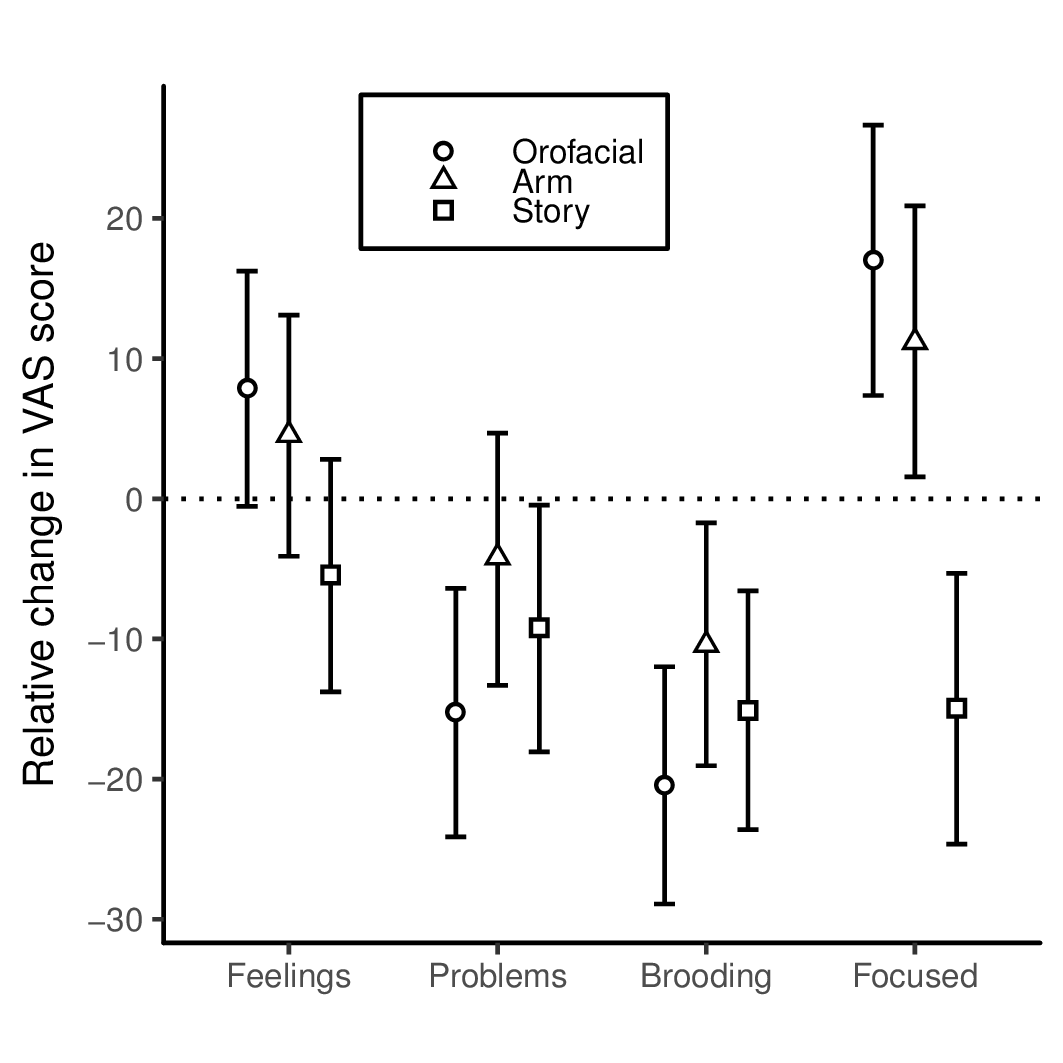
\includegraphics{assets/emg_fig2} 

}

\caption{Posterior mean and 95\% credible intervals for the VAS score (expressed in relative change from post-induction level).}\label{fig:unnamed-chunk-3}
\end{figure}

\subsubsection{EMG}\label{emg-1}

Posterior means and 95\% HDIs of the EMG amplitude in each condition of
experiment 2 are represented in Figure XX and reported in Table XX.

We used the same strategy as before to compare the effects of the two
kinds of relaxation on the EMG amplitudes.

Concerning the OOS, the observed decrease in the Orofacial condition was
more pronounced than in the Arm condition (Est = −0.34, SE = 0.14, ER10
= 140.73), as well as concerning the OOI (Est = −0.35, SE = 0.19, ER10 =
29.46), while we observed no noticeable differences between the two
kinds of relaxation concerning the EMG amplitude of the FRO (Est =
-0.04, SE = 0.14, ER10 = 1.53).

\begin{figure}

{\centering 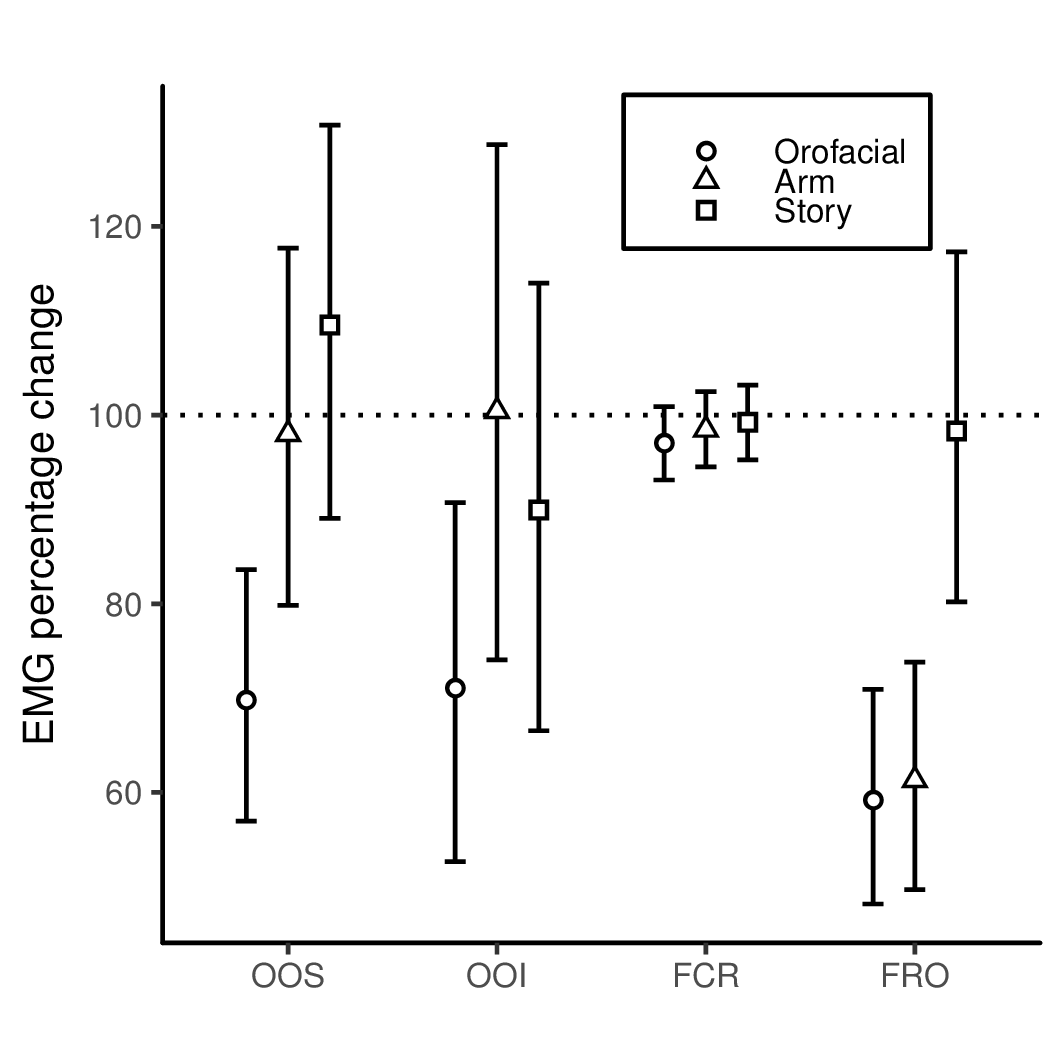
\includegraphics{assets/emg_fig3} 

}

\caption{Posterior mean and 95\% credible intervals for the VAS score (expressed in relative change from post-induction level).}\label{fig:unnamed-chunk-4}
\end{figure}

\section{Discussion}\label{discussion}

\subsection{Experiment 1}\label{experiment-1}

In the first experiment, we examined electromyographic correlates of
induced rumination in healthy individuals. According to the Motor
Simulation view, we predicted an increase in the activity of all facial
muscles after the rumination induction, associated with an increase in
self-reported rumination. Alternatively, the Abstraction view predicted
an increase in self-reported rumination associated with an increase in
forehead activity with no changes in either lip or forearm activity.

To test the predictions of these two theoretical views, we compared EMG
measures and VAS scores after induction to their values before
induction. EMG activity was examined in four muscles: OOS and OOI, two
muscles involved in speech production, FRO, a facial negative-
affect-related but not speech-related muscle, and FCR, a non-facial
control muscle on the non-dominant forearm.

As predicted by the Motor Simulation view, we observed an increase in
the activity of the two speech-related muscles (OOS \& OOI) as well as
in the negative-affect-related muscle (FRO) and no change in FCR
activity. The increase in facial EMG together with the increase in the
subjective reports of rumination suggests that facial EMG increase is a
correlate of verbal rumination. As supported by several studies results,
the forehead muscle activity has been associated with unpleasant
emotions (Jäncke et al., 1996) or anxiety (Conrad \& Roth, 2007). The
increase in FRO activity observed here is consistent with the increase
in negative emotions induced by our negatively valenced induction
procedure. Orbicularis oris lip muscles are associated with speech
production. The increase in lip activity observed here suggests that the
speech motor system was involved during the ruminative phase. The fact
that the FCR remained stable after rumination induction suggests that
the observed facial activity increase was not due to general body
tension induced by a negative mental state. These facial EMG results
therefore support the hypothesis that rumination is an instance of
articulatory-specified inner speech.

After the rumination induction, a larger increase in OOI activity was
observed compared to the increase in OOS activity. This finding is
consistent with previous findings of higher EMG amplitude in the lower
lip during speech and inner speech (e.g., Barlow \& Netsell, 1986;
Regalo et al., 2005; Sokolov, 1972) or auditory verbal hallucinations
(Rapin et al., 2013). Rapin et al. (2013) have explained the difference
between the activities of the two lip muscles by muscle anatomy. The
proximity of the OOI muscle with other speech muscles (such as the
depressor angular muscle or the mentalis) could increase the surface EMG
signal captured on the lower lip (OOI), as compared to the upper lip
(OOS) during speech. An even larger increase in FRO activity was
observed compared to the increase in lip muscle activity. As EMG
amplitude is known to vary with muscle length (Babault, Pousson,
Michaut, \& Van Hoecke, 2003), the greater increase in frontalis
activity could be explained by its anatomical properties.

However, although a functional distinction can be drawn between the
forehead and the lip muscles, one should acknowledge the fact that these
two sets of muscles can be commonly activated during some behaviours.
For instance, Van Boxtel \& Jessurun (1993) have shown that orbicularis
oris inferior and frontalis were both activated during a two-choice
serial reaction task in which nonverbal auditory or visual signals were
presented. Moreover, there was a gradual increase in EMG activity in
these muscles during the task, either when the task was prolonged or
when the task was made more difficult. They interpreted this increase in
EMG activity as associated with a growing compensa- tory effort to keep
performance at an adequate level. An alternative interpretation is that
the increase in task difficulty was dealt with by inner verbalization.
Covertly rehearsing the instructions or covertly qualifying the stimuli
might have helped the participants to perform adequately. Therefore, the
increase in orbicularis oris activity might have been related to an
increase in covert verbalization, whereas the increase in frontalis
activity might have been related to increased anxiety or tension. The
fact that the EMG increase was muscle specific, and that some facial
muscles (orbicularis oculi, zygomaticus major, temporalis) did not show
an increase in activity unless the task became too difficult, supports
this interpretation. It cannot be ruled out, however, that orbicularis
oris activity may in some cases be related to mental effort without
mental verbalisation. Nevertheless, although the IQ test itself was
designed to induce mental effort, no cognitively demanding task was
asked to the participant during the period of EMG recording (i.e.,
approximately four minutes after the end of the test). Although we
cannot absolutely exclude that rumination in itself could require
cognitive effort, it seems unlikely that mental effort was the main
factor of variation.

Scores on the VAS need to be discussed in further detail. We examined
which VAS scales were most suitable to capture changes in state
rumination to allow focused analyses. Due to the ``pre-baseline''
relaxation session, during which participants were asked to concentrate
on their body and breathing cycles, participants reported a high level
of attentional self-focus at baseline (``Feelings'' and ``Focused''
VAS). Because of the high level of self-focused attention at baseline,
it is likely that the scores on the ``Feelings'' and ``Focused'' VAS did
not show the expected increase after rumination induction (ceiling
effect). The scores on the scales ``Problems'' and ``Brooding'', which
are more representative of maladaptive rumination, did increase after
our rumination induction paradigm, however. Interestingly, the
``Brooding'' VAS corresponded to a larger increase and seemed to be more
sensitive to rumination induction than the ``Problems'' VAS. Given this
greater sensibility and the strong positive correlation between the
``Brooding'' and the ``Problems'' VAS, it thus make sense to consider
the ``Brooding'' VAS as a better estimate of ruminative state, at least
within our paradigm. We will therefore only use this scale to assess
rumination in the following.

The fact that we did not observe any association between the propensity
to ruminate (as measured by the Mini-CERTS questionnaire) and the
effects of the induction is consistent with the results of Rood,
Roelofs, Bögels, and Arntz (2012) who found that the level of trait
rumination did not moderate the effects of a rumination induction.

\subsection{Experiment 2}\label{experiment-2}

In the second experiment, we studied the effects of two muscle- specific
relaxation sessions: Orofacial relaxation and Arm relaxation. We
compared their effects to a third control condition (Story), which did
not involve the deliberate relaxation of any specific muscle. Our
predictions were that a decrease in facial EMG activity should be
observed in each condition. If the Motor Simulation view is correct, we
expected a larger decrease in the activity of all facial muscles in the
``Orofacial relaxation'' condition than in the ``Arm relaxation''
condition, associated with a larger decrease in self-reported
rumination. Additionally, we expected a more pronounced decrease in the
two relaxation conditions (orofacial and arm relaxation conditions) than
in the control (``Story'') condition. We also expected no difference
between relaxation conditions regarding the change in the forearm muscle
activity.

The data indicated a decrease in self-reported rumination (``Brooding''
VAS) in each condition. The ``Orofacial'' relaxation condi- tion
elicited a slightly larger decrease than the ``Arm relaxation'' or the
``Story'' condition. However, there was extensive individual variation
in response to these conditions. As concerns EMG results, we observed a
decrease in OOS and OOI activities in all three conditions but this
decrease was more pronounced in the orofacial condition than in the
other two conditions. The frontalis activity did not show the same
pattern. A similar FRO activity decrease was observed in both the
orofacial and the non-orofacial relaxation conditions. Therefore, in
Experiment 2, the lip muscles and the forehead muscle follow differ-
ential evolutions. A dissociation was observed: whereas both orofacial
and arm relaxations resulted in a decrease in forehead activity, only
orofacial relaxation was successful at reducing lip activity.

Considering both VAS results and the dissociation in EMG patterns,
several interpretations are possible. The first interpretation is that
verbal production associated with rumination was more reduced by
orofacial muscular relaxation than by non-orofacial relaxation. This
interpretation is consistent with the fact that the ``Brooding'' VAS was
slightly more decreased in this condition compared to the other two. The
larger decrease in OOS and OOI amplitude after orofacial relaxa- tion
would thus reflect this reduction in verbal production, as hypothesised
by the Motor Simulation view. The fact that FRO activity displayed a
similar decrease in both orofacial and non-orofacial relaxation
conditions could suggest that any means of body relaxation (be it
orofacial or not) is appropriate to reduce negative affect and can
therefore reduce forehead contraction. This suggests that the FRO
activity increase presumably reflected negative affect and tension (such
as observed in EMG studies on generalised anxiety disorder patients, see
Conrad \& Roth, 2007 for a review).

Alternatively, one could also argue that the larger decrease in lip
muscle activity after orofacial relaxation finds a more trivial explana-
tion in that it seems obvious to expect that orofacial relaxation will
be more efficient to reduce lip muscle contraction than non-orofacial
relaxation. Thus, the different impacts of the two relaxation sessions
on the lip muscles would not be related to reduced rumination per se but
simply to a more anatomically targeted relaxation. However, several
observations argue against such an interpretation. The larger decrease
in the ``Brooding'' VAS in the orofacial relaxation condition compared
with the other conditions suggests that the reduction in lip muscle
activity is indeed related to the reduction in rumination. Moreover, an
interpretation solely based on anatomical links does not explain why FRO
activity displayed the same amount of reduction in both relaxation
sessions. If reduction in muscle activity was merely related to the
effect of facial muscle relaxation, then the decrease in FRO activity
should have also been higher in the orofacial relaxation condition than
in the other relaxation condition, which was not the case. Therefore the
dissociation between forehead and lip patterns of activity, together
with the differential effects of the two types of relaxation on
subjective rumination reports strongly suggest that different processes
underlie the activity of these two sets of muscles. We therefore
consider that the first interpretation is more plausible: frontalis
activity seems related to overall facial tension due to negative affect
whereas lip activity seems to be related to the specific involvement of
the speech musculature in rumination. These results thus seem to confirm
the interpretation of decreased OOS and OOI activities in the orofacial
relaxation condition as markers of rumination reduction.

Interestingly, we observed no changes of forearm EMG activity in any of
the three conditions of experiment 2. The fact that the relaxation
session focused on the forearm was not associated with a decrease in FCR
activity has a simple explanation: FCR activity had not increased after
rumination induction and had remained at floor level. The forearm was
thus already relaxed and the Arm relaxation session did not modify FCR
activity. Another interesting conclusion related to this absence of
modification of forearm activity is that relaxation does not spuriously
decrease muscle activity below its resting level. One possible
interpretation of the increase in lip EMG after rumination induction
could have been that baseline relaxation artificially decreased baseline
activity under its resting level. The facts that forearm activity did
not decrease after arm-focused relaxation contradicts this
interpretation.

Finally, the ``Story'' condition was also associated with a decrease in
OOI and FRO activities. This could mean that listening to a story
reduced rumination to the same extent as relaxation did. However, the
discrepancy observed in ``Focused'' VAS between the two relaxation
conditions on the one hand and the control condition on the other hand,
suggests that the EMG decrease observed in the ``Story'' condition might
be attributable to a different cause than that observed in the two
relaxation conditions. Listening to a story could help reducing rumina-
tion by shifting attention away from ruminative thoughts. Relaxation
sessions could help reducing rumination by shifting attention to the
body in a beneficial way.

\subsection{General discussion}\label{general-discussion}

We set out two experiments to examine whether rumination involves motor
simulation or is better described as linguistically abstract and
articulatory impoverished. We used labial, facial, and arm EMG measures
to assess potential articulatory correlates of rumination. The patterns
of results of our study seem to be in favour of the motor nature of
verbal rumination. In Experiment 1, rumination induction was associated
with a higher score on the scale ``I am brooding about negative things''
which is representative of abstract- analytical rumination, considered
as verbal rumination. This maladap- tive rumination state was associated
with an increase in the activity of two speech-related muscles, without
modification of the arm muscle activity, which indicates that rumination
involves activity in speech articulatory muscles, specifically. The
concurrent increase in forehead muscle activity could be explained by an
increase in negative emotions induced by our negatively valenced
induction procedure. The results of Experiment 1 therefore show the
involvement of the speech muscula- ture during rumination. This is in
line with the Motor simulation view, according to which inner speech is
fully specified at the articulatory level, not just the lexical level.

In Experiment 2, guided relaxation resulted in a decrease in speech
muscle activity. In the lip muscles, the activity decrease was stronger
after orofacial relaxation than after arm-focused relaxation. In the
forehead muscle, however the effect was the same for both types of
relaxation. This decrease in speech muscle activity was associated with
a decrease in self-reports of rumination and was most pronounced after
orofacial relaxation. These findings suggest that a reduction in speech
muscle activity could hinder articulatory simulation and thus limit
inner speech production and therefore reduce rumination. This inter-
pretation is consistent with the Motor Simulation view of inner speech.
Brooding-type rumination was also diminished after the arm-focused
relaxation as well as after listening to a story, although less than in
the orofacial relaxation. This suggests that general relaxation or
distraction are also likely to reduce negative rumination. To summarize,
experi- ments 1 and 2 are consistent with the Motor Simulation view of
inner speech, according to which speech muscle activity is inherent to
inner speech production. Experiment 1 shows the involvement of the lip
musculature during brooding-type rumination. Experiment 2 suggests that
brooding-type rumination could be reduced by blocking or relaxing speech
muscles.

These data support the utility of labial EMG as a tool to objectively
assess inner speech in a variety of normal and pathological forms. We
suggest that this method could be used as a complement to self-report
measures, in order to overcome limitation of these measures.

Our results should be interpreted with some limitations in mind.
Firstly, our sample consisted exclusively of women. Although this
methodological choice makes sense considering the more frequent
occurrence of rumination in women, further studies should be con- ducted
to ascertain that our results may generalize to men. Secondly, in
Experiment 1, no between-subject control condition was used to compare
with the group of participants who underwent rumination induction. Thus,
we cannot rule out that other processes occurred between baseline and
rumination induction, influencing responding. Thirdly, substantial
inter-individual differences were observed concern- ing the size of the
effect of rumination induction on facial EMG activity. The results of
Jäncke (Jäncke, 1996; Jäncke et al., 1996) can shed light on this last
result. Jäncke used a similar procedure (i.e., negative mood induction
using a false I.Q. test and facial EMG measurements to assess emotions),
except that the experimenter was not in the room while participants
performed the test and acknowledged their results. The experimenter then
came back to the room and analysed participants' behaviours. Jäncke
observed an increase in facial muscular activity (assessed when
participants were reading their results) only in partici- pants who were
prone to express their distress when the experimenter came back, while
more introverted participants did not show any increased facial activity
when reading their results. Jäncke interpreted these results in the
framework of an ecological theory of facial expression, suggesting that
facial expressions would not only be guided by underlying emotions, but
also by their communicative properties. Considering these results, it
seems likely that the proneness of participants to communicate their
emotions could have mediated effects of the induction on their facial
EMG activity. This could partially explain the observed inter-individual
variability in facial EMG activity associated with rumination. Moreover,
even though rumination is a predominantly verbal process, one cannot
exclude that some of our participants experienced rumination in another
modality (e.g., ima- gery-based rumination), which would explain their
lower than average lip activity.

Thus, a logical next step is to examine qualitative factors that mediate
the link between rumination and facial muscular activity. These factors
(among others) could be proneness to communicate emotion or proneness to
verbalize affects. Additionally, recent studies suggest a link between
verbal aptitudes and propensity to ruminate. Uttl, Morin and Hamper
(2011) have observed a weak but consistent correlation between the
tendency to ruminate and scores on a verbal intelligence test. Penney,
Miedema and Mazmanian (2015) have observed that verbal intelligence
constitutes a unique predictor of rumination severity in chronic anxious
patients. To our knowledge, the link between verbal intelligence and
induced rumination has never been studied. It would be interesting to
examine whether the effects of a rumination induction could be mediated
by verbal intelligence, and to what extent this could influence related
facial EMG activity.

In conclusion, this study provides new evidence for the facial
embodiment of rumination, considered as a particular instance of inner
speech. Even if more data are needed to confirm these preliminary
conclusions, our results seem to support the Motor Simulation view of
inner speech production, manifested as verbal rumination. In addition,
facial EMG activity provides a useful means to objectively quantify the
presence of verbal rumination.

\section{Acknowledgements}\label{acknowledgements}

This project was funded by the ANR project INNERSPEECH {[}grant number
ANR-13-BSH2-0003-01{]}. The first author of the manuscript is funded by
a fellowship from Université Grenoble Alpes and a grant from the Pôle
Grenoble Cognition. We thank Nathalie Vallet for recording the
relaxation and distraction sessions. We thank our colleagues from
GIPSA-lab: Marion Dohen for her help in the recording of the audio
stimuli in the anechoic room at GIPSA-lab, as well as Christophe
Savariaux and Coriandre Vilain for their advice in the audio setup
associated with the EMG measures. We are also grateful to Rafael
Laboissière and Adeline Leclercq Samson for their advice concerning data
analysis. We sincerely thank two anonymous reviewers for their critical
reading of our manuscript and their many insightful comments and
suggestions. Access to the facility of the MSH-Alpes SCREEN platform for
conducting research is gratefully acknowledged.

\section{Supplementary data}\label{supplementary-data}

Supplementary data associated with this article can be found, in the
online version, at
\url{http://dx.doi.org/10.1016/j.biopsycho.2017.04.013}.

\chapter{Dissociating facial electromyographic correlates of visual and
verbal induced
rumination}\label{dissociating-facial-electromyographic-correlates-of-visual-and-verbal-induced-rumination}

Second EMG study with Sonja\ldots{}

\chapter{Zygoto experiment}\label{zygoto-experiment}

\ldots{}

\chapter{Articulatory suppression effects on induced
rumination}\label{articulatory-suppression-effects-on-induced-rumination}

Summary of the research\ldots{}\footnote{This experimental chapter is a
  manuscript reformatted for the need of this thesis. Source: The
  manuscript has been submitted to Psychological Research.
  Pre-registered protocol, preprint, data, as well as reproducible code
  and figures are available at: \url{https://osf.io/3bh67/}.}

\section{Introduction}\label{introduction-1}

A large part of our inner experience involves verbal content, with
internal monologues and conversations. Inner speech is considered as a
major component of conscious experience and cognition
\citep{Hubbard2010, Klinger1987, Hurlburt2013}. An important issue
related to inner speech concerns its format and nature and whether it is
better described as a mere evocation of abstract amodal verbal
representations or as a concrete motor simulation of actual speech
production. In the first case, inner speech is seen as divorced from
bodily experience, and includes, at most, faded auditory
representations. In the second case, inner speech is considered as a
physical process that unfolds over time, leading to an enactive
re-creation of auditory a well as articulatory percepts. The latter
hypothesis is interesting in the context of persistent negative and
maladaptive forms of inner speech, such as rumination. If this
hypothesis is correct, we could expect rumination --as a particular type
of inner speech-- to be disrupted by concurrent involvement of the
speech muscles.

\subsection{Multisensory and motor components of inner
speech}\label{multisensory-and-motor-components-of-inner-speech}

Introspective explorations of the characteristics of inner speech have
led to different views on the relative importance of its auditory and
articulatory components, and on the involvement of motor processes. For
\citet{Stricker1880}, ``speech representations are motor
representations'', while \citet{Egger1881} believed that auditory
representations are dominant in inner speech and that motor
representations are not always present. However, as noted by
\citet{Ballet1886}, these contradictory hypotheses might stem from an
over-generalization of their own introspective findings, the former
discovering motor feelings and the latter auditory images
\citep{Ballet1886}. In the same vein, \citet{Paulhan1886} claimed that
inner speech involves both auditory and motor images, defining motor
images as the sensations in the speech organs (larynx, tongue, lips)
that sometimes accompany inner speech. Therefore, Paulhan's notion of
\emph{motor images} are in fact related to somatosensory representations
rather than to the involvement of actual speech movements (as claimed by
Stricker). It remains, however, that a distinction was introduced by
19th century authors between sensory and motor phenomena in inner
speech, with sensory phenomena including auditory as well as
articulatory (or somatosensory) percepts. The intuitive distinction
between auditory and motor phenomena is referred to in contemporary
research by the terms of \emph{inner ear} and \emph{inner voice}, in
line with Baddeley's classic model of working memory
\citetext{\citealp[e.g.,][]{Baddeley1974}; \citealp[see
also][]{Buchsbaum2013}}. Baddeley's model relies on a partnership
between an \emph{inner ear} (i.e., storage) and an \emph{inner voice}
\citep[i.e., subvocal rehearsal; see][]{Smith1995}.

Empirical arguments supporting the crucial role of the inner voice in
verbal memory (subvocal rehearsal) and auditory imagery can be found in
studies using articulatory suppression, in which the \emph{action}
component (i.e., the \emph{inner voice}) of inner speech is disrupted.
Articulatory suppression usually refers to a task which requires
participants to utter speech sounds (or to produce speech gestures
without sound), so that this activity disrupts ongoing speech production
processes. Articulatory suppression can be produced with different
degrees of vocalisation, going from overt uttering of irrelevant words,
to whispering, mouthing (i.e., silent articulation), and simple clamping
of the speech articulators. Many verbal working memory studies have
shown that articulatory suppression impairs recall performance
\citep[e.g.,][]{Baddeley1984}.

In a study aiming at investigating the role of \emph{covert enactment}
in auditory imagery, \citet{Reisberg1989} observed that the verbal
transformation effect \citep[VTE,][]{Warren1958}, namely the alteration
of speech percepts when certain speech sounds are uttered in a
repetitive way, also occurred during inner speech (although the VTE was
smaller than during overt speech), but was suppressed by concurrent
articulation (e.g., chewing) or clamping the articulators. The fact that
the VTE was observed during inner speech and that it was reduced by
concurrent chewing, even in inner speech, speaks in favour of the view
of inner speech as an enacted simulation of overt speech.

Another piece of evidence for the effect of articulatory suppression on
inner speech comes from a recent study by \citet{Topolinski2009} on the
mere exposure effect, namely the fact that repeated exposure to a
stimulus influences the evaluation of this stimulus in a positive way
\citep{Zajonc1968}. Topolinski and Strack's study showed that the mere
exposure effect for visually presented verbal material could be
completely suppressed by blocking subvocal rehearsal (i.e., inner
speech) when asking participants to chew a gum. The effect was
preserved, however, when participants kneaded a soft ball with their
hand \citep{Topolinski2009}. This finding suggests that blocking speech
motor simulation interfered with the inner rehearsal of the visually
presented verbal stimuli, thereby destroying the positive exposure
effect. It provides additional experimental support to the view that
inner speech involves a motor component.

The occurrence of motor simulation during inner speech is further backed
by several studies using physiological measures to evaluate inner speech
production properties. Using electrodes inserted in the tongue tip or
lips of five participants, \citet{Jacobson1931} was able to detect
electromyographic (EMG) activity during several tasks requiring inner
speech. Similarly, \citet{Sokolov1972} recorded intense lip and tongue
muscle activation when participants had to perform complex tasks that
necessitated substantial inner speech production (e.g., problem
solving). Another study using surface electromyography (sEMG)
demonstrated an increase in activity of the lip muscles during silent
recitation tasks compared to rest, but no increase during the
non-linguistic visualisation task \citep{Livesay1996}. An increase in
the lip and forehead muscular activity has also been observed during
induced rumination \citep{Nalborczyk2017}. Furthermore, this last study
also suggested that speech-related muscle relaxation was slightly more
efficient in reducing subjective levels of rumination than non
speech-related muscle relaxation, suggesting that relaxing or inhibiting
the speech muscles could disrupt rumination.

\subsection{Rumination}\label{rumination}

Rumination is a ``class of conscious thoughts that revolve around a
common instrumental theme and that recur in the absence of immediate
environmental demands requiring the thoughts'' \citep{Martin1996}.
Despite the fact that depressed patients report positive metacognitive
beliefs about ruminating, which is often seen as a coping strategy in
order to regulate mood \citep[e.g.,][]{Papageorgiou2001}, rumination is
known to significantly worsen mood
\citep[e.g.,][]{Moberly2008, Nolen-hoeksema1993}, impair cognitive
flexibility \citep[e.g.,][]{Davis2000, Lyubomirsky1998}, and to lead
toward pronounced social exclusion and more interpersonnal distress
\citep{Lam2003}. Although partly visual, rumination is a predominantly
verbal process \citep{Goldwin2012, Mclaughlin2007} and can be considered
as a maladaptive type of inner speech.

In a study on worry, another form of repetitive negative thinking,
\citet{Rapee1993} observed a \emph{tendency} for articulatory
suppression, but not for visuo-spatial tasks, to produce some
interference with worrying. He concluded that worry involves the
phonological aspect of the central executive of working memory. We
further add that, since repeating a word seems to reduce the ability to
worry, this study suggests that articulatory aspects are at play during
worry.

In this context, the question we addressed in this study is whether
verbal rumination consists of purely abstract verbal representations or
whether it is better described as a motor simulation of speech
production, engaging the speech apparatus. If the latter hypothesis is
correct, rumination experienced in verbal form (in contrast to a
non-verbal form) should be disrupted by mouthing (i.e., silent
articulation), and should not be disrupted by a control task that does
not involve speech muscles (e.g., finger-tapping). Specifically, we thus
sought to test the hypotheses that rumination could be disrupted by
articulatory suppression (but not by finger-tapping), and that this
disruption would be more pronounced when rumination is experienced in a
verbal form than in a non-verbal form.

\section{Methods}\label{methods-1}

In the \emph{Methods} and \emph{Data analysis} sections, we report how
we determined our sample size, all data exclusions, all manipulations,
and all measures in the study \citep{Simmons2012}. A pre-registered
version of our protocol can be found on OSF:
\url{https://osf.io/3bh67/}.

\subsection{Sample}\label{sample}

We originally planned for 128 participants to take part in the study.
This sample size was set on the basis of results obtained by
\citet{Topolinski2009}, who observed an effect size around
\(\eta_{p}^{2}=.06\). We expected a similar effect size for the current
rumination disruption, since rumination can be conceived of as a subtype
of inner speech\footnote{In the original power calculations included in
  the OSF preregistration platform, we had inadequately specified the
  effect size in GPower, but we only realised this erroneous
  specification after the freezing of the preregistration on the OSF
  platform. Therefore, the current sample size slightly differs from the
  preregistered one.}.

As we anticipated drop-out of participants due to our inclusion criteria
(see below), a total of 184 undergraduate students in psychology from
the Université Grenoble Alpes took part in this experiment, in exchange
for course credits. They were recruited via mailing list, online student
groups, and posters. Each participant provided a written consent and
this study was approved by the local ethics committee (CERNI N°
2016-05-31-9). To be eligible, participants had to be between 18 and 35
years of age, with no history of motor, neurological, psychiatric, or
speech-development disorders. All participants spoke French as their
mother tongue. After each participant gave their written consent, they
completed the Center for Epidemiologic Studies - Depression scale
\citep[CES-D;][]{Radloff1977a}. The CES-D is a 12-item questionnaire,
validated in French \citep{Morin2011}, aiming to assess the level of
depressive symptoms in a subclinical population. Participants exceeding
the threshold of clinical depressive symptoms \citep[i.e.,
\textgreater{}23 for females and \textgreater{}17 for
males;][]{Radloff1977a} were not included in the study for ethical
reasons (N = 26).

To investigate articulatory suppression effects in the context of
rumination, a successful induction of rumination is a prerequisite.
Therefore, analyses were only conducted on participants who showed an
effect of the rumination induction (i.e., strictly speaking,
participants who reported more rumination after the induction than
before). We thus discarded participants who did not show any increase in
rumination level (N = 52, 32.91\% of total sample). The final sample
comprised 106 participants (Mean age = 20.3018868, SD = 2.5728064,
Min-Max = 18-31, 96 females).

\subsection{Material}\label{material-1}

The experiment was programmed with OpenSesame software
\citep{Mathot2012} and stimuli were displayed on a DELL latitude E6500
computer screen.

\subsubsection{Questionaires}\label{questionaires}

To control for confounding variables likely to be related to the
intensity of the induction procedure, we administered the French version
of the Positive and Negative Affect Schedule
\citep[PANAS;][]{Watson1988}, adapted to French by \citet{Gaudreau2006}.
This questionnaire includes 20 items, from which we can compute an
overall index of both positive (by summing the scores on 10 positive
items, thereafter \emph{PANASpos}) and negative affect (\emph{PANASneg})
at baseline. This questionnaire was administered at baseline. In order
to evaluate trait rumination, at the end of the experiment participants
completed the short version of the Ruminative Response Scale
\citep[RRS-R,][]{Treynor2003}, validated in French (Douilliez, Guimpel,
Baeyens, \& Philippot, \emph{in preparation}). From this questionnaire,
scores on two dimensions were analysed (\emph{RRSbrooding} and
\emph{RRSreflection}).

\subsubsection{Measures}\label{measures}

Measures of state rumination were recorded using a Visual Analogue Scale
(VAS) previously used in \citet{Nalborczyk2017}. This scale measured the
degree of agreement with the sentence ``At this moment, I am brooding on
negative things'' (translated from French), on a continuum between ``Not
at all'' and ``A lot'' (afterwards coded between 0 and 100). This scale
is subsequently referred to as the \emph{RUM} scale. It was used three
times in the experiment, at baseline (after training but before the
experiment started), after rumination induction, and after a motor task.

Additionally, participants answered questions about the modality of the
thoughts that occurred while performing the motor task. This last
questionnaire consisted of one question evaluating the occurrence
frequency of different modalities of inner thoughts (e.g., visual
imagery, verbal thoughts, music). Then, a verbal/non-verbal ratio (i.e.,
the score on the verbal item divided by the mean of the score on the
non-verbal items) was computed, hereafter referred to as the
\emph{Verbality} continuous predictor (this scale is available online:
\url{https://osf.io/3bh67/}).

\subsubsection{Tasks}\label{tasks}

In the first part of the experiment, ruminative thoughts were induced
using a classical induction procedure. Then a motor task was executed.
Participants were randomly allocated to one of two conditions. In the
\emph{Mouthing} condition, the task consisted of repetitively making
mouth opening-closing movements at a comfortable pace. This condition
was selected as it is commonly used in articulatory suppression studies
\citep[e.g.,][]{Baddeley1984}. As a control, a finger-tapping condition
was used (the \emph{Tapping} condition), that consisted of tapping on
the desk with the index finger of the dominant hand at a comfortable
pace.

Although finger-tapping tasks are generally considered as good control
conditions when using speech motor tasks, since they are comparable in
terms of general attentional demands, it may be that orofacial gestures
are intrinsically more complex than manual gestures \citep[i.e., more
costly,][]{Emerson2003}. To discard the possibility that orofacial
gestures (related to the \emph{Mouthing} condition) would be cognitively
more demanding than manual ones (related to the \emph{Tapping}
condition), we designed a pretest experiment in order to compare the two
interference motor tasks used in the main experiment. Results of this
control experiment showed no difference on reaction times during a
visual search task between the two interference tasks (i.e., mouthing
and finger-tapping). Full details are provided in Appendix A.

\subsection{Procedure}\label{procedure-1}

The experiment took place individually in a quiet and dimmed room. The
total duration of the session ranged between 35min and 40min. Before
starting the experiment, participants were asked to perform the motor
task during 1 min, while following a dot moving at a random pace on the
screen in front of them. This task was designed to train the
participants to perform the motor task adequately. Following this
training and after describing the experiment, the experimenter left the
room and each participant had to fill-in a baseline questionnaire
(adaptation of PANAS, see above) presented on the computer screen.
Baseline state rumination was then evaluated using the \emph{RUM} scale.
The whole experiment was video-monitored using a Sony HDR-CX240E video
camera, in order to check that the participants effectively completed
the task.

\subsubsection{Rumination induction}\label{rumination-induction}

Rumination induction consisted of two steps. The first step consisted of
inducing a negative mood in order to enhance the effects of the
subsequent rumination induction. Participants were asked to recall a
significant personal failure experienced in the past five years. Then,
participants were invited to evaluate the extent to which this memory
was ``intense for them'' on a VAS between ``Not at all'' and ``A lot'',
afterwards coded between 0 and 100, and referred to as \emph{Vividness}.

The second step consisted of the rumination induction proper. We used a
French translation of the \citet{Nolen-hoeksema1993} rumination
induction procedure. Participants had to read a list of 44 sentences
related to the meaning, the causes and the consequences of their current
affective or physiological state. Each phrase was presented on a
computer screen for 10 seconds and the total duration of this step was 7
minutes and 20 seconds. State rumination was then evaluated again using
the same VAS as the one used at baseline (\emph{RUM}).

\subsubsection{Motor task}\label{proc_supp}

After the rumination induction, participants were asked to continue to
think about ``the meaning, causes, and consequences'' of their feelings
while either repetitively making mouth movements (for participants
allocated in the ``Mouthing'' condition) or finger-tapping with the
dominant hand for five minutes (for participants allocated in the
``Tapping'' condition). Afterwards, state rumination was again evaluated
using the \emph{RUM} scale.

In order to evaluate trait rumination, participants completed the short
version of the RRS (see above). Then were filled in the questionnaire on
the modality of the thoughts that occurred while performing the motor
task (see above). Figure \ref{fig:diagram} summarises the full
procedure.

\begin{figure}[H]

{\centering 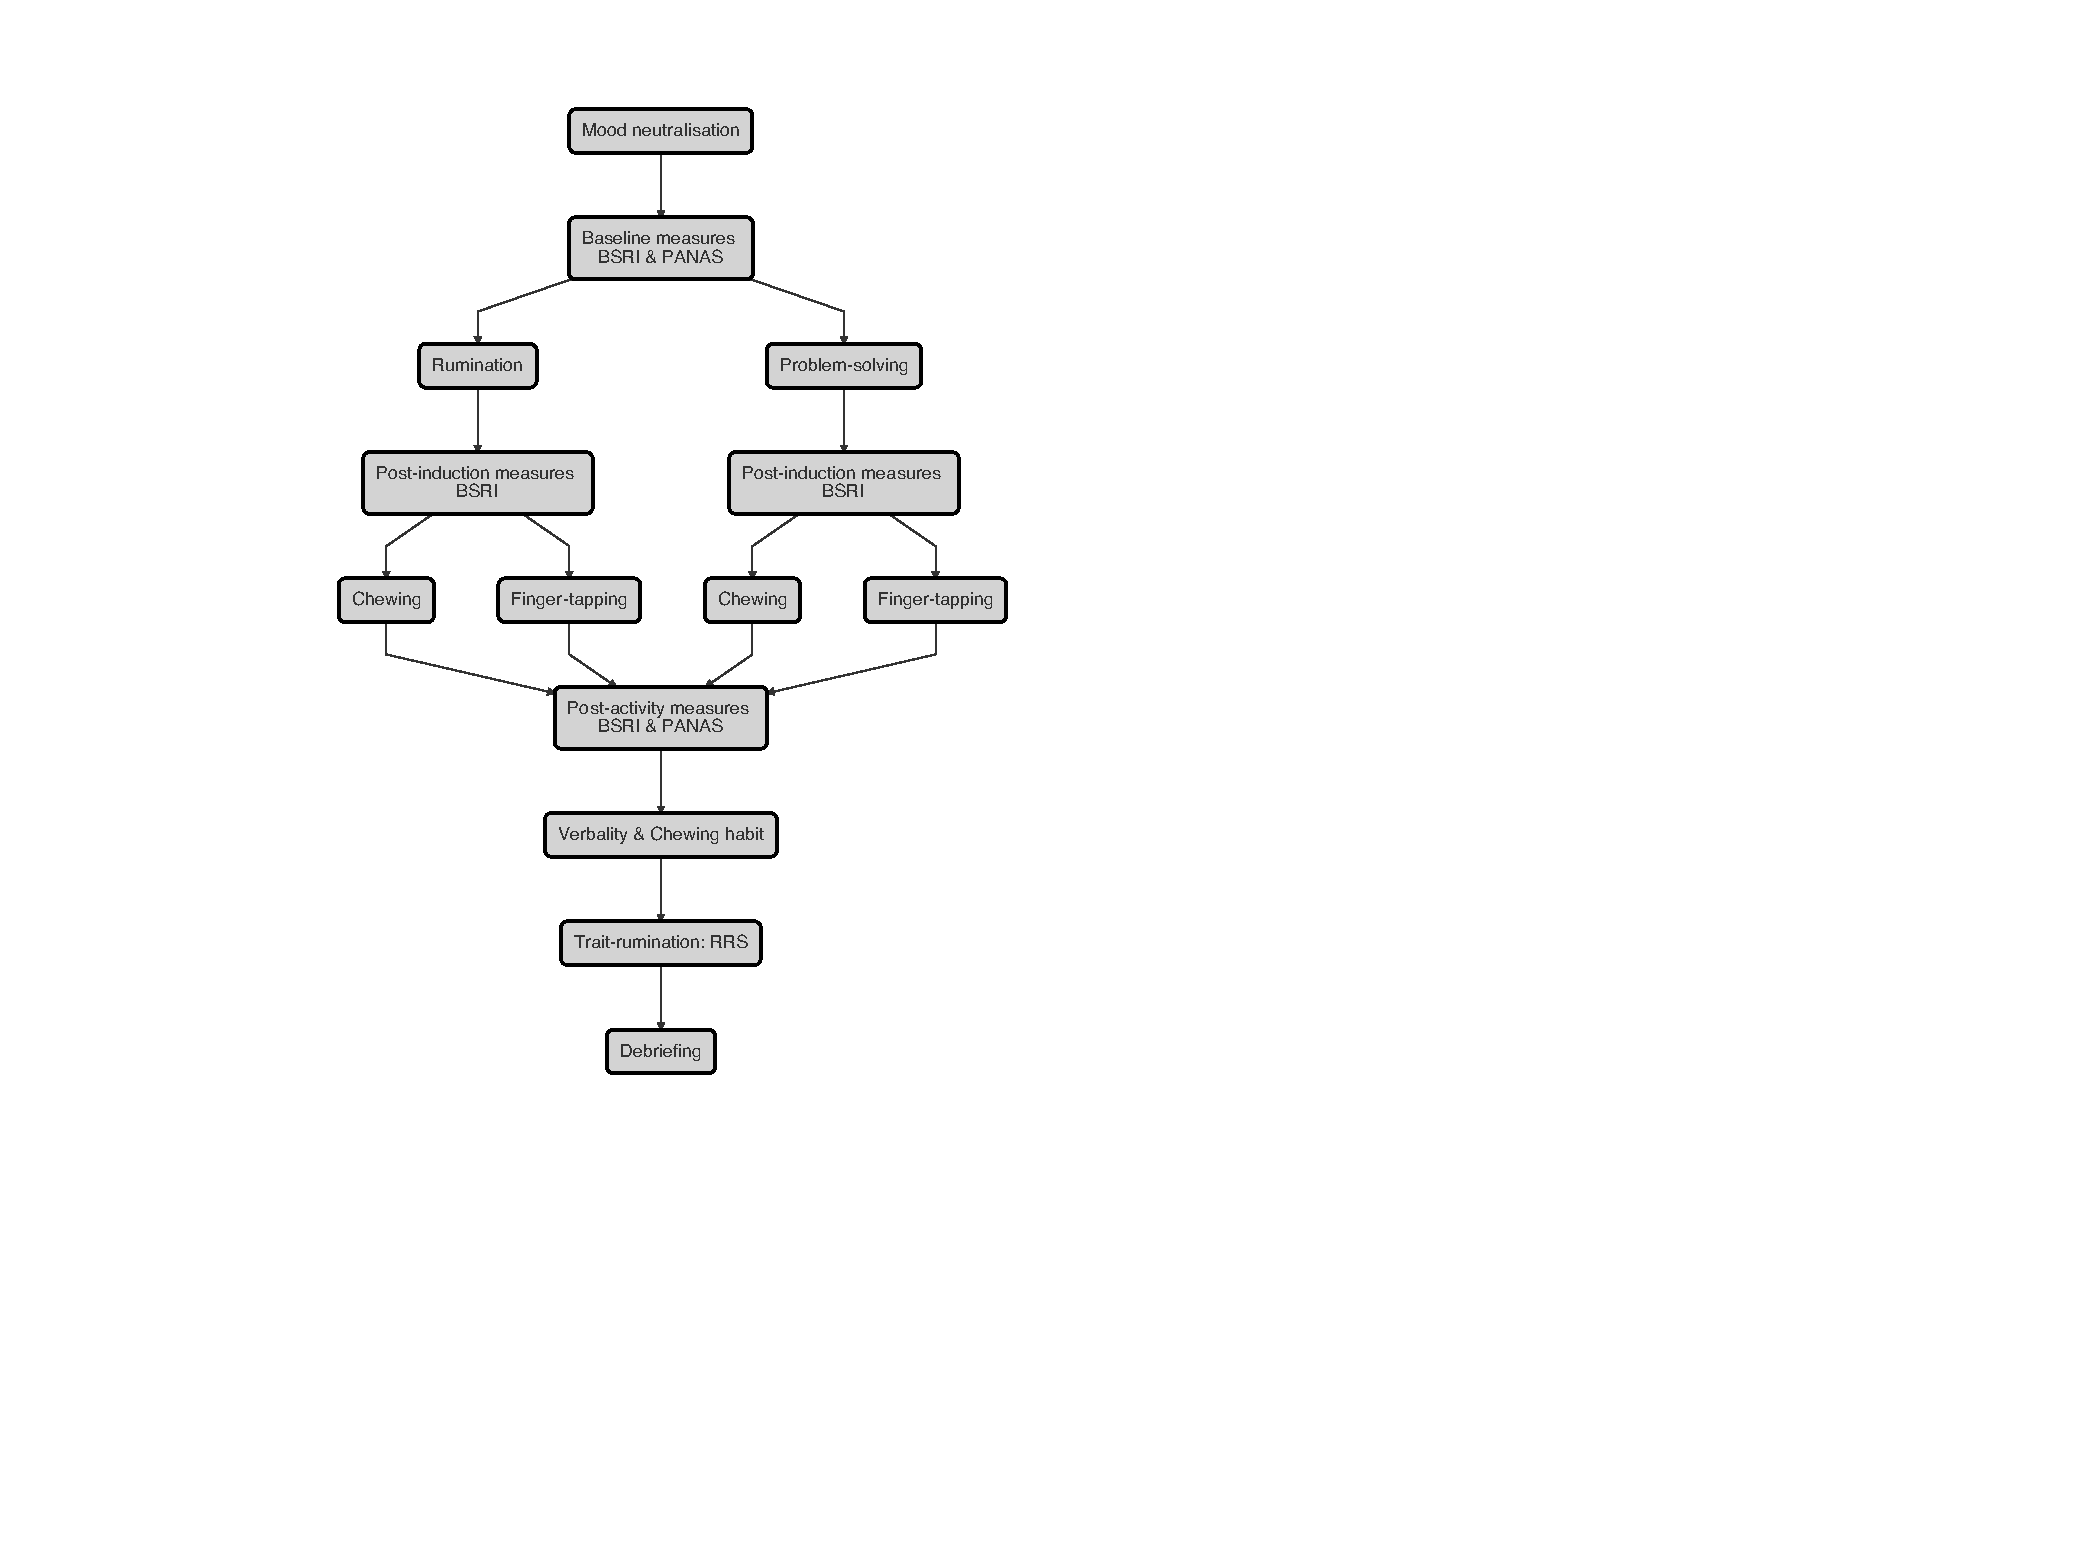
\includegraphics{06-chap6_files/figure-latex/diagram-1} 

}

\caption{Timeline of the experiment, from top to bottom.}\label{fig:diagram}
\end{figure}

\subsection{Data analysis}\label{data-analysis}

Statistical analyses were conducted using R version 3.4.3
\citep{R-base}, and are reported with the \texttt{papaja}
\citep{R-papaja} and \texttt{knitr} \citep{R-knitr} packages.

\subsubsection{Rumination induction}\label{rumination-induction-1}

We centered and standardised each predictor in order to facilitate the
interpretation of parameters. Data were then analysed using
\emph{Induction} (2 modalities, before and after induction,
contrast-coded) as a within-subject categorical predictor and \emph{RUM}
as a dependent variable in a multilevel linear model (MLM). Data were
fitted using the \texttt{lmer} function, within the \texttt{lme4}
package \citep{lme4}. This model was compared with more complex models
including effects of control variables, such as baseline affect state
(\emph{PANAS} scores) or the vividness of the memory chosen during the
induction (\emph{Vividness} score). Models were compared using the
corrected Akaike Information Criterion (AICc) and evidence ratios
\citep{Burnham2002, Burnham2011, Hegyi2011}. AICc provides a relative
measure of predictive accuracy of the models (the AIC is an
approximation of the out-of-sample deviance of a model) and balances
underfitting and overfitting by sanctioning models for their number of
parameters. We computed the difference between the best (lower) and
other AICcs with \(\Delta_{AICc}=AICc_{i}-AICc_{min}\) and then
expressed the weight of a model as:

\[w_{i}=\dfrac{exp(-\Delta_{i}/2)}{\sum_{r=1}^{R}exp(-\Delta_{r}/2)}\]

From there, we computed evidence ratios (ERs) as the ratios of weights:
\(ER_{ij} = \dfrac{w_{i}}{w_{j}}\), where \(w_{i}\) and \(w_{j}\) are
the Akaike weights of models \(i\) and \(j\), respectively. These
weights can be interpreted as the probability of the model being the
best model in terms of out-of-sample prediction \citep{Burnham2002}.
Instead of reporting null-hypothesis tests for our MLMs, we report 95\%
confidence intervals for the constant effects estimates\footnote{These
  may be interpreted as tests of significance: if the confidence
  interval for an estimated parameter does not contain zero, this
  estimate may be considered significant at \(\alpha\) \textless{}.05.}.

Whereas the use of AICc is appropriate for model comparison and
selection, it tells us nothing about the absolute fit of the model. To
estimate this fit, we computed two types of \(R^2\) for MLMs using the
\texttt{MuMIn} package \citep{MuMIn}. The first, called the marginal
\(R^2\) (\(R^2_{marg.}\)), estimates the proportion of variance
accounted for by the constant effects, whereas the second, called the
conditional \(R^2\) (\(R^2_{cond.}\)), estimates the proportion of
variance accounted for by the constant and the varying effects taken
together \citep{Getz2015, Johnson2014, Nakagawa2013}.

\subsubsection{Articulatory suppression
effects}\label{articulatory-suppression-effects}

Data were analysed in the same fashion as in the first part of the
experiment, using \emph{Session} (2 modalities, before and after motor
activity, contrast-coded) as a within-subject categorical predictor, and
\emph{Condition} (2 modalities, Mouthing and Tapping) as a
between-subject categorical predictor and \emph{RUM} as a dependent
variable, in a MLM.

\section{Results}\label{results-1}

\subsection{Correlation matrix between main predictors and control
variables}\label{correlation-matrix-between-main-predictors-and-control-variables}

In order to prevent multicollinearity, we estimated the correlation
between each pair of continuous predictors. Figure \ref{fig:correxp1}
displays these correlations along with the marginal distribution of each
variable. The absence of strong correlations (\(r > 0.8\)) between any
of these variables suggests that they can each be included as control
variables in the following statistical models. Summary statistics (mean
and standard deviation) for all these variables can be found in Table
\ref{tab:sumstat}.

\begin{figure}
\centering
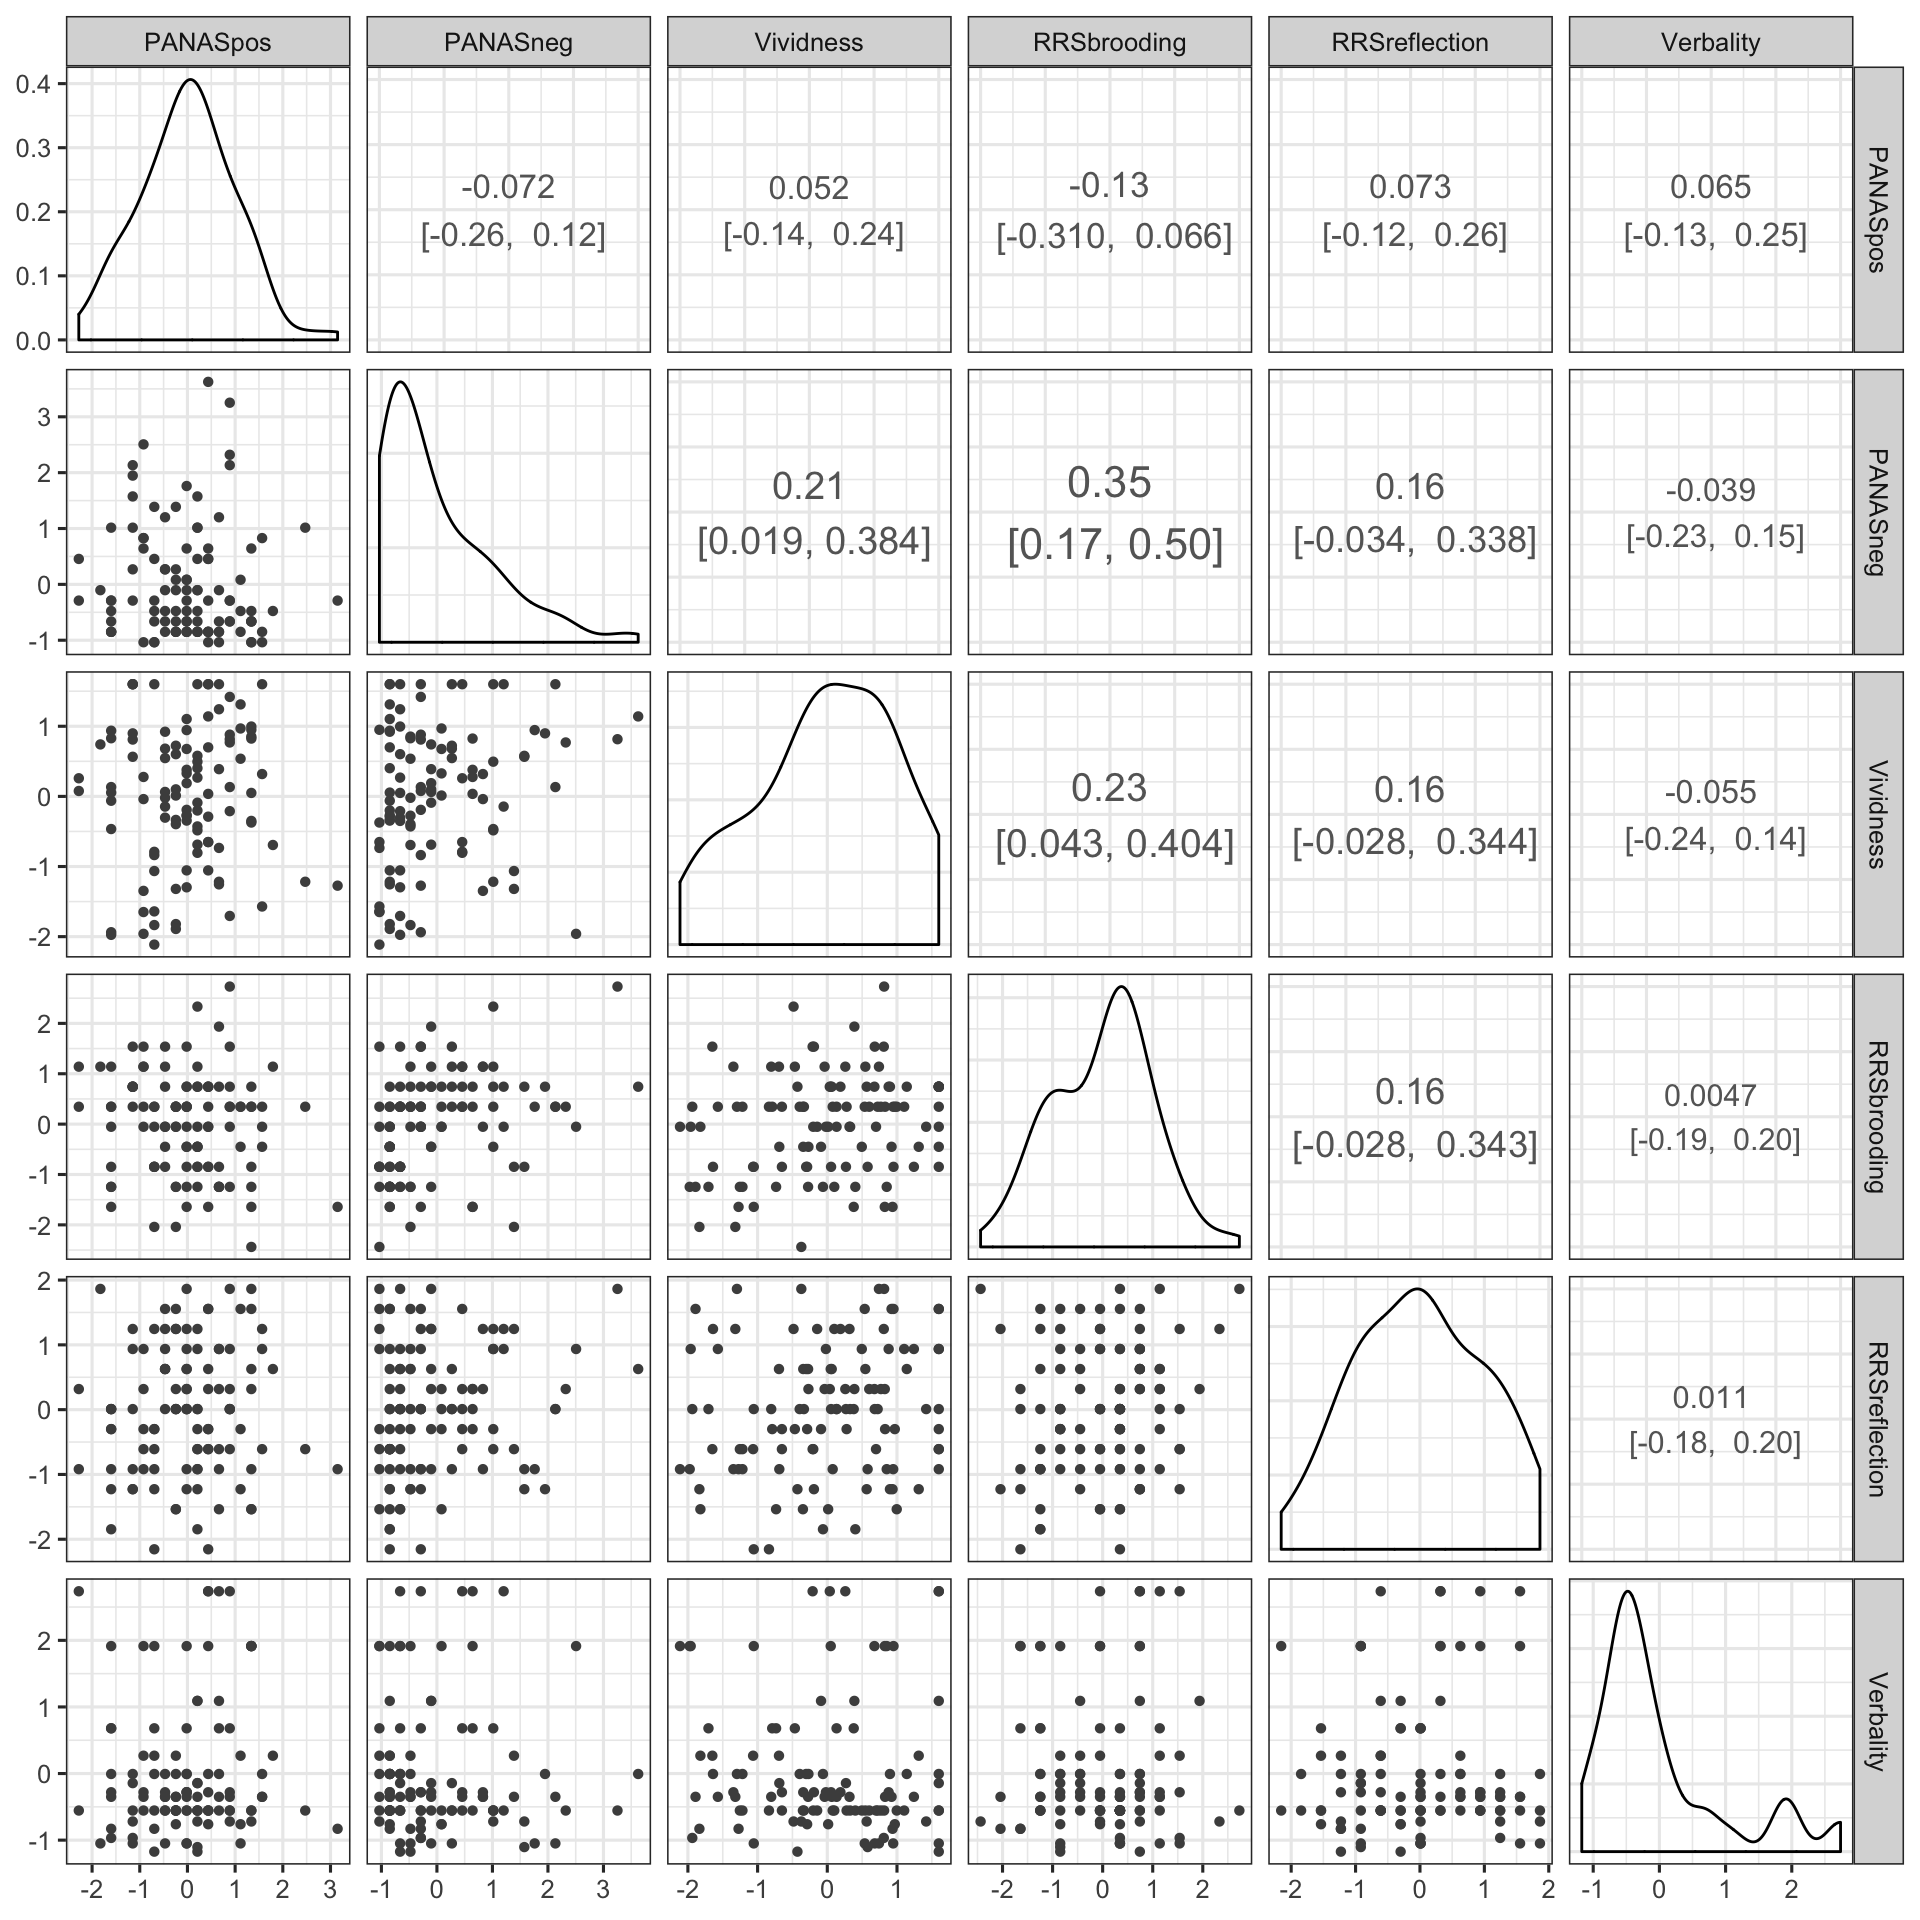
\includegraphics{06-chap6_files/figure-latex/correxp1-1.pdf}
\caption{\label{fig:correxp1}Diagonal: marginal distribution of each
variable. Panels above the diagonal: Pearson's correlations between main
continuous predictors, along with 95\% CIs. The absolute size of the
correlation coefficient is represented by the size of the text (lower
coefficients appear as smaller). Panels below the diagonal: scatterplot
of each variables pair.}
\end{figure}

\begin{table}

\caption{\label{tab:sumstat}Descriptive statistics (mean and standard deviation) of each recorded variable, for the final sample of participants that were included in the study.}
\centering
\begin{tabular}[t]{l|c|c|c|c|c|c}
\hline
Variables & Baseline & Post-induction & Post-motor & Baseline & Post-induction & Post-motor\\
\hline
RUM & 28.5 (26.49) & 54.66 (25.16) & 45.47 (27.25) & 20.96 (21.82) & 46.77 (25.74) & 43.54 (29.57)\\
\hline
Age & 20.3 (2.65) & - & - & 20.31 (2.53) & - & -\\
\hline
PANASneg & 15.65 (5.67) & - & - & 15.46 (5.08) & - & -\\
\hline
PANASpos & 30.91 (4.48) & - & - & 31.25 (4.4) & - & -\\
\hline
RRSbrooding & 12.2 (2.43) & - & - & 12.06 (2.62) & - & -\\
\hline
RRSreflection & 12.22 (3.22) & - & - & 11.71 (3.26) & - & -\\
\hline
Valence & 23.56 (22.4) & - & - & 37.53 (24.61) & - & -\\
\hline
Verbality & 1.67 (1.18) & - & - & 1.67 (1.26) & - & -\\
\hline
Vividness & 54.17 (28.94) & - & - & 59.78 (24.63) & - & -\\
\hline
\end{tabular}
\end{table}

\subsection{Rumination induction}\label{rumination-induction-2}

To examine the efficiency of the induction procedure (i.e., the effect
of \emph{Induction}) while controlling for the other variables (i.e.,
\emph{Vividness}, \emph{RRSbrooding}, \emph{RRSreflection},
\emph{PANASpos}, and \emph{PANASneg}), we then compared the parsimony of
models containing main constant effects and a varying intercept for
\emph{Participant}. Model comparison showed that the best model (in the
sense of the lowest AICc model) was the model including
\emph{Induction}, \emph{PANASpos}, \emph{PANASneg}, \emph{RRSbooding},
and an interaction term between \emph{Induction} and \emph{Vividness} as
predictors (see Table \ref{tab:compexp1}). Fit of the best model was
moderate as marginal \(R^{2}\) was of 0.3801215 while conditional
\(R^{2}\) was of 0.6838429.

\begin{table}

\caption{\label{tab:compexp1}Comparison of models, ordered by AICc relative to the model with the lowest AICc.}
\centering
\begin{tabular}[t]{l|l|c|c|c}
\hline
  & $K$ & $AICc$ & $\Delta_{AICc}$ & $Weight$\\
\hline
$Int+Ind+PANASpos+PANASneg+Ind:Viv+RRSbro$ & 8 & 1903 & 0 & 0\\
\hline
$Int+Ind+PANASpos+PANASneg+Ind:Viv+RRSref$ & 8 & 1903 & 0 & 0\\
\hline
$Int+Ind+PANASpos+PANASneg+Ind:Viv+RRSbro+RRSref$ & 9 & 1904 & 1 & 0\\
\hline
$Int+Ind+PANASneg+Ind:Viv$ & 6 & 1914 & 11 & 0\\
\hline
$Int+Ind+PANASneg$ & 5 & 1916 & 12 & 0\\
\hline
$Int+Ind+PANASpos+Ind:Viv$ & 6 & 1917 & 14 & 0\\
\hline
$Int+Ind+PANASpos$ & 5 & 1919 & 15 & 0\\
\hline
$Int+Ind+Ind:Viv$ & 5 & 1928 & 25 & 0\\
\hline
$Int+Ind$ & 4 & 1930 & 27 & 0\\
\hline
\end{tabular}
\end{table}

Constant effect estimates for the best model are reported in Table
\ref{tab:paramexp1}. Based on these values, it seems that
\emph{Induction} (i.e., the effects of the rumination induction)
increased \emph{RUM} scores by approximately 26 points in average
(\(d_{av} =\) 1.037, 95\% CI {[}0.748, 1.325{]}). The main negative
effect of \emph{PANASneg} and the main positive effects of
\emph{PANASpos} indicate, respectively, that negative baseline mood was
associated with higher levels of rumination while positive baseline mood
was associated with lower levels of self-reported rumination.

\textbackslash{}begin\{table\}

\textbackslash{}caption\{\label{tab:paramexp1}Coefficient estimates (Est),
standard errors (SE), and 95\% CIs (Lower, Upper).\} \centering

\begin{tabular}[t]{l|c|c|c|c}
\hline
 & Est & SE & Lower & Upper\\
\hline
(Intercept) & 37.796 & 1.859 & 34.153 & 41.438\\
\hline
Induction & 25.986 & 2.175 & 21.724 & 30.249\\
\hline
PANASpos & -6.805 & 1.877 & -10.485 & -3.126\\
\hline
PANASneg & 6.995 & 1.986 & 3.104 & 10.887\\
\hline
RRSbrooding & 2.688 & 1.997 & -1.225 & 6.601\\
\hline
Induction:Vividness & 4.273 & 2.178 & 0.003 & 8.542\\
\hline
\end{tabular}

\textbackslash{}end\{table\}

Higher scores on \emph{Vividness} were associated with higher increase
in self-reported rumination after induction, as revealed by the positive
coefficient of the interaction term. This suggests that participants who
recalled a more vivid negative memory tended to show a higher increase
in rumination after the induction procedure than participants with a
less vivid memory.

\section{Articulatory suppression effects on induced
rumination}\label{articulatory-suppression-effects-on-induced-rumination-1}

We then examined the effect of the two motor tasks (articulatory
suppression and finger-tapping) on \emph{RUM}, while controlling for
other variables (i.e., \emph{Vividness}, \emph{RRSbrooding},
\emph{RRSreflection}, \emph{Verbality}, \emph{PANASpos}, and
\emph{PANASneg}). Given the group differences on \emph{RUM} score at
baseline (i.e., after training), we also included this score as a
control variable in our models, as the \emph{RUMb} variable. Based on
our hypotheses, we expected that the model comparison would reveal a
three-way interaction between \emph{Session}, \emph{Condition} and
\emph{Verbality}. However, the best model identified by AICc model
comparison did not include this interaction as a constant effect.
Nonetheless, the best model was only slightly better than the model
including the three-way interaction (the second model in Table
\ref{tab:compexp2}), as the best model was only 1.1704261 more
\emph{credible} than the interaction model. As our goal is precise
estimation of effects rather than dichotomic decision about the presence
or absence of an effect, we chose to present the estimations of the
second model as well. Fit of this model was moderate as marginal
\(R^{2}\) was 0.2928069 while conditional \(R^{2}\) was 0.6626111.

\begin{table}

\caption{\label{tab:compexp2}Comparison of models, ordered by AICc relative to the model with the lowest AICc.}
\centering
\begin{tabular}[t]{l|l|c|c|c}
\hline
  & $K$ & $AICc$ & $\Delta_{AICc}$ & $Weight$\\
\hline
$Int+Session+Cond+RUMb+PANASneg+RRSbro+RRSref$ & 9 & 1914 & 0 & 0\\
\hline
$Int+Session+Cond+Session:Cond+RUMb+PANASneg+RRSbro+RRSref$ & 10 & 1914 & 0 & 0\\
\hline
$Int+Session+Cond+Session:Cond+Session:Cond:Verb+RUMb+PANASneg+RRSbro+RRSref$ & 11 & 1916 & 3 & 0\\
\hline
$Int+Session$ & 4 & 1947 & 33 & 0\\
\hline
$Int+Session+Cond$ & 5 & 1948 & 34 & 0\\
\hline
$Int+Session+Cond+Session:Cond$ & 6 & 1948 & 34 & 0\\
\hline
$Int+Session+Cond+Session:Cond:Verb$ & 7 & 1950 & 36 & 0\\
\hline
$Int$ & 3 & 1953 & 39 & 0\\
\hline
\end{tabular}
\end{table}

Parameter values of the best model for the second part of the experiment
are reported in Table \ref{tab:paramexp2}. Based on these values, it
seems that self-reported rumination decreased after both motor tasks
(the coefficient for \emph{Session} is negative), but this decrease was
substantially larger in the \emph{Mouthing} condition (\(d_{av} =\)
-0.351, 95\% CI {[}-0.735, 0.034{]}) than in the \emph{Tapping}
condition (\(d_{av} =\) -0.117, 95\% CI {[}-0.506, 0.273{]}), as can be
read from the coefficient of the interaction term between \emph{Session}
and \emph{Condition} (\emph{Est} = 5.965, \emph{SE} = 4.320, \emph{95\%
CI} {[}-2.502, 14.433{]}). However, the large uncertainty associated
with this result (as expressed by the width of the confidence interval)
warrants a careful interpretation of this result, that should be
considered as suggestive evidence, rather than conclusive evidence.

The large variation between participants can be appreciated by computing
the \emph{intra-class correlation} (ICC), expressed as
\(\sigma_{intercept}^{2}/(\sigma_{intercept}^{2}+\sigma_{residuals}^{2})\).
For the best model, the ICC is equal to 0.5229, indicating that 52.29\%
of the variance in the outcome that remains after accounting for the
effect of the predictors, is attributable to systematic inter-individual
differences.

\textbackslash{}begin\{table\}

\textbackslash{}caption\{\label{tab:paramexp2}Estimates (Est), standard
errors (SE), and 95\% CIs (Lower, Upper).\} \centering

\begin{tabular}[t]{l|c|c|c|c}
\hline
 & Est & SE & Lower & Upper\\
\hline
(Intercept) & 47.645 & 1.930 & 43.862 & 51.427\\
\hline
Session & -6.214 & 2.160 & -10.448 & -1.980\\
\hline
Condition & -0.948 & 3.921 & -8.633 & 6.736\\
\hline
RUMbaseline & 13.394 & 2.205 & 9.073 & 17.716\\
\hline
RRSbrooding & 2.449 & 2.088 & -1.643 & 6.541\\
\hline
RRSreflection & -2.039 & 1.981 & -5.921 & 1.843\\
\hline
PANASneg & 0.300 & 2.245 & -4.100 & 4.700\\
\hline
Session:Condition & 5.965 & 4.320 & -2.502 & 14.433\\
\hline
sd\_(Intercept).Participant & 16.462 & NA & NA & NA\\
\hline
sd\_Observation.Residual & 15.724 & NA & NA & NA\\
\hline
\end{tabular}

\textbackslash{}end\{table\}

Figure \ref{fig:plotexp1} shows the evolution of the mean \emph{RUM}
scores all through the experiment according to each session (Baseline,
Post-induction, Post-motor) and \emph{Condition} (Mouthing, Tapping).
This figure reveals important inter-individual variability, in all
conditions. After the rumination induction, \emph{RUM} score increased
in both groups, and decreased after the motor task, with a stronger
decrease in the \emph{Mouthing} condition.

\begin{figure}
\centering
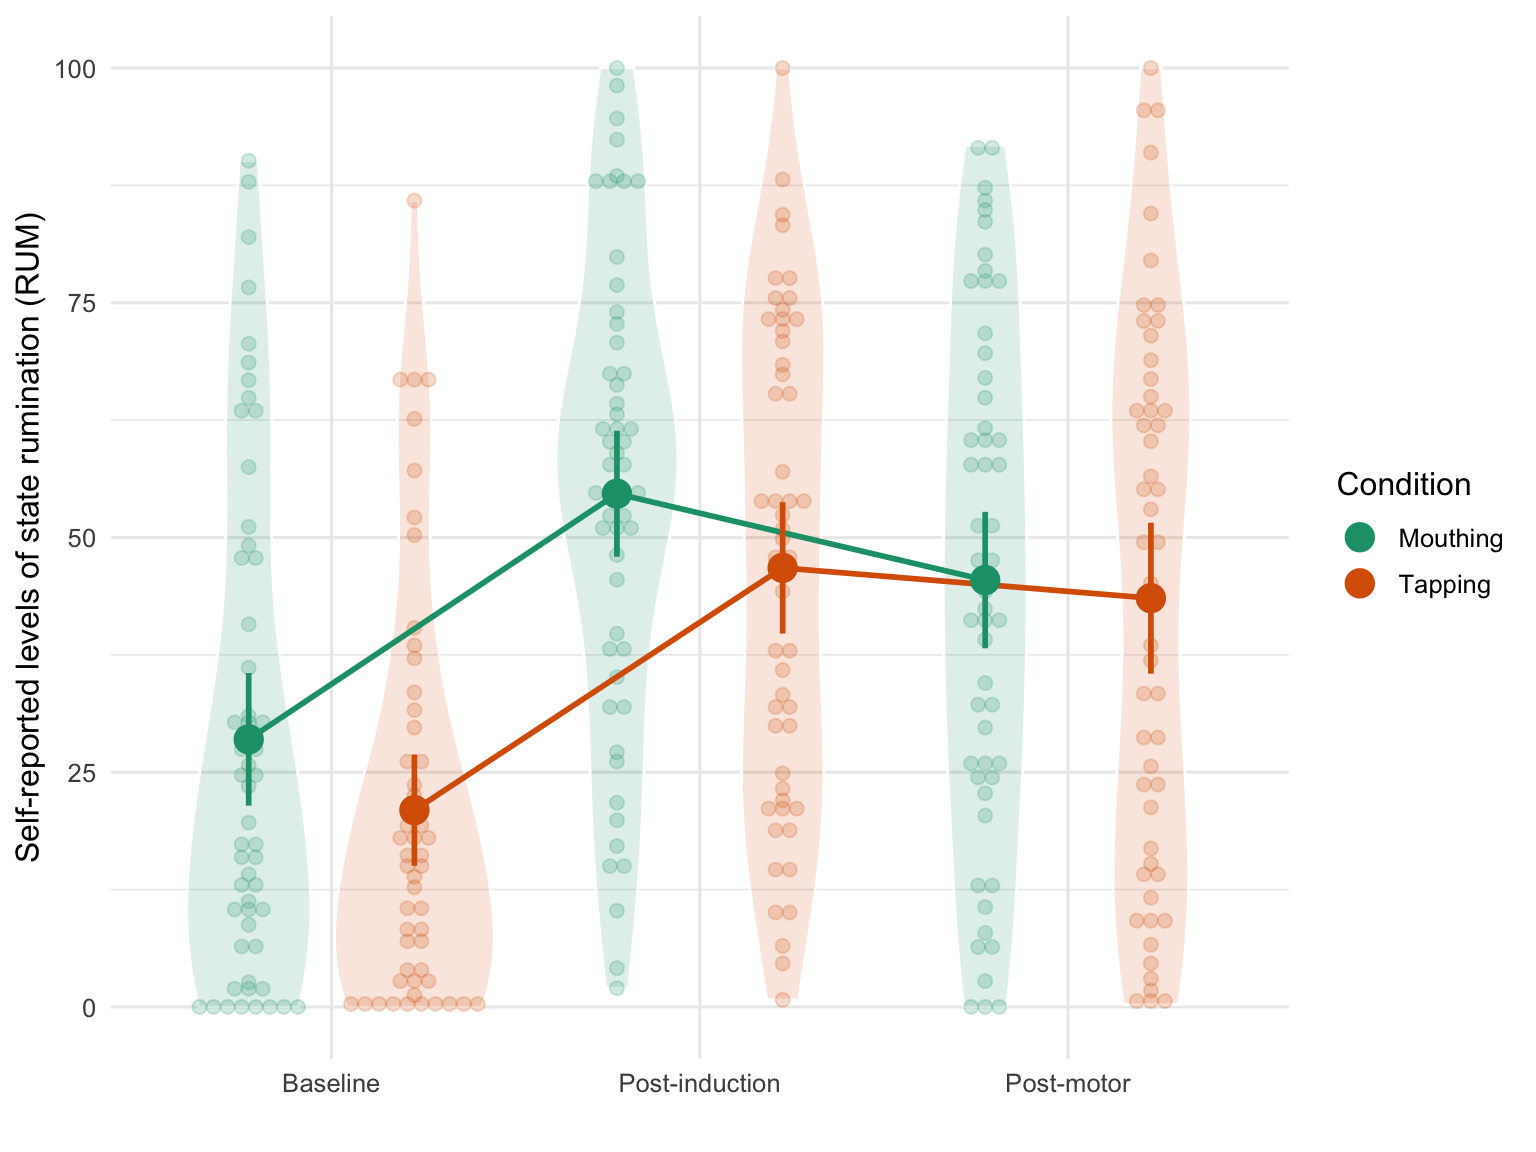
\includegraphics{06-chap6_files/figure-latex/plotexp1-1.pdf}
\caption{\label{fig:plotexp1}Mean RUM score by Session and Condition, along
with violin plots and individual data. Error bars represent 95\% CIs.
The horizontal bar inside the violin plots represents the median of the
conditional distribution.}
\end{figure}

Figure \ref{fig:plotverbal} shows the effects of \emph{Verbality} on the
relative change (i.e., after - before) in self-reported rumination after
both motor activities (i.e., \emph{Mouthing} and \emph{Tapping}). As
\emph{Verbality} was centered before analysis, its score cannot be
interpreted in absolute terms. However, a high score on this index
indicates more verbal than non-verbal (e.g., visual images, non-speech
sounds) thoughts, while a low score indicates more non-verbal than
verbal thoughts. Contrary to our predictions but consistent with the
model comparison, this figure depicts a similar relationship between
\emph{Verbality} and the change in \emph{RUM} score (between before and
after the motor task), according to the Condition.

\begin{figure}
\centering
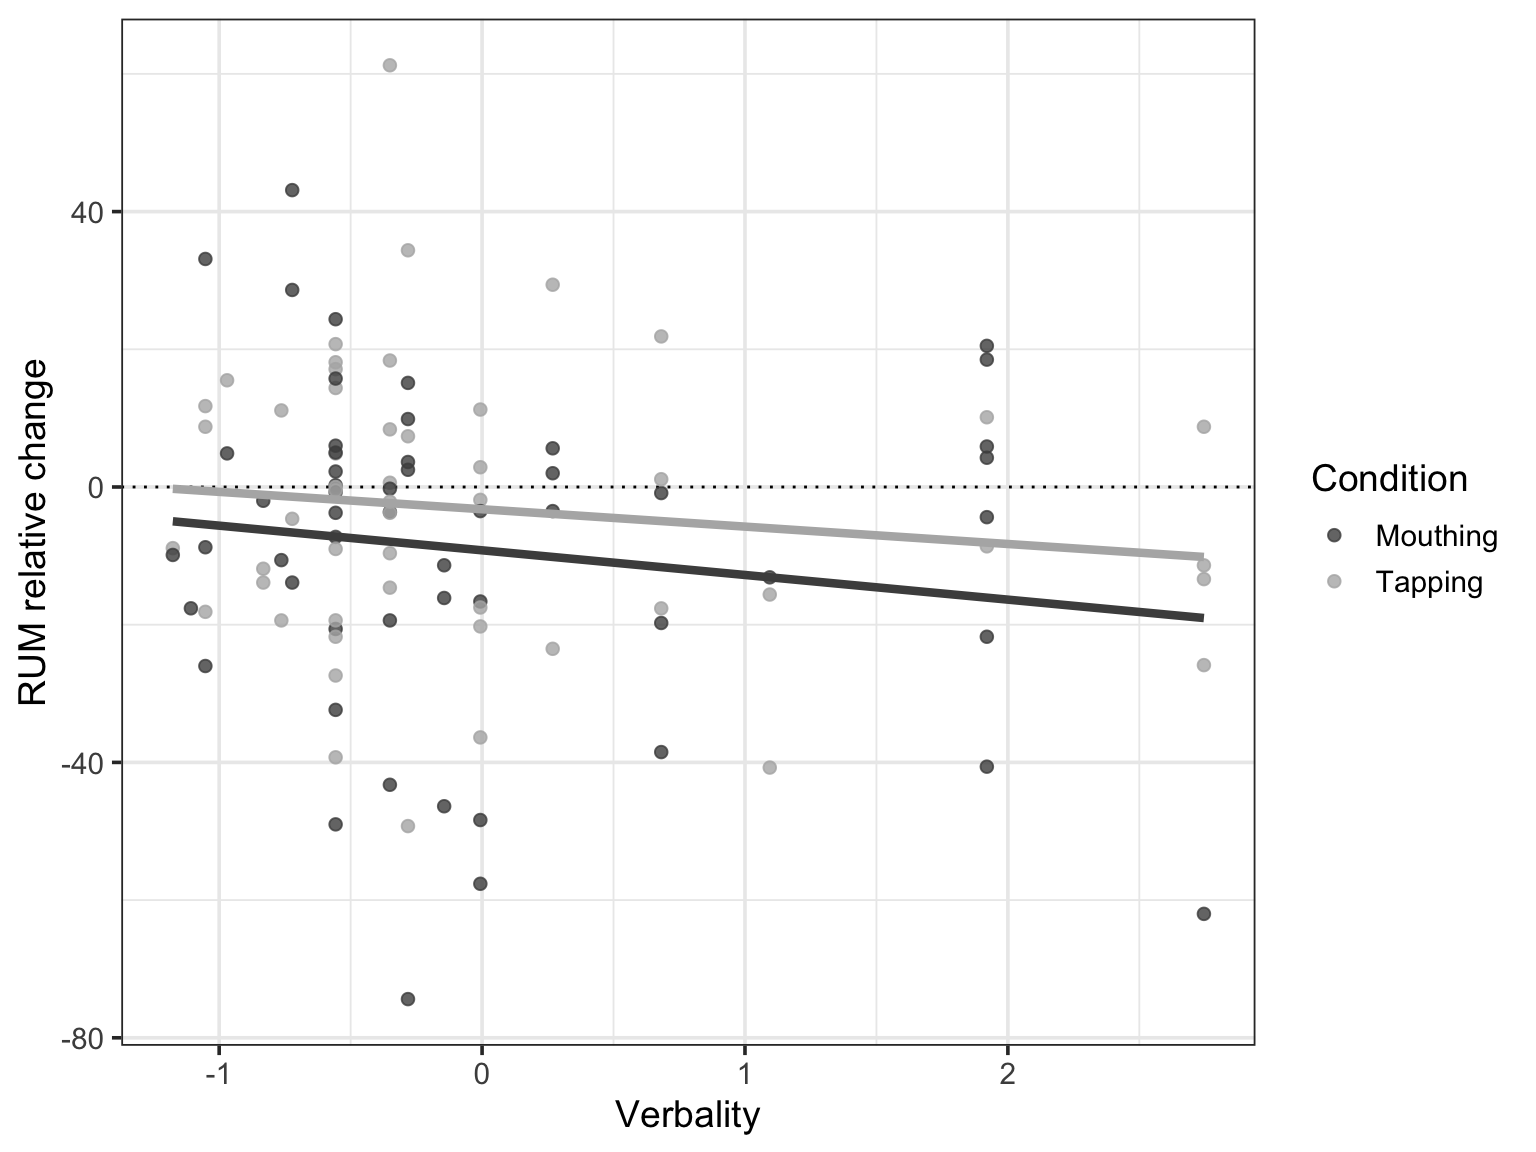
\includegraphics{06-chap6_files/figure-latex/plotverbal-1.pdf}
\caption{\label{fig:plotverbal}Mean RUM relative change after motor
activity, as a function of the degree of Verbality, in the mouthing (the
dark grey dots and regression line) and finger tapping (the light grey
dots and regression line) conditions.}
\end{figure}

\section{Discussion}\label{discussion-1}

The purpose of the current study was to investigate the effects of
articulatory suppression on induced verbal rumination. We predicted that
if verbal rumination, which can be construed as a type of inner speech,
does involve the mental simulation of overt speech production, its
generation should be disrupted by articulatory suppression, but not by
finger tapping. This prediction was not strictly corroborated by the
data, as we observed a decrease of self-reported rumination after both
types of motor activities (see Figure \ref{fig:plotexp1} and Table
\ref{tab:compexp2}), with a somewhat stronger decrease in the Mouthing
condition. In the following, we examine the validity of our methods and
discuss interpretations of our results. Finally, we formulate how
subsequent research should address this kind of question and suggest
alternative ways to test the above mentioned hypothesis. We begin by
discussing the results of the rumination induction procedure.

\subsection{Rumination induction}\label{rumination-induction-3}

It is noteworthy that 32.91\% of the total sample of participants who
were recruited did not respond to this induction, and were therefore not
included in the analyses. Moreover, as reported in Table
\ref{tab:paramexp1}, it seems that the \emph{Vividness} of the memory
chosen by the participant during the mood induction was moderating the
effect of the rumination induction. In other words, the more vivid
(i.e., the more ``intense'') the memory, the more successful the
rumination induction was. This highlights the fact that this aspect
should be carefully controlled each time a mood induction is used in
order to foster subsequent repetitive negative thinking.

Moreover, we observed a group difference of approximately 7.5 points in
the average \emph{RUM} score at baseline. This difference might be
explained by motor training, which took place before baseline
measurement of state rumination. During this training, participants had
to perform the motor task (either finger-tapping or mouthing) in front
of a screen on which a white dot was moving randomly on a black screen,
for 1 min. During the task, the experimenter stayed in the room (out of
the participant's sight) to check that participants were performing the
motor task adequately. Being an unusual and potentially embarrassing
motor activity, mouthing might have been an higher source of stress for
the participants, as compared to the more common activity of
finger-tapping. This group difference in baseline state rumination
subsisted after the induction, as the group difference after the
induction is of approximately 8 points (see full dataset and summary
statistics in the \protect\hyperlink{supp}{supplementary materials}).

\subsection{Articulatory suppression
effects}\label{articulatory-suppression-effects-1}

In the following section, we discuss in more depth the results of the
second part of the study, which aimed at comparing the effects of
articulatory suppression and finger-tapping on self-reported rumination.

First, it is important to examine whether our failure to detect the
predicted interaction could come from a lack of statistical power. We
planned 128 participants in order to reach a power of .80 for a targeted
effect size of \(\eta_{p}^{2}=.06\). As explained above, out of the 184
recruited participants, only 106 could be included in the study. With
106 participants, the a priori power was approximately of .70, which is
much higher than the median power in typical psychological studies.

Second, it is important to acknowledge that despite the absence of the
predicted difference between the two conditions in their influence on
the level of self-reported rumination (i.e., \emph{RUM}), both
activities did lead, on average, to a decrease in self-reported
rumination of approximately 6 points on the VAS (as indicated by the
slope for \emph{Session} in Table \ref{tab:paramexp2}). This decrease
might be interpreted in at least two ways. First, it might be explained
by the simple exposition to the VAS and by compliance effects. When
asked to rate their level of rumination again after five minutes of
motor activity, some participants might be prompted to indicate a lower
level of rumination than before the motor task. But compliance effects
could similarly lead participants to consider the motor task as
irritating, and therefore as prone to rumination increase. Some
participants could therefore also be biased towards indicating a higher
level of rumination after the motor task. Second, it might be considered
that this decrease reflects a genuine decrease in rumination. In the
following, we adopt the latter perspective and discuss explanations for
the weak difference between the two conditions.

\subsubsection{Effect of the rumination quality
(verbality)}\label{effect-of-the-rumination-quality-verbality}

Our prediction was that rumination in verbal form would be more
disrupted by mouthing than rumination in non-verbal form, while both
kinds of rumination would not be disrupted (or similarly disrupted) by
finger-tapping. In other words, we hypothesised a three-way interaction,
between the effect of time (i.e., \emph{Session}), \emph{Condition}, and
\emph{Verbality}. In the following, we discuss the absence of this
interaction. Then, we focus on the weak difference between the two
conditions (omitting \emph{Verbality}), and discuss some explanations
for this weak difference.

First, the absence of the three-way interaction might come from a
difficulty for the participants to have clear introspective access to
the ruminative thoughts they experienced during the experiment. For
instance, we know that introspective description of inner speech differs
considerably, between people trained to regularly report on their
episodes of inner speaking, and people without such training
\citep[e.g.,][]{Hurlburt2013}. Moreover, as the \emph{Verbality}
questionnaire was presented at the end of the experiment, one cannot
exclude that it was partly contaminated by recall, which, when done
verbally, has been shown to artificially increase the subjective
verbality index \citep{Hurlburt2011}.

\subsubsection{Difference between motor
conditions}\label{difference-between-motor-conditions}

Leaving the self-reported quality of rumination aside, we now turn to a
discussion of the weak difference between the two conditions. We think
this result can be explained in at least two non-exclusive ways. First,
we could argue that the decrease observed in both conditions was due to
an unexpected effect of finger-tapping on rumination. Second, we could
argue that the effect of the articulatory suppression was somehow weaker
than expected. In the following, we provide arguments and explanations
for each of these possibilities.

Steady finger-tapping is usually considered as a relevant control
condition for evaluating articulatory suppression, since it specifically
recruits the hand motor system and should not interfere with the oral
motor system, while being comparable in terms of general attentional
demands \citep[e.g.,][]{Gruber2001, Logie1987}. However, using more
complex rhythmic patterns of finger-tapping, \citet{Saito1994} observed
a fade-out of the phonological similarity effect in a verbal memory task
with spoken recall, when subjects were asked to tap with either their
right (dominant) or left hand, while the phonological similarity effect
was conserved in the control condition (no tapping). The author
concluded that a complex rhythmic tapping task can suppress the activity
of the articulatory control process, by \emph{suppressing} the running
of speech motor programs \citep[page 185]{Saito1994}. More specifically,
he suggested that complex, non-automatised, rhythmic finger tapping
could use speech motor programs, which are useful to control speech
prosody, and therefore can deal with rhythmic activity. We further
suggest that a novel complex rhythmic task might require silent
verbalisation and, therefore, might itself be an articulatory
suppression task. In line with these findings, another study showed that
for right-handed subjects, tapping with a finger of the right hand is
more effective at interfering with performance of a verbal memory task
than is tapping with a finger of the left hand \citep{Friedman1988}.
Although Friedman et al.'s findings are difficult to interpret, because
task priority was manipulated and this may have led to conflict
resolution, which might have been dealt with differentially according to
the hand involved, they do suggest that a finger tapping task is not
always the best control for articulatory suppression. This might explain
the decrease of self-reported rumination observed in our own study,
after the finger-tapping, and suggests that we might observe different
results by asking participants to tap with the finger of their
non-dominant hand. We think it is important to note for future studies
that our results, together with those of \citet{Saito1994} and
\citet{Friedman1988}, suggest that finger-tapping could in fact
interfere with inner speech. In other words, finger-tapping, with the
dominant hand, is probably not an appropriate control condition when
studying articulatory suppression.

As suggested previously, an alternative way to explain the absence of
differences between the two motor conditions is to suppose that the
effects of the articulatory suppression were weaker than we expected.
The rhythmic mouthing task might have become too automatised to disrupt
inner speech programming. This idea finds some support in the results of
\citet{Saito1997}, who observed an effect of articulatory suppression on
the phonological similarity effect in a memory task only when the
articulatory suppression was \emph{intermittent} (i.e., ``ah, ah,
ah\ldots{}'') but no effect when participants had to utter a continuous
``ah--''. This can be explained by considering that the intermittent
articulatory suppression would impose a greater load on speech motor
programming than the continuous articulatory suppression \citep[page
569]{Saito1997}. In a similar vein, \citet{Macken1995} found stronger
effects of articulatory suppression when participants were asked to
repeat a sequence of different letters than when they were asked to
repeat a single letter. One way to examine this hypothesis with our own
protocol would be to ask participants to make sequences of various mouth
movements, rather than repeating a single movement.

In a broader perspective, relating to the original research question, we
should mention two additional interpretations of our results. So far, we
considered different ways to explain either how the finger-tapping task
could interfere with rumination or how the articulatory suppression task
might have failed to disrupt rumination. However, if we assume that our
scales (especially the \emph{RUM} outcome response and the
\emph{Verbality} scale) are reliable and that the articulatory
suppression was efficient in its intended purpose, we are forced to
admit that either i) rumination is not a type of inner speech that can
be disrupted by peripheral muscle perturbation (i.e., it could be
described as a more abstract form of inner speech) or that ii) inner
speech, more broadly, does not depend on peripheral speech muscle
activity. Although we think that these questions cannot be answered from
our present results, we acknowledge that these two possibilities are
compatible with our results.

In summary, the current research is one of the first behavioral studies
exploring the association between verbal rumination and the speech motor
system. While the observed data did not strictly corroborate our
original hypotheses, we explored several explanations for the weak
difference between articulatory suppression and the control task, and
related our findings to previous works on the role of inner speech in
verbal working memory. These results have important implications for
future studies on articulatory suppression during inner speech or
working memory tasks. More precisely, they highlight the need for
further investigation of the most appropriate control task when studying
the effects of articulatory suppression.

\hypertarget{supp}{\section{Supplementary materials}\label{supp}}

Pre-registered protocol, preprint, data, as well as reproducible code
and figures are available at: \href{http://osf.io/3bh67}{osf.io/3bh67}.

A lot of useful packages have been used for the writing of this paper,
among which the \texttt{papaja} and \texttt{knitr} packages for writing
and formatting \citep{R-papaja, R-knitr}, the \texttt{ggplot2},
\texttt{ggforce}, \texttt{GGally}, \texttt{DiagrammeR}, and
\texttt{plotly} packages for plotting
\citep{R-ggplot2, R-ggforce, R-GGally, R-DiagrammeR, R-plotly}, the
\texttt{AICcmodavg}, and \texttt{Rmisc} packages for data analysis
\citep{R-AICcmodavg, R-Rmisc}, as well as the \texttt{tidyverse} and
\texttt{broom} packages for code writing and formatting
\citep{R-broom, R-tidyverse}.

\section{Acknowledgements}\label{acknowledgements-1}

This project was funded by the ANR project INNERSPEECH (grant number
ANR-13-BSH2-0003-01). The first author of the manuscript is funded by a
fellowship from Université Grenoble Alpes. We thank David Meary for his
technical support in programming the eye-tracking experiment. We thank
Rafael Laboissiere and Brice Beffara for their advice concerning data
analysis.

\section{Appendix A. Eye-tracking control
experiment}\label{appendix-a.-eye-tracking-control-experiment}

The purpose of this control experiment was to demonstrate that the two
motor tasks used in the main experiment, namely, finger tapping and
articulatory suppression (mouth movements) were equivalent in terms of
task difficulty or general dual-task demand \citep{Emerson2003}.
Participants performed a computer-based visual search task (i.e.,
finding a T among an array of Ls), adapted from the \citet{Treisman1980}
paradigm (see below for details).

\subsection{Sample}\label{sample-1}

Twenty-four participants (Mean age = 19.46, SD = 1.18, Min-Max = 18-21,
21 females, 21 right-handed), drawn from the same population (i.e.,
undergraduate psychology students) as the main experiment took part in
this eye-tracking pretest.

\subsection{Sample size}\label{sample-size}

As we aimed to compare four conditions (i.e., visual search (VS) task
alone, VS + finger tapping, VS + foot tapping and VS + mouth movements),
we recruited 24 participants in order to have at least one participant
per order in our random counter-balanced repeated measures design
(\(n = k!\) where \(n\) is the number of possible orders of conditions
for \(k\) conditions, then \(n =4 != 24\)).

\subsection{Material}\label{material-2}

Experiment took place individually in a dark room. Participants had to
seat in front of a 22 inches, Iyama Vision Master Pro 513-MA203DT CRT
Monitor (resolution: 1024x768 pixels, refresh rate: 85 Hz) with a NVIDIA
GeForce 9800 GTX+ graphic processor. A camera-based eye-tracker
(EyeLink\textregistered~1000 from SR Research) with a sampling rate of
250 Hz and a minimum accuracy of 0.5° was used, in the pupil-corneal
reflection tracking mode. Participants were positioned on a seat so as
to keep distance from the camera to the forehead target between 50 and
60 cm. A five-point calibration was completed before presenting stimuli,
at the beginning of each condition.

\subsection{Procedure}\label{procedure-2}

The target (i.e., the letter ``T'') was present at each trial, either on
the right or on the left of the central vertical axis of the grid. The
grid was an array of 6*6 items. Each stimulus was displayed until the
participant response (maximum duration in case of no response: 5
seconds). Each grid of letters was preceded by a central fixation
circle, that was displayed for 500ms after the participant moved his/her
gaze towards it. In order to give their response (``left'' or
``right''), participants had to gaze towards a large filled gray circle,
situated either on the left or on the right side of the grid. Each
participant went through each condition, in a random order. A first
general training session was proposed, at the beginning of the
experiment, using ten items that were not used subsequently in the four
conditions. Each condition was composed of 90 trials (45 left and 45
right), knowing that the first ten trials of each condition were
considered as training trials and thus not included in analysis. All
participants were filmed in order to ensure that they effectively
performed the motor activity. Our measure of interest was the delay
between the apparition of the grid and the participant's response (the
time at which his/her gaze reached the response circle), below referred
to as ``response time'' (RT).

\subsection{Data preprocessing}\label{data-preprocessing}

Raw data from EyeLink\textregistered~includes gaze on screen spatial
coordinates, pupil diameter and forehead target spatial coordinates,
with its distance from the camera. For this experiment, since only RTs
(in ms) of correct trials are interesting, invalid trials (when no
response has been given) and wrong responses were removed from the
analysis.

\subsection{Data analysis}\label{data-analysis-1}

Data were analysed using \emph{Condition} (4 modalities) as a
within-subject predictor and the natural logarithm of the RT as a
dependent variable in a MLM, including a varying intercept for both
\emph{participant} and \emph{item}. Comparisons of interest were
computed using Helmert contrasts. Estimates and confidence intervals are
reported for each comparison in the log scale.

\subsection{Results}\label{results-2}

Results of the MLM are reported in Table \ref{tab:paramET} and Figure
\ref{fig:eyetrack}. Contrast analysis revealed a slight difference
between the \emph{Control} condition and the mean of the three other
conditions (Est = -0.0099591, 95\% CI = {[}-0.015235, -0.0046832{]}) as
well as a slight difference between the \emph{Foot} condition and the
mean of the \emph{Finger} and the \emph{Mouth} conditions (Est =
0.0050298, 95\% CI = {[}-0.0024395, 0.0124992{]}) while no apparent
differences between the \emph{Mouth} and the \emph{Finger} conditions
(Est = -0.0063662, 95\% CI = {[}-0.0192938, 0.0065614{]}).

\begin{table}

\caption{\label{tab:paramET}Coefficient estimates (Est), standard errors (SE), and 95\% CIs (Lower, Upper) of each contrast.}
\centering
\begin{tabular}[t]{l|c|c|c|c}
\hline
 & $Est$ & $SE$ & $Lower$ & $Upper$\\
\hline
$Control\ vs\ all$ & -0.00996 & 0.00269 & -0.01524 & -0.00468\\
\hline
$Foot\ vs\ Finger + Mouth$ & 0.00503 & 0.00381 & -0.00244 & 0.01250\\
\hline
$Finger\ vs\ Mouth$ & -0.00637 & 0.00660 & -0.01929 & 0.00656\\
\hline
\end{tabular}
\end{table}

\begin{figure}
\centering
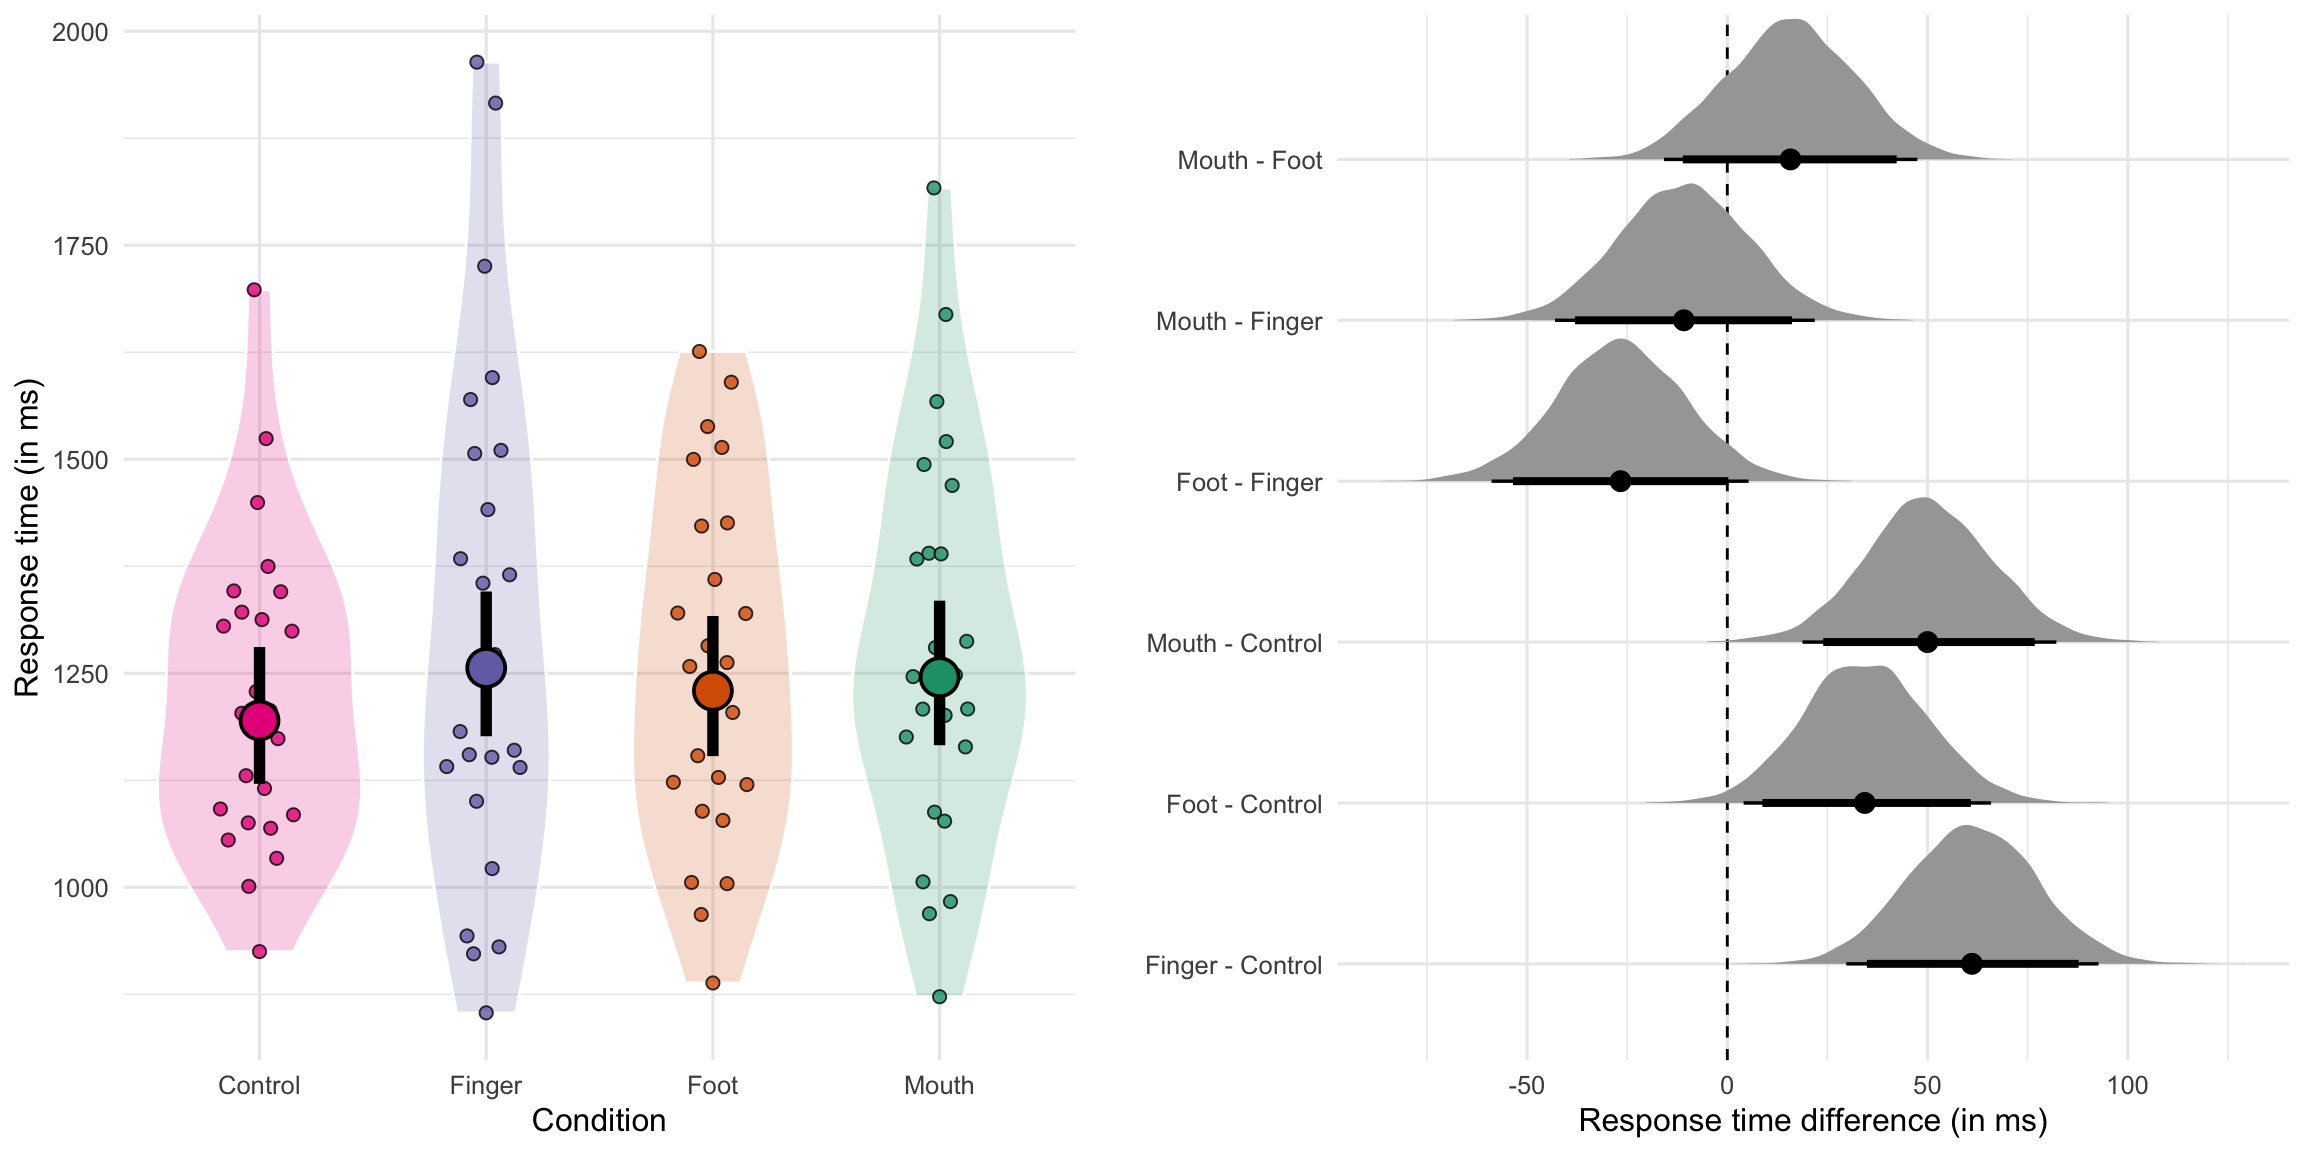
\includegraphics{06-chap6_files/figure-latex/eyetrack-1.pdf}
\caption{\label{fig:eyetrack}Mean RTs by Condition along with 95\% CIs and
violin plots (the horizontal line represents the median of the
conditional distribution). Grey dots represent mean RTs by participant.}
\end{figure}

\subsection{Discussion}\label{discussion-2}

This control experiment shows that there is no apparent difference (or a
negligible one) in terms of attentional demand between the two motor
tasks used in the main experiment (i.e., finger-tapping and mouthing),
although performing a dual motor task (of any type) does seem costly,
because of the observed difference between the control condition and the
mean of the three others conditions. These results are in line with the
results obtained by \citet{Cefidekhanie2014} in their control
experiment.

\chapter{TMS study}\label{tms-study}

\ldots{}

\part{General discussion and
conclusions}\label{part-general-discussion-and-conclusions}

\chapter{General discussion}\label{general-discussion-1}

\ldots{}

\chapter{Conclusions}\label{conclusions}

\ldots{}

\noindent
\setlength{\parindent}{-0.20in} \setlength{\leftskip}{0.20in}
\setlength{\parskip}{8pt}

\bibliography{bib/thesis.bib,bib/packages.bib}


\end{document}
